% main_template.tex - Starter template; copy to notes/<course>/main.tex
% Scaffold for a new course: copy this file, SimpleArticle.sty, and references.bib
% into notes/<course>/, then fill \title / \author below and \include each lecture.

\documentclass[11pt]{article}
\usepackage{SimpleArticle}

\title{FINM 37400: Fixed Income}
\author{Dafu Zhu}
\date{\today}

\begin{document}
\maketitle
\tableofcontents
\newpage

% Uncomment each lecture's \include as its lec0N.tex file is written.
\include{lec01}
\include{lec02}
\include{lec03}
\part*{Lecture 4: Treasury Futures, the Basis Trade, and Swaps}
\addcontentsline{toc}{part}{Lecture 4: Treasury Futures, the Basis Trade, and Swaps}
\beginlecture{04}

Week~4 is the final class session of FINM~37400 (Week~5 is the project and the
closed-book exam; no class meeting). The single 144-minute session covers
three notebooks and revisits a fourth: Treasury futures (\emph{4.2}), with
the cheapest-to-deliver (CTD), conversion factors, gross/net basis, implied
repo, and the embedded options the short holds; swaps (\emph{5.1}), from the
size of the market through the swap-rate formula and the puzzle of negative
swap spreads; a cameo review of floating-rate notes (\emph{2.4}) against
\emph{4.1 Forward Pricing}, which was assigned as reading rather than
lectured on; and a one-sentence preview of the \emph{5.2 Swap-Spread Trade}
case that anchors the next lecture.

\begin{tipblock}
\textbf{Audio dropout.} The lecture recording lost microphone input from
about 28:10 through 85:30 --- roughly 57 minutes that cover the back half of
Treasury Futures (gross/net basis, implied repo, the full CTD computation,
and the embedded options) and the first two cells of Swaps (market size,
definition). The video stream shows the slides the lecturer was on, so the
prose in those sections is reconstructed from frames and the cell text on
the live page, filled in with the standard pedagogy a careful student
would write down. The lecturer's voice returns at~85:30 mid-sentence
(``\emph{\ldots interest rate swap, what is it?}''), and the notes track the
transcript from there.
\end{tipblock}

\section{Forward Pricing (assigned reading)}\label{L4-sec:fwd}

The lecturer skipped \emph{4.1.~Forward Pricing} in the live session (he
opened the class with ``let's jump right back into Treasury Futures'') and
assigned it as prerequisite reading. The page is self-contained and reuses
the FRA algebra from Lecture~2. This section summarizes the parts that the
reader will want on hand for the basis trade below; the full treatment is
on the live page.

\subsection{Forward price as a carry identity}\label{L4-sec:fwd-carry}

\begin{keyblock}
\textbf{Cells~1--9.} \emph{(Page 4.1 \textperiodcentered{} Forward Pricing.)}\\
\textbf{Basics.} A forward agreement is a commitment at $t$ to purchase an
asset at time $T$ for a price $P_{\text{fwd}}$. The rate is set such that
the value of the forward is $0$ when it is entered; the value will change
over time.

\textbf{Synthetic forward.} Replicate the forward by purchasing the asset
at $t$ and financing through term repo to $T$. At $T$, the synthetic long
owns the asset and owes the repo principal plus interest.

\textbf{Carry} in this context is the difference of the coupon of bond $i$
over the financing-rate payment on a dollar-for-dollar repo of the
position. With carry $C$ over $[t,T]$, the forward price satisfies
\[
  P_{\text{fwd}}(t,T)
    \;=\; P(t)\bigl(1 + r_{\text{repo}}\tau\bigr) \;-\; C,
\]
or, rearranged as a \emph{forward drop},
\[
  P_{\text{fwd}}(t,T) - P(t) \;=\; P(t)\,r_{\text{repo}}\tau \;-\; C.
\]
The forward is higher than spot by the financing cost and lower than spot
by the collected coupon.

\textbf{Note.} This relationship is analogous to Covered Interest Parity in
FX, and it will approximately hold in data up to transaction costs and
term-repo illiquidity.
\end{keyblock}

The carry identity is the only piece of \emph{4.1} that the basis trade
below strictly requires. A student who has not read the page should at least
absorb that the forward price of a Treasury is the spot price \emph{grown at
repo} minus the \emph{coupon accrued in the interim}. When the coupon exceeds
the repo cost (``positive carry'') the forward trades at a drop below spot;
when repo exceeds the coupon (``negative carry'') the forward trades at a
rise above spot. This sign convention flips direction a number of times in
the sections below and is worth nailing down before reading on.

\subsection{No-arbitrage price for a coupon bond}\label{L4-sec:fwd-price}

\begin{keyblock}
\textbf{Cells~10--12.} \emph{Forward price with interim coupons.}\\
If the bond pays coupons $c_i$ at times $T_i$ between $t$ and $T$, the
no-arbitrage forward price is
\[
  P_{\text{fwd}}(t,T,T_{\text{bond}})
     \;=\; \frac{P(t) - \sum_{T_i \in (t,T]} c_i \, Z(t,T_i)}{Z(t,T)},
\]
where $P(t)$ is the dirty spot price, $Z(t,T_i)$ is the spot discount
factor to coupon date $T_i$, and $Z(t,T)$ is the spot discount factor to
the forward date $T$. Equivalently, using the forward discount
$F(t,T,T_i) = Z(t,T_i)/Z(t,T)$,
\[
  P_{\text{fwd}}(t,T,T_{\text{bond}})
     \;=\; \frac{P(t)}{Z(t,T)} \;-\; \sum_{T_i\in(t,T]} c_i\,F(t,T,T_i).
\]
\end{keyblock}

The first term in each expression grows the spot price forward at the
financing rate; the second strips out each coupon that will be collected
before the forward matures (those coupons belong to the spot holder, not
to the forward buyer). The page works a specific T-note example (4\%
coupon, 2030-02-28 maturity, 2023 issue) and confirms that Bloomberg's
computed forward price agrees with the identity above.

\subsection{Forwards vs.\ futures and the PV discount}\label{L4-sec:fwd-vs-fut}

\begin{keyblock}
\textbf{Cells~19--38.} \emph{Forwards vs Futures.}\\
Futures differ from forwards in that they
\begin{itemize}
  \item trade on an exchange, not OTC;
  \item trade a standardized contract;
  \item accrue P\&L daily via daily settlement;
  \item require posted margin; and
  \item are intermediated by the exchange (no direct counterparty credit risk).
\end{itemize}
\textbf{Daily settlement reduces bond futures price.} The negative
correlation between rates and the long-futures P\&L is unfavourable to the
long --- when the long wins, rates have fallen and the winnings reinvest at
a lower rate; when the long loses, rates have risen and the losses are
financed at a higher rate. The long therefore bids less for the future
than for the equivalent forward.

\textbf{Tailing the hedge.} Since the futures contract is \emph{more
responsive} to daily movements than a forward (P\&L is realized and
re-investable, not deferred), a hedging desk needs a \emph{smaller} futures
position to match the daily risk of the underlying. The present-value
discount
\[
  N_{\text{fut}} \;=\; N_{\text{fwd}} \cdot Z(t,T)
\]
converts a forward-hedge quantity into a futures-hedge quantity. For
short-horizon contracts ($\tau < 1$ year) one often uses the zero-coupon
discount $Z(t,T)$ directly; for longer horizons, the full convexity
adjustment applies.
\end{keyblock}

The ``rates down / cash received today'' asymmetry is the same mechanism
that produced the STIR-futures convexity adjustment from Lecture~3
\S\ref{L3-sec:stir-tech}: a futures rate is always slightly above the
forward rate on the same underlying, and a futures price is slightly below
the forward price. Tailing the hedge operationalizes this asymmetry for
hedgers, who would otherwise over-hedge if they treated the futures
contract as a zero-cost forward.

\section{Treasury Futures}\label{L4-sec:tf}

With \emph{4.1} in the background, the live class picked up on
\emph{4.2~Treasury Futures} from the beginning. The first 28 minutes
--- before the audio dropout --- covered the volume motivation, the contract
specs, the deliverable basket, and the mechanics of the conversion factor.
The next 57 minutes (through the dropout) walked through gross/net basis,
implied repo, the CTD computation, and the four embedded options held by
the short.

\subsection{Why Treasury Futures --- volume and liquidity}\label{L4-sec:tf-why}

\begin{keyblock}
\textbf{Cells~1--11.} \emph{(Page 4.2 \textperiodcentered{} Treasury Futures.)}\\
\textbf{Why Treasury Futures?} Treasury futures are the most liquid
fixed-income instruments on the exchange. By volume (notional and
DV01-scaled), exchange-listed contracts on the 2-year, 5-year, 10-year,
Long Bond, and Ultra Bond nodes dominate the individual Treasury issues
trading in the cash market.
\begin{center}
\includegraphics[width=0.9\linewidth,height=0.8\textheight,keepaspectratio]{figures/L4_2_c09_volume_zoom.png}\end{center}
Side-by-side bars of notional volume (top) and DV01-scaled volume (bottom)
by instrument; red bars are exchange-listed futures across the duration
grid, blue and green bars are individual Treasury CUSIPs. On the
DV01-scaled measure (bottom panel), the 10-year, Ultra Bond, Long Bond,
5-year, and 2-year futures all beat every individual cash Treasury except
the most recent few on-the-run notes.
\end{keyblock}

The lecturer opened by contrasting the cash and futures markets directly,
reusing the September-markets intuition: futures contracts aggregate
liquidity across a whole maturity bucket into a single exchange-traded
contract, whereas the cash market splits that liquidity across dozens of
CUSIPs --- the four years leading up to a given maturity date each have
several bills, notes, and off-the-run issues, and no single one of them is
especially liquid. A hedger who wants to short a five-year exposure can
either pick one on-the-run five-year note (limited size, narrow bid-ask)
or short one FVM5 future (all the 5-year liquidity on the exchange
collected in one ticker). The second option is almost always easier.

\begin{tipblock}
\textbf{Filling the gap.} The DV01-scaled measure is notional $\times$
modified duration, so it expresses risk transferred per day rather than
face exchanged per day. The reason this matters: a 30-year Long Bond and a
2-year Note at the same notional volume transfer very different amounts of
interest-rate risk. The DV01-scaled chart is the honest comparison for a
trader sizing a hedge --- \emph{how much interest-rate exposure am I
actually shuffling?} --- and it is the measure on which futures beat the
cash market even more decisively than on raw notional.
\end{tipblock}

\subsection{The deliverable basket and conversion factors}\label{L4-sec:tf-basket}

\begin{keyblock}
\textbf{Cells~12--26.} \emph{Delivery, Pricing, and CTD.}\\
In order to increase liquidity, a Treasury futures contract allows
delivery of a range of Treasury notes or bonds, not a single specific
issue. The 10-year futures contract (TY, now TN / Ultra-10) contains
optionality with regard to which Treasury note can be delivered: any U.S.
Treasury note with remaining maturity between $6.5$--$10$ years. The
reason to broaden the basket is to prevent a short from being squeezed
against a single issue that happens to be scarce at delivery.

\textbf{Conversion factors.} The deliverable bonds differ in maturity and
coupon, and the exchange publishes a \emph{conversion factor} $\phi^i$
for each eligible bond $i$. At delivery, the futures settlement price
$\mathcal{F}(T,T)$ is multiplied by $\phi^i$ to determine the cash the
short receives for delivering bond $i$:
\[
  \text{delivery invoice} \;=\; \phi^i\,\mathcal{F}(T,T) + A^i_T,
\]
where $A^i_T$ is accrued interest on bond $i$.

\textbf{Example: FVM5 (5-year T-Note, June 2025 delivery).} On
2025-02-25 the data file lists the seven eligible notes; each has a
conversion factor in the 0.90--0.94 range, reflecting that most of the
deliverable 5-year notes carry a 3.5--4.4\% coupon against the 6\%
published assumption.
\end{keyblock}

The lecturer walked the class through this carefully, because the
conversion-factor idea is deeply non-obvious. Think of the contract as a
long-short auction: the exchange wants a short to be indifferent (at
settlement) between delivering any two bonds in the basket, so that the
short's optionality does not translate into a settlement lottery. The
conversion factor is the exchange's attempt to make that indifference hold
when the basket is evaluated at a single reference rate.

The factor for bond $i$ is computed by pricing bond $i$ at a flat 6\% yield
and dividing by its face,
\[
  \phi^i \;=\; \frac{1}{100}\sum_{j=1}^n \frac{c_i/2}{(1+.06/2)^{2T_{ij}}}
                \;+\; \frac{1}{(1+.06/2)^{2T_{in}}},
\]
where the sum runs over the coupon dates of bond $i$ remaining at the
delivery date. The lecturer walked through why each ingredient is chosen
the way it is.

\emph{Why a single flat rate, and why 6\%?} A single reference rate is the
only way to get a published, immutable conversion factor: the exchange
needs a $\phi^i$ it can print at contract issue and never revise. Using
``today's'' rate (a spot curve or YTM) would make $\phi^i$ move with the
market and defeat the whole purpose of a conversion factor. The specific
value 6\% is the rate the CME used historically when rates were higher;
they left it in place through the low-rate era because it is
\emph{immutable} for each outstanding contract. When the exchange rolls a
new generation of contracts it can change the convention, but the existing
tickers run to expiry on the old rule. The lecturer answered a student
question about whether 6\% was meaningful with ``I mean, I have no idea,
and it really doesn't matter. They just put in any number there.''

\emph{Does the 6\% miscalibration matter?} Because the actual spot curve
is much lower than 6\% (``closer to 4\%'' in 2025), the convention
uniformly \emph{undervalues} every bond in the basket. The lecturer
pressed the class on whether that mattered, and walked them to the
answer: no, because the short picks the cheapest-to-deliver bond and the
relative ranking of bonds is what drives the short's decision. A uniform
undervaluation shifts every delivery price by approximately the same
amount and leaves the CTD ranking unchanged. It also means that $\phi^i$
for a bond whose coupon is below 6\% sits below 1 (demerit); above 6\%
sits above 1 (credit); at 6\% sits exactly at 1. The \$100 face receives
the credit or demerit as a multiplicative scaling --- ``so in some ways you
could say they could look at maybe the yield to maturity. Don't we already
have a metric for that?'' The lecturer's answer to his own question was
that YTM depends on \emph{price}, which is real-time, so using YTM would
make the conversion factor move every second. Present value at a flat 6\%
is the cleanest rule that uses only coupon and maturity.

\begin{tipblock}
\textbf{Filling the gap.} The factor-1 bond is by construction the bond
whose cashflows, when present-valued at 6\%, equal face. For a freshly
issued Treasury this requires coupon $\approx$~6\% and maturity matched to
the contract window. The exchange does not need any such bond to exist in
the basket --- $\phi^i$ is well-defined for each actual deliverable --- but
this observation is useful for sanity-checking the numbers: if two bonds
in the basket have nearly equal coupon and maturity, their $\phi^i$ must
be nearly equal, and the CTD choice between them will be driven by the
cash-market price differential alone.
\end{tipblock}

\subsection{Delivery cost, gross basis, and net basis}\label{L4-sec:tf-basis}

\emph{(Audio gap begins here. The lecturer was working through cells~27--46
of 4.2, ``Gross and Net Basis,'' for the next 45 minutes. The prose below
reconstructs the teaching order from the frames and the cell content; the
formulas are exactly as stated on the live page.)}

\begin{keyblock}
\textbf{Cells~27--35.} \emph{Gross and Net Basis.}\\
\textbf{The basis trade.} Being long the bond's basis means taking a
position of:
\begin{itemize}
  \item long a \emph{forward} bond at the delivery date $T$, financed spot
        via term repo;
  \item short the corresponding futures contract, adjusted by the
        conversion factor.
\end{itemize}

\textbf{Gross basis} measures the basis trade where the bond is transacted
\emph{spot} (no forward), and the futures leg is unadjusted for carry:
\[
  B^i_{t,t+\tau} \;=\; P^i_t \;-\; \phi^i\,\mathcal{F}(t,T).
\]

\textbf{Net basis} measures the same trade but with the spot leg replaced
by a \emph{forward} bond, so it absorbs the carry:
\[
  \tilde B^i_{t,t+\tau} \;=\; P_{\text{fwd}}^i(t,T) \;-\; \phi^i\,\mathcal{F}(t,T).
\]

\textbf{Alternate view.} Since the forward drop equals the bond's carry,
$\tilde B$ can be read as $B^i - \text{carry}$: net basis is gross basis
minus the carry over the contract horizon.
\end{keyblock}

The conceptual shape of the basis trade follows directly from the forward
identity of~\S\ref{L4-sec:fwd-carry}. If the forward price were the only
no-arbitrage price for a Treasury on the delivery date, then after the
conversion-factor adjustment the futures price $\mathcal{F}(t,T)$ would
equal $P_{\text{fwd}}^i(t,T)/\phi^i$ for the CTD bond, and the net basis
for the CTD would be identically zero. The basis trade is the wager that
this equality is \emph{nearly but not exactly} right, and that the
relative ordering of basis values across the deliverable basket tells you
which bond the short will elect to deliver.

The split between gross and net basis matters because Wall Street quotes
the trade in net basis even though it transacts the spot leg: the
quoted number is already carry-adjusted, so a zero gross basis does not
mean a zero-P\&L trade. A trader who pays the gross basis to go long
collects the carry until delivery, and the carry is the \emph{majority}
of the P\&L on most basis trades. The lecturer emphasized this enough on
the live page that the \emph{Alternate View} callout exists precisely to
head off the confusion.

\begin{keyblock}
\textbf{Cells~36--41.} \emph{Examples: Gross and Net Basis (FVM5, 2025-02-25).}\\
\begin{center}
\includegraphics[width=0.9\linewidth,height=0.8\textheight,keepaspectratio]{figures/L4_2_c41_net_basis.png}\end{center}
Bond-by-bond table of coupon, repo rate, days to forward, accrued interest,
dirty price, carry, gross basis, and net basis across the deliverable
basket. All seven bonds share a common $r_{\text{repo}} = 4.37\%$ and a
$124$-day forward interval. Net basis ranges from $+0.07$ (for the
91282CLK 2029-08-31 note) to $+0.56$ (for the 91282CMG 2030-01-31 note) ---
all positive, with the smallest belonging to the CTD.
\end{keyblock}

The student is meant to spot two things in this table. First, net basis is
positive for every bond in the basket: the short's option to select among
bonds extracts a non-zero premium from the long, so the basis trader
\emph{pays} rather than collects this value. Second, the CTD (here 91282CLK)
has the smallest net basis --- not zero, because of the embedded optionality
of~\S\ref{L4-sec:tf-options}, but the smallest among the deliverables. Any
long-CTD / short-future trade earns the carry over the contract horizon and
loses the option premium the short keeps.

\begin{keyblock}
\textbf{Cells~42--46.} \emph{Convergence and caveats.}\\
\textbf{Convergence.} At expiration $T$, gross basis and net basis are
equal ($B^i_T = \tilde B^i_T$, because carry over zero time is zero) and
for the CTD both are zero:
\[
  B_T^{\text{CTD}} \;=\; \tilde B_T^{\text{CTD}} \;=\; 0.
\]

\textbf{Importance of Net Basis.} Net basis is the most commonly quoted
measure because it strips out the predictable carry component and isolates
the trader's bet on the optionality.

\textbf{Daily settlement.} The P\&L of the basis trade as above is only
approximate: daily settlement on the short-futures leg produces
intermediate cashflows that the forward-bond leg does not mirror,
contributing a (usually small) timing wedge.

\textbf{Repo caveat.} The synthetic forward relies on \emph{term} repo
over the contract horizon. In practice, term repo for $\tau$ months may
not be deep enough to fund the position; the trader may have to roll
overnight repo, accepting daily re-pricing of the financing rate.
\end{keyblock}

The two caveats are worth pausing on because they explain why basis
trading is its own desk. Daily settlement means the short leg receives or
pays cash every day, which must be invested or borrowed; the forward leg
has no such cashflow. In a rising-rate environment, the short leg receives
cash on down days and reinvests at the higher new rate, giving the short
a small positive bias; the basis trader has to mark this correction
against the quoted basis when comparing actual to theoretical P\&L. The
repo caveat reminds the trader that the forward-leg construction is an
approximation: term repo is often thin beyond a few weeks, so the
synthetic forward may be reconstructed nightly from overnight repo, with
each roll marked at the prevailing overnight rate. If the repo rate
spikes (as in the September 2019 repo crisis, referenced in
\S\ref{L4-sec:swap-spread-pointer}), the basis trade can be swamped by
financing costs.

\subsection{Implied repo}\label{L4-sec:tf-impliedrepo}

\begin{keyblock}
\textbf{Cells~47--55.} \emph{Implied Repo.}\\
The \textbf{implied repo rate} for bond $i$ is the repo rate that
rationalizes the ``futures-as-forward'' relationship:
\[
   F(t,T)^i \;=\; \mathcal{F}(t,T)\,\phi^i.
\]
Solve for $r^i_{\text{IR}}$ from
\[
   \underbrace{F(t,T)^i + A^i_T}_{\text{dirty forward}}
     \;=\; \underbrace{\bigl[P^i_t + A^i_t\bigr]}_{\text{dirty spot}}
        \bigl[1 + r^i_{\text{IR}}\,\tau_{\text{act}/360}\bigr],
\]
where $r^i_{\text{IR}}$ is the implied repo rate on bond $i$ and
$\tau_{\text{act}/360}$ is the forward interval in years under the
ACT/360 money-market convention.

\textbf{Trading-strategy interpretation.} $r^i_{\text{IR}}$ is the
annualized return from a trader who at time $t$:
\begin{itemize}
  \item buys bond $i$ spot;
  \item shorts the futures contract (with conversion factor $\phi^i$);
  \item holds both to delivery and delivers bond $i$ into the short.
\end{itemize}
If bond $i$ does end up being CTD, $r^i_{\text{IR}}$ is the trader's
realized return. If bond $i$ is \emph{not} CTD, the trader finds that
the price of the (now suboptimal) long-delivery is compromised relative
to the CTD, and the realized return is less than $r^i_{\text{IR}}$.

\textbf{Careful: this implied repo is assuming the bond becomes CTD!} A
high implied repo rate may simply mean the bond is unlikely to become
CTD (so the calculation is based on a counterfactual) rather than a
genuine arbitrage opportunity.
\end{keyblock}

The interpretation the lecturer drives home on this page is the third
bullet: $r^i_{\text{IR}}$ is not a universal ``repo rate implied by the
futures chain'' but a \emph{bond-by-bond} quantity that tells the trader
how much they would earn if they locked in bond $i$'s futures-to-spot
spread through delivery. The trader cannot actually earn $r^i_{\text{IR}}$
on any bond of their choice, because the short-futures leg pays off at
$\phi^{\text{CTD}}\mathcal{F}(T,T)$ regardless of which bond the trader
holds.

\begin{tipblock}
\textbf{Filling the gap.} There is a clean relationship between implied
repo and the CTD rule:
\[
   i^\star \;=\; \arg\max_i r^i_{\text{IR}}.
\]
The bond with the highest implied repo is (by definition) the bond
delivering the highest annualized return through the synthetic-forward
calculation, which is exactly the bond the short would choose to deliver.
A table of implied repo rates ranked across the basket is therefore a
direct CTD screen: the highest number is the short's best choice. The
convenience of ranking by a single annualized number is why desks quote
implied repo alongside net basis --- they carry the same information in
different units, but implied repo is dimensionless (a rate) where net
basis is in dollars.
\end{tipblock}

\subsection{The cheapest-to-deliver computation}\label{L4-sec:tf-ctd}

\begin{keyblock}
\textbf{Cells~56--65.} \emph{Cheapest to Deliver.}\\
\textbf{Conversion factor.} $\phi^i$ is the publicly published, immutable
scaling of the delivery price of bond $i$ at the reference rate of 6\%.

\textbf{Delivery cost.} For a short position, the cost to deliver bond
$i$ to close out the futures contract is
\[
   \text{delivery cost}_T \;=\; \bigl(P^i_T + A^i_T\bigr)
                               \;-\; \bigl(\phi^i\,\mathcal{F}(T,T) + A^i_T\bigr)
                           \;=\; P^i_T \;-\; \phi^i\,\mathcal{F}(T,T).
\]
Accrued interest cancels, so the delivery cost is simply the bond's price
(clean or dirty, they differ by the same $A^i_T$ that cancels) minus the
converted futures price.

\textbf{CTD rule.} Shorts choose to deliver the bond that minimizes
delivery cost:
\begin{align*}
   \text{CTD} &\;=\; \arg\min_i \bigl[P^i_T - \phi^i\,\mathcal{F}(T,T)\bigr] \\
              &\;=\; \arg\min_i \frac{P^i_T}{\phi^i},
\end{align*}
where the second equality holds because $\mathcal{F}(T,T)$ is the same
across all bonds in the basket --- it factors out.

\textbf{Convergence at expiry.} By no-arbitrage, at expiry,
\[
   \mathcal{F}(T,T) \;=\; \frac{P^{\text{CTD}}_T}{\phi^{\text{CTD}}}
                       \;\le\; \frac{P^i_T}{\phi^i} \quad \forall i.
\]

\textbf{Example: CTD Determination.} Bloomberg identifies the CTD Treasury
note along with its gross and net basis.
\begin{center}
\includegraphics[width=0.7\linewidth,height=0.25\textheight,keepaspectratio]{figures/L4_2_c62_bbg_ctd.png}\end{center}
The contract (FVM5 Comdty) shows CTD price $97.93$, gross basis $-5.95$,
and net basis $+1.54$.

\textbf{Confirm the CTD.} Computing $P^i_T - \phi^i\,\mathcal{F}(T,T)$
directly from the bond data for all seven deliverables produces a
delivery-cost column whose minimum flags the CTD.
\begin{center}
\includegraphics[width=0.9\linewidth,height=0.6\textheight,keepaspectratio]{figures/L4_2_c65_confirm_ctd.png}\end{center}
The $91282\mathrm{CLK}$ note (2029-08-31, 3.62\% coupon, $\phi = 0.9135$)
has delivery cost $107.20$, the smallest in the basket --- highlighted in
green as the CTD. The worst candidate, 91282CMG (2030-01-31, 4.25\%), has
delivery cost $107.95$ --- only 75 cents worse, but on a standardized
futures contract that 75 cents is the short's option value.
\end{keyblock}

The \emph{convergence at expiry} identity is the single most important
equation on this page. Before expiry, $\mathcal{F}(t,T)$ is set by the
market; at expiry, the futures price must converge to the price/phi ratio
of whichever bond the short chooses --- and the short chooses to minimize
that ratio. The intuition is the arbitrage argument: if at expiry the
futures price exceeded any bond's $P^i_T/\phi^i$, the short could buy bond
$i$ in the cash market, deliver it into the short-future, and collect the
difference risk-free; the short's demand drives $\mathcal{F}(T,T)$ up to
the cheapest ratio.

The \emph{minimization in delivery cost = minimization in price/phi ratio}
equivalence is why Bloomberg's quoted ``CTD'' column is computed by
ranking the delivery-cost column, not by computing the price/phi ratio
directly: the two rankings agree by construction, and the delivery-cost
column is what traders actually compute at expiry.

\begin{keyblock}
\textbf{Cell~66.} \emph{Technical Point: Calculation of the conversion factor.}\\
Suppose bond $i$ has coupon rate $c_i$ and $n$ coupon periods remaining at
delivery. Its conversion factor is
\[
   \phi^i \;=\; \frac{c_i}{.06}\Bigl(1 - \frac{1}{(1+.06/2)^{2T_{in}}}\Bigr)
              \;+\; \frac{1}{(1+.06/2)^{2T_{in}}}.
\]
(This is the standard present-value formula for an annuity of $c_i/2$
coupon payments plus a 1-of-face principal repayment, discounted at 6\%
semiannual compounding.) Note that $\phi^i$ is constant over the length of
the futures contract; there is no time subscript. The formula depends
only on bond $i$'s coupon rate and its remaining maturity at the contract
delivery date.
\end{keyblock}

\begin{keyblock}
\textbf{Cell~67.} \emph{Understanding CTD.}\\
\textbf{In a low-rate environment} (such as 2008--2021): \emph{lower-coupon,
shorter-maturity} bonds tend to be CTD, because $\phi^i$ shrinks below 1
by less for these bonds under the 6\% convention, and their cash prices
are relatively higher than the 6\%-convention valuations would predict.

\textbf{In a high-rate environment}: \emph{higher-coupon, longer-maturity}
bonds tend to be CTD --- the same mechanism running in reverse.
\end{keyblock}

The CTD story is sensitive to the \emph{difference} between the actual rate
and the 6\% convention. When actual rates are well below 6\% (the norm
2008--2021), the convention undervalues every bond; the degree of
undervaluation is larger for longer maturities (the discount factor
mismatch accumulates), so the conversion factor shrinks more for long
bonds than the market price does, which makes long bonds \emph{more}
expensive to deliver per unit of conversion. The rule of thumb is that
when rates are low, the CTD rotates to the short end of the basket; when
rates are high, it rotates to the long end.

\subsection{Embedded optionality}\label{L4-sec:tf-options}

\begin{keyblock}
\textbf{Cells~68--77.} \emph{Embedded Optionality of Treasury Futures.}\\
Bond futures embed several options that belong to the \emph{short}:
\begin{itemize}
  \item Quality option.
  \item Timing option.
  \item End-of-Month option.
  \item Wildcard option.
\end{itemize}
These options collectively explain why the CTD's net basis is positive
rather than zero; the long pays the short for the package of delivery
flexibilities.
\end{keyblock}

\paragraph{Quality option.} The short chooses which bond from the basket to
deliver. Formally, each bond's delivery cost $P^i_T - \phi^i\mathcal{F}(T,T)$
can flip sign or ordering between the trade date and the expiry date, and
the short extracts the minimum. The value of this option is proportional
to the dispersion of bond-level characteristics in the basket (wider
maturity range, wider coupon range $\Rightarrow$ more option value). Large
quality-option value arises in high-rate or high-volatility environments,
because the CTD rotation becomes more responsive to rate moves.

\paragraph{Timing option.} The short may deliver on \emph{any day} of the
delivery month, not only the last. This is the key content of the
``collect carry'' versus ``retain option value'' bullet on the slide.

\begin{keyblock}
\textbf{Cell~75.} \emph{Timing Option.}\\
\begin{itemize}
  \item If coupon is \textbf{higher} than repo, deliver \textbf{late} as
        possible:
        \begin{itemize}
          \item collect carry;
          \item retain option value.
        \end{itemize}
  \item If coupon is \textbf{lower} than repo, delivery is \textbf{ambiguous}.
        Early delivery would:
        \begin{itemize}
          \item eliminate negative carry;
          \item eliminate option value.
        \end{itemize}
\end{itemize}
It is a quantitative issue whether forfeiting the option value is worth
eliminating the negative carry.
\end{keyblock}

The trade-off is mechanical. When coupon $>$ repo, the short's ongoing
position has positive carry --- each day the short holds the bond, coupon
accrual exceeds financing cost, so delaying delivery is profitable. In
this regime the short delays to the last possible day and keeps the
option to switch bonds along the way. When coupon $<$ repo, holding the
bond costs money (negative carry), so the short has an incentive to
deliver early; but delivering early gives up the option to switch to a
different CTD if rates move in the interim. The lecturer's slogan --- ``a
quantitative issue whether forfeiting the option value is worth
eliminating the negative carry'' --- is the resolution: the short computes
the present value of expected future option rotations against the present
value of daily negative carry, and delivers when the balance flips.

\paragraph{End-of-Month option.} Contract trading ends roughly three weeks
into the delivery month, but the short retains another week before the
final delivery date. The futures price is pinned by the final-trade-day
settlement, but bond prices continue to move over the intervening week,
giving the short an additional sliver of time to re-optimize the CTD
choice.

\paragraph{Wildcard option.}
\begin{keyblock}
\textbf{Cell~77.} \emph{Wildcard Option.}\\
\begin{itemize}
  \item Trading on the exchange settles at 2pm CT yet the shorts have a
        few more hours to decide whether to issue a notice of delivery.
  \item Thus, a basis trade long the CTD and hedged with futures will
        consider a post-settlement change in CTD price:
        \begin{itemize}
          \item The seller might decide to deliver if the price of the
                CTD moves favourably between the time the exchange settles
                to $F_t$ but before delivery notice is due.
        \end{itemize}
  \item This is like the timing option --- a question of whether the
        moneyness outweighs the ongoing option value.
\end{itemize}
\end{keyblock}

The wildcard is the subtlest of the four. At 2:00pm Central time the
futures contract settles for the day at a final price $F_t$ --- no further
trades are marked against that day's contract. But the physical market for
the underlying bonds continues to trade for another two hours, and the
short's decision to issue a delivery notice is not due until 6:00pm. If
between 2:00pm and 6:00pm the CTD's cash price drops, the short can
\emph{buy} the CTD in the cash market at the lower price and deliver into
the 2:00pm-locked futures settlement at the higher price. The short
collects a risk-free (within the 2:00-6:00 window) profit. This is a
genuine free option --- the short pays nothing for it --- and its value
scales with the volatility of the CTD's afternoon price drift.

\begin{checkpoint}
\textbf{My note.} The four options look baroque but they all follow the
same principle: \emph{the short gets to observe state before committing to
a decision}, where the ``decision'' is some aspect of delivery (which
bond, what day, what intraday moment). The long bought a contract that is
indifferent across all these choices, and pays for the short's observation
value. Quantitatively, all four option values rise with the volatility of
the underlying (more state variation $\Rightarrow$ more to observe) and
with the length of the delivery window (more decisions to make). In
low-volatility, short-window environments, the embedded options are
nearly worthless and the CTD's net basis is close to zero; in
high-volatility, month-long-delivery environments, the CTD's net basis
is several ticks positive and is the lecturer's recurring answer to
``why doesn't the quoted basis converge to zero before expiry?''
\end{checkpoint}

\section{Swaps}\label{L4-sec:sw}

\emph{(Audio returns around 85:30 mid-sentence --- ``interest rate swap,
what is it?'' The lecturer has already scrolled through the first two
cells of \emph{5.1.~Swaps} (Size of the market, Definition) during the
audio-gap tail; the transcript picks up at the first fixed-for-floating
discussion.)}

\subsection{Size of the swap market}\label{L4-sec:sw-size}

\begin{keyblock}
\textbf{Cells~2--7.} \emph{Size of Swap Markets.}\\
\textbf{Global OTC derivatives (end-2024):}
\begin{center}
\begin{tabular}{lrr}
\toprule
\textbf{Product} & \textbf{Notional (\$T)} & \textbf{Gross MV (\$T)} \\
\midrule
Interest Rate Swaps     & 446.9 & 10.6 \\
Forward Rate Agreements &  55.1 & 0.5  \\
Interest Rate Options   &  46.2 & 0.4  \\
Equity Options/Derivs   &   8.9 & 0.4  \\
\bottomrule
\end{tabular}
\end{center}
\begin{center}
\includegraphics[width=0.9\linewidth,height=0.6\textheight,keepaspectratio]{figures/L5_1_c06_otc_products.png}\end{center}
U.S. bank derivatives notional (Q4-2024): interest rate derivatives and
swaps together account for more than four-fifths of the notional;
futures/forwards and options are each under~\$40T.

\textbf{Sources.} Bank of International Settlements and OCC Quarterly
Report (Q4~2024).
\end{keyblock}

The lecturer's opening point on \emph{5.1} is that the swap market is not
just large, it is \emph{larger than the government-bond market combined
with every other fixed-income instrument on an exchange}. The BIS
end-2024 notional of $\$447$T in interest-rate swaps dwarfs every
cash-bond market; it is an order of magnitude larger than the global
futures notional and two orders larger than the equity-derivatives
notional. The gross market value column tells a different story --- $\$10.6$T
in IRS is small relative to the $\$447$T notional because most
outstanding swaps have net-present value close to zero (see the ``no cost
to initiate'' property below), so the gross exposure is a tiny fraction
of the notional.

\begin{tipblock}
\textbf{Filling the gap.} Notional and gross market value answer different
questions. Notional is the \emph{reference} quantity on which interest
accrues; gross market value is the \emph{replacement cost} of the swap
to one of the two counterparties (sum of positive MTMs across all
outstanding contracts). A swap written at market has zero gross market
value on day one and accumulates $|V_{\text{sw}}|$ as rates move. The
ratio (gross market value / notional) $\approx 2.4\%$ for IRS is a rough
proxy for the average cumulative P\&L swing across all outstanding swaps
--- small in percentage terms, but $\$10.6$T in dollars, which is why
regulatory collateral is a non-trivial share of bank balance sheets.
\end{tipblock}

\subsection{Definition and fixed-for-floating mechanics}\label{L4-sec:sw-def}

\begin{keyblock}
\textbf{Cells~8--15.} \emph{Definition; Fixed-for-Floating; Swap Rate; Specifications.}\\
A \textbf{swap} works as follows:
\begin{itemize}
  \item Two counterparties agree at $t$ to swap payments on future dates.
  \item The payments may be based on fixed vs.~floating interest rates on
        the same currency, or fixed rates across two currencies.
  \item The swap designates a \textbf{notional} base for the interest
        rates, but the notional is not exchanged.
\end{itemize}

\textbf{Fixed-for-floating.} A fixed-for-floating interest-rate swap is an
agreement with the following obligations:
\begin{itemize}
  \item Party A pays a fixed rate $c_{\text{sw}}$ on the notional each
        payment date;
  \item Party B pays a floating rate (typically SOFR) on the notional,
        observed at each reset date.
\end{itemize}

\textbf{Swap rate.} The fixed rate in the fixed-for-floating swap,
$c_{\text{sw}}$, is the \emph{swap rate}. It is set at initiation so that
the PV of the two legs is equal.

\textbf{Specifications.}
\begin{itemize}
  \item Frequency: floating often quarterly, fixed often semiannual.
    (Post-LIBOR SOFR swaps often move to annual on the fixed leg.)
  \item Floating rate: SOFR (post-2022); LIBOR (pre-2022, now retired).
  \item Day count: ACT/360 on the floating leg, ACT/365 or 30/360 on the fixed.
\end{itemize}

\textbf{No cost to initiate.} Like a forward, there is no price to enter a
swap; the swap rate is chosen such that the contract has zero value at
$t=0$. Value accrues only as floating rates diverge from the initial swap
rate.

\textbf{Example: SOFR swap.} Pay fixed $c_{\text{sw}}$ on \$1M notional,
receive SOFR on \$1M notional; both legs quarterly. The lecturer walked
through this on the board with a student-partner exchange --- one student
plays the fixed-paying bank, the lecturer plays the floating-paying
counterparty.
\end{keyblock}

Once the microphone came back, the lecturer started by picking a
student and building up the swap definition from scratch. The question was
``an interest rate swap --- what is it?'' and the student's answer
(``fixed leg pays a fixed amount, floating leg pays whatever's prevailing
in the market, usually LIBOR or SOFR'') was the right summary. The
lecturer pushed on the LIBOR point: LIBOR is retired in the U.S. (``LIBOR
is gone''), so the modern fixed-for-floating swap is a SOFR-for-fixed
swap --- the same two overnight-rate benchmarks introduced in Lecture~3,
running in the dominant direction.

The lecturer then walked the class through a concrete example: a
\$1M-notional SOFR-for-fixed swap. ``I'm going to pay you SOFR on a
notional of a million dollars --- am I actually paying him a million
dollars? Absolutely not. He's never going to touch the million. But I'm
going to pay SOFR on some million dollars.'' The lecturer underlined
\emph{notional is not exchanged} as the single-most-important
misconception; the notional is just the reference against which the rate
applies. When SOFR is 4\% annualized, the quarterly floating payment on
\$1M notional is $\$1{,}000{,}000 \cdot 0.04/4 = \$10{,}000$ per quarter.

The lecturer's standard ``how often do we pay?'' prompt got the usual
mixed answer (semiannual, quarterly). In LIBOR days, the floating
(variable) side paid quarterly and the fixed side paid semiannually --- ``a
mess.'' In SOFR-swap days, both legs typically pay annually on the same
date: ``nice and easy.'' For the example, he picked annual payments at the
end of each of ten years.

\begin{keyblock}
\textbf{How do we set $c_{\text{sw}}$?} The fixed rate must be chosen such
that the swap has zero value at $t=0$. Three candidate rules are on the
table:
\begin{enumerate}
  \item Pick ``SOFR right now'' --- a known quantity, easy to quote.
  \item Pick an average of market expectations over the contract horizon.
  \item Pick the rate at which the market is \emph{willing to enter the
        swap} --- i.e., observed from other live swaps.
\end{enumerate}
\end{keyblock}

The student's first instinct was (1): use today's SOFR as the fixed rate.
The lecturer accepted it but pushed back: ``I don't love it because, you
know, what if the market has a strong view rates are going down over the
ten years? Then, well, I would actually love it because you're going to
lock in at that, but you shouldn't love it.'' In other words: option~(1)
is simple but asymmetric --- whoever has the better view of the rate path
will prefer one side, which breaks the no-cost-to-initiate property.

The lecturer then moved to (2): an average of market expectations. Where
would we get this? ``Yield curve, though there's a term premium in there,
but also STIR futures. That's going to give me a pretty clear idea on
what the market expects SOFR to do for the next 18 months.'' STIR futures
(from Lecture~3) are the cleanest source of the market's SOFR expectation
through the FFF/SOFR-futures chain. Over a 10-year horizon the futures
chain is not deep enough, but the expectations measure still underlies
the cleanest theoretical answer: $c_{\text{sw}}$ is the PV-weighted
average of expected SOFR rates over the contract horizon.

The third option, (3), is what the market actually does. ``This swap
market is going to function at very high liquidity, massive volumes. We're
going to come in, we're going to look at the data, and say \emph{that} is
an excellent place to source some data on what the market must be
expecting.'' In other words: the swap market \emph{defines}
$c_{\text{sw}}$ by auction, and swap-rate quotes on the Bloomberg screen
are the consensus answer to the expectations question. The swap-rate
formula below is the theoretical no-arbitrage identity that connects
(3) back to the spot-discount curve.

\subsection{Swaps as bonds, swaps as forwards}\label{L4-sec:sw-asbonds}

\begin{keyblock}
\textbf{Cells~16--18.} \emph{Swaps, Forwards, and Floaters.}\\
\textbf{Swap as bonds.} A fixed-for-floating swap can be replicated with
fixed-rate and floating-rate bonds:
\begin{itemize}
  \item Receive fixed $\Leftrightarrow$ long a fixed-rate bond + short a
        floating-rate note (FRN).
  \item Pay fixed $\Leftrightarrow$ short a fixed-rate bond + long a FRN.
\end{itemize}
The notionals cancel, leaving exactly the pattern of fixed and floating
interest payments that the swap exchanges.

\textbf{Swap as forwards.} A forward contract can be seen as a
single-date swap. Thus, a multi-date swap is a \emph{portfolio of
forwards}, each settling at one of the swap's payment dates.
\end{keyblock}

The lecturer used the swap-as-bonds identity to motivate the swap-value
formula in~\S\ref{L4-sec:sw-value}. The fixed-rate bond is a conventional
coupon bond paying $c_{\text{sw}}$ on notional; the FRN is the
construction from Lecture~2 notebook~2.4 (``Floating-Rate Notes''), which
the class reviewed on the final segment of this class --- an FRN pays the
prevailing SOFR rate at each reset, and its price sits at par on every
reset date. Combining a long-fixed-bond and a short-FRN exposure: on each
payment date the holder collects the fixed coupon and pays the floating
coupon; the principals cancel (both legs are the same notional). This is
algebraically identical to receiving fixed in a swap.

The swap-as-forwards identity is more subtle and more important for
pricing: a single swap payment date is equivalent to an FRA (or a
single-date forward) exchanging fixed for floating on that date. A
10-year quarterly swap is therefore a portfolio of 40 FRAs, one for each
quarterly payment date. Pricing the swap is pricing each component FRA,
which in the FRA algebra of Lecture~2 \S\ref{L3-sec:stir} reduces to the
sum of present-valued payments against the spot discount curve. The
swap-rate formula is the closed form of this sum.

\subsection{The swap curve}\label{L4-sec:sw-curve}

\begin{keyblock}
\textbf{Cells~19--34.} \emph{Swap Pricing and the Swap Curve.}\\
On a given date, the quoted swap rate $c_{\text{sw}}(0,T)$ across swap
maturities $T$ forms the \textbf{swap curve}. It is the analogue for
swaps of the yield curve for Treasuries: a snapshot, not a time series.

\textbf{Time series of 10-year swap rate.} Over 2018--2025 the 10-year
SOFR swap rate varied from near zero (2020 COVID era) to above 4\% (2023
peak of the hiking cycle) and back to around 4\% in 2025.
\begin{center}
\includegraphics[width=0.8\linewidth,height=0.4\textheight,keepaspectratio]{figures/L5_1_c27_ten_year_ts.png}\end{center}

\textbf{Swap rates move over time, strongly correlated across tenors.}
The multi-tenor overlay (1, 2, 5, 10, 30-year) shows a tight factor
structure; every tenor tracks a common ``level'' factor, with secondary
``slope'' and ``curvature'' deviations.
\begin{center}
\includegraphics[width=0.8\linewidth,height=0.4\textheight,keepaspectratio]{figures/L5_1_c34_factor_structure.png}\end{center}

\textbf{Swap curves at four snapshot dates.} The swap curve's shape
varies: concave (typical), inverted (2023 hiking cycle), or humped at
short horizons.
\begin{center}
\includegraphics[width=0.8\linewidth,height=0.4\textheight,keepaspectratio]{figures/L5_1_c29_curves_dates.png}\end{center}
The $2019$ curve (blue) is nearly flat around $2\%$; the $2021$ curve
(orange) is sharply upward-sloping from near-zero short rates; the
$2023$ curve (green) is inverted, peaking near $5.5\%$ at the short end
and falling to $3\%$ at $30$ years; the $2025$ curve (red) is downward
sloping from $4.5\%$ to $4\%$, reflecting the market's expectation of
cuts.
\end{keyblock}

The lecturer spent a few minutes walking through the time-series and
curve charts to emphasize that swap rates are \emph{live market data},
not an accounting artifact. The 10-year SOFR swap has been quoted daily
for over a decade; its movements over 2018--2025 are driven by the same
macroeconomic forces as Treasury yields but with a small additive spread
(the \emph{swap spread}, treated below). The factor structure is the same
observation the class saw for Treasury yields in Lecture~1: the first
three principal components of the multi-tenor swap time series account
for $>98\%$ of the variance, and they correspond (in order) to level,
slope, and curvature.

The four-date curve snapshot is instructive for the shape story. In
calm environments (2019), the curve is nearly flat --- the market expects
constant rates indefinitely. In post-shock environments (2021, post-COVID),
the curve steepens sharply as the market prices in an eventual exit from
zero. In tightening environments (2023), the curve inverts --- short rates
higher than long rates, because the market expects a recession-driven
reversal. In mid-cycle environments (2025), the curve is mildly downward
sloping, pricing in a small amount of easing while keeping the front end
near the current policy rate.

\subsection{Swap value and the swap-rate formula}\label{L4-sec:sw-value}

\begin{keyblock}
\textbf{Cells~35--46.} \emph{Swap Value.}\\
The swap's cashflow (from the paying-fixed, receiving-floating side) is
replicated by:
\[
  +\,\text{FRN} \;-\; \text{Fixed bond}.
\]
So the value of paying-fixed is
\[
  V_{\text{sw}}(t,T,c_{\text{sw}})
    \;=\; P_{\text{flt}}(t,T;0) \;-\; P_{\text{fix}}(t,T;c_{\text{sw}}),
\]
where the frequency $m$ and set of payment dates $T_i$ are omitted for
notational simplicity.

\textbf{Implicitly defined swap rate.} $c_{\text{sw}}$ is the value that
makes $V_{\text{sw}}(t,T,c_{\text{sw}}) = 0$ at $t=0$:
\[
   P_{\text{flt}}(0,T;0) \;=\; P_{\text{fix}}(0,T;c_{\text{sw}}).
\]

\textbf{Swap pricing formulas.} Consider a swap with equal frequency $m$
on both legs. A par FRN satisfies $P_{\text{flt}}(0,T;0) = 1$ (face), so
\[
   P_{\text{fix}}(0,T;c_{\text{sw}})
     \;=\; \sum_{i=1}^M \frac{c_{\text{sw}}}{m}\,Z(0,T_i) \;+\; Z(0,T) \;=\; 1.
\]

\textbf{Solving for the swap rate.} Rearranging,
\[
   c_{\text{sw}}(0,T;m)
      \;=\; m\,\frac{1 - Z(0,T)}{\sum_{i=1}^M Z(0,T_i)}.
\]
The notation emphasizes that $c_{\text{sw}}$ depends on the quote date
($0$), the maturity ($T$), and the frequency ($m$) of the swap.
\begin{center}
\includegraphics[width=0.9\linewidth,height=0.55\textheight,keepaspectratio]{figures/L5_1_c47_swap_rate_panels.png}\end{center}
Four-panel overlay of Treasury spot curve (blue) and implied swap curve
(orange) across quote dates 2019, 2021, 2023, 2025. The two curves agree
closely, with swap rates tracking or slightly falling short of Treasury
yields.
\end{keyblock}

This formula is the most important content in \emph{5.1}. The
\emph{swap rate is a weighted average of the spot-curve forwards},
weighted by the discount factors at the payment dates. The derivation
uses two mildly non-obvious steps: first, that the floating leg
$P_{\text{flt}}(0,T;0)$ equals par at the quote date (the FRN identity
from \S2.4); second, that the fixed leg at par gives the closed form
above. The lecturer walked through the second step slowly.

\begin{tipblock}
\textbf{Filling the gap.} The floating leg equals par at any reset date
because the coupon payment on the floating leg is \emph{defined} as the
rate required to return the bond to par --- this is the defining property
of an FRN. At a reset date $T_i$, the FRN pays the previous-reset rate on
notional \$1 for the period $[T_{i-1}, T_i]$, which discounted back to
$t = T_i$ gives exactly \$1 --- and no further coupons have been fixed, so
the forward value of the FRN at any future reset date is also \$1. At
initiation ($t=0$, assumed a reset date), the FRN's price is therefore
\$1. Any move of $t$ away from a reset date introduces a small drift due
to the accrued but unfixed portion of the next coupon, but at initiation
the identity is exact.

For the fixed-leg derivation, the closed form comes from:
\[
   \sum_{i=1}^M \frac{c_{\text{sw}}}{m}\,Z(0,T_i) \;=\; 1 - Z(0,T)
   \quad\Longrightarrow\quad
   c_{\text{sw}} \;=\; m\,\frac{1-Z(0,T)}{\sum_i Z(0,T_i)}.
\]
The $1-Z(0,T)$ term is the PV of receiving \$1 of principal plus \$1 of
interest in total (the structure of a par bond); dividing by the sum of
discount factors gives the periodic coupon.
\end{tipblock}

In practice, a trader reads the swap curve off the screen and uses the
formula the \emph{other} way --- not to solve for $c_{\text{sw}}$ given
$Z(\cdot,\cdot)$, but to \emph{imply} $Z(\cdot,\cdot)$ from
$c_{\text{sw}}$. The 1-, 2-, 5-, 10-, and 30-year swap rates collectively
bootstrap the discount curve at five anchor points, and the curve between
them is filled in by Nelson--Siegel or spline methods (Lecture~1). This
is the standard production pipeline on a modern fixed-income desk: swaps
give you the \emph{shape} of the discount curve in the long end, STIR
futures (Lecture~3) give you the \emph{shape} at the short end, and a
splice in the middle gives a single consistent curve that prices every
product.

\subsection{Negative swap spreads --- a puzzle}\label{L4-sec:sw-spread}

\begin{keyblock}
\textbf{Cell~48.} \emph{Negative Swap Spreads.}\\
Prior to the financial crisis of 2008, the swap rate was typically
\emph{higher} than the corresponding Treasury yield at the same maturity.
This seems intuitive: the swap's floating leg references SOFR (or LIBOR),
which has counterparty credit exposure and regulatory-disadvantage
relative to a U.S.~Treasury; a risk-averse investor should therefore
demand a premium on the fixed leg to hold the swap.

After 2008, and particularly after 2015, the swap spread
(\textbf{swap rate -- Treasury yield}) has been persistently
\emph{negative} at long maturities. The negative swap spread is a
persistent puzzle in fixed income:
\begin{enumerate}
  \item Balance-sheet costs: holding a Treasury requires balance sheet
        and capital; entering a swap does not. Post-Basel regulation made
        balance sheet increasingly scarce.
  \item Demand from pension funds and insurers: long-duration hedgers pay
        fixed on swaps to match liability duration; their steady demand
        compresses the swap rate relative to Treasuries.
  \item Central clearing reduces counterparty risk virtually to zero, so
        the credit-risk argument for a positive spread has mostly
        dissolved.
\end{enumerate}
\textbf{Reference.} Boyarchenko, Gupta, Steele, Yen (2018), ``Negative
Swap Spreads,'' Federal Reserve Bank of New York.
\end{keyblock}

This is the puzzle that motivates the \emph{5.2~Swap-Spread Trade} case
(deferred to Lecture~5). A student asked the version of the question the
lecturer had been waiting for: ``If there's credit risk with swaps as
opposed to the Treasury, intuitively wouldn't it make their rates
higher?'' The lecturer's reply: ``No, that's exactly right. I mean,
that's kind of the puzzle.'' He walked through the reasons the spread
\emph{should} be positive --- swaps have nominally higher credit risk
than Treasuries (even with clearing); Treasuries enjoy favourable
regulatory treatment in a hundred ways (``I'm not an accountant or a
lawyer, so I'm not going to go deeper into that''); Treasury collateral
is assigned lower capital charges for financial institutions --- and then
confronted the data: the spread has been negative for most of the
post-2015 decade.

\begin{checkpoint}
\textbf{My note.} The three candidate explanations the lecturer pointed at
--- balance-sheet scarcity, long-duration hedger demand, and the decline
in credit risk from central clearing --- are not mutually exclusive. The
Boyarchenko et al.\ paper estimates the contribution of each factor and
concludes that balance-sheet costs alone account for roughly half of the
long-dated negative spread, with hedger demand accounting for most of
the remainder. The residual is unexplained and is the ``puzzle'' in the
title. For a trader, the implication is immediate: if the only
reason-for-existence of a trade is ``swaps should trade rich to
Treasuries by some positive spread,'' the trade has been losing money for
a decade and a half.
\end{checkpoint}

\section{Review: Floating-Rate Notes (2.4)}\label{L4-sec:frn}

The last twenty minutes of the lecture revisited the Floating-Rate Notes
page from Lecture~2 (\emph{2.4. Floating-Rate Notes}), which the class
had flagged as assigned-but-not-lectured. The review was motivated by the
FRN identity above: the swap-value decomposition depends on
$P_{\text{flt}}(t,T;0) = 1$ at a reset date, and the lecturer wanted the
class fluent in why this holds before the homework applied it.

\paragraph{What an FRN is, concretely.} The lecturer pulled up a Bloomberg
screen for a specific FRN --- a Goldman Sachs issue maturing
$2023$-$02$-$23$, CUSIP $38141\mathrm{GWU4}$, formula ``QUARTLY US LIBOR
+75.000'' --- as a worked example of a real-world floating-rate bond. The
floater pays quarterly at (3-month LIBOR + 75 bp), which is why its
pricing-date coupon is $2.254860\%$; the ``+75 bp'' spread is the
\emph{issue spread}, compensation for Goldman's issuer credit risk
against a default-free benchmark. Face is \$1000 per unit, ACT/360 day
count, BULLET structure (no amortization), rated A2/BBB+/A. The name of
the game on this slide was: an FRN is a bond whose coupon resets to the
benchmark rate at each reset date.

\paragraph{Spreads on corporate floaters.} The lecturer then showed a bar
chart of issue spreads on three representative corporate FRNs:
\begin{itemize}
  \item EBAY Float $01/30/23$: ${\sim}88$ bp;
  \item GS Float $02/23/23$: ${\sim}75$ bp;
  \item VZ Float $05/15/25$: ${\sim}112$ bp.
\end{itemize}
These spreads compensate for each issuer's credit risk against SOFR (or
LIBOR, historically). A Treasury floater would trade at zero spread; as
the issuer's credit quality declines, the spread widens.

\paragraph{Why the FRN trades at par on a reset date.} The lecturer
returned briefly to the derivation. At a reset date $T_i$, the next
coupon is \emph{not yet fixed}; the market quotes the FRN at the notional
face because any movement of rates between $T_i$ and the next reset
$T_{i+1}$ will be exactly compensated by the forthcoming coupon
adjustment. Formally,
\[
  P_{\text{flt}}(T_i, T) \;=\; \underbrace{(1 + r^{(i)}\Delta t)}_{\text{known next coupon}}
     \cdot Z(T_i, T_{i+1}) \;+\;
     \underbrace{P_{\text{flt}}(T_{i+1}, T)}_{\text{recurses to face at next reset}} \cdot Z(T_i, T_{i+1}).
\]
Since $Z(T_i, T_{i+1}) = 1/(1+r^{(i)}\Delta t)$ by definition of the
spot rate, the first term equals $1$ and the whole expression telescopes
down to face. The lecturer called this ``the cleanest identity in fixed
income'' and said the homework's swap pricer leans on it directly.

\begin{exerciseblock}
\textbf{Exercise (homework Week~4).} Using the 2023 Treasury data provided,
compute the swap rate for a 10-year SOFR swap with quarterly floating and
annual fixed legs. Compare to the quoted 10-year SOFR swap rate on the
same date and report the swap spread against the on-the-run 10-year
Treasury yield. The lecturer noted: ``This is your homework for Week~4.
And for those of you carrying into fixed-income derivatives, you're
going to see this setup again --- the swap pricer is the foundation for
the swaption pricer next quarter.''
\end{exerciseblock}

\section{Deferred: Swap-Spread Trade (5.2)}\label{L4-sec:swap-spread-pointer}

\emph{5.2 Swap-Spread Trade} was not substantively covered in this class.
The lecturer previewed it briefly at the end of the swap section by
pointing at the November 2008 setup --- a Treasury bond and a matched
30-year SOFR swap, entered on the same date, differing by a few basis
points of YTM --- and said: ``Now, you're going to read a case about when
this happens in trying to trade this difference.'' The case follows the
same structure as the Lecture~3 Treasury-arbitrage case: a
dollar-duration-matched pair trade, a financing mechanism (repo on the
Treasury leg, central clearing on the swap leg), and a wait for the
spread to converge. The full walkthrough --- sizing, cashflows, repo
assumptions, $2008$-to-$2009$ realized P\&L, and the post-2015 inversion
of the trade's thesis --- is deferred to Lecture~5.

\section{Closing Q\&A and logistics}\label{L4-sec:closing}

The final five minutes of the session were administrative. The closed-book
final exam is on Monday of Week~5 at 9:30am; the project is assigned in
lieu of a Week~5 class session. The TA review session is optional but
recommended. The lecturer also acknowledged that one last notebook on the
course website (\emph{5.2 Swap-Spread Trade}) was not yet fully published,
promising to post it before the exam. He closed with ``good luck; attend
the TA review if you can; and I'll see you on Monday for the exam.''

\begin{checkpoint}
\textbf{My note.} The arc of the class is clearer in retrospect than it
was during the lecture. Treasury futures (4.2) and swaps (5.1) are the
two most heavily traded fixed-income instruments; the conversion-factor
rule and the swap-rate formula are the two computational anchors; and
the basis trade and the swap-spread trade are the two live, decades-old
relative-value trades that a fixed-income desk might run on any given
day. The CTD story in 4.2 and the negative-swap-spread story in 5.1 both
end with the same conclusion: once you account for balance-sheet costs,
embedded optionality, and hedger demand, the theoretical ``clean''
relationships between instruments routinely break, and the break is a
persistent source of relative-value opportunity --- but one that demands
careful P\&L accounting before any capital is committed.
\end{checkpoint}

\part*{Lecture 5: Black's Formula and Callable Bonds}
\addcontentsline{toc}{part}{Lecture 5: Black's Formula and Callable Bonds}
\beginlecture{05}

Lecture~5 is the first session of FINM~37400 in name, but the lecturer
treated it as a continuation of FINMAT~374: ``for those of you in both
courses, this is really going to feel like you did the pre-midterm work,
you did the midterm, now we're doing the post-midterm work up to the
final.'' The single 147-minute session does roughly four jobs: it
\emph{closes out} the swap discussion that ran out of clock in
Lecture~4 (notional vs.\ gross vs.\ net market value, the real drivers
of swap demand, and a short LTCM-flavoured revisit of the swap-spread
trade); it \emph{transitions} to options on rates and bonds without
re-doing FINMAT~330's Black--Scholes derivation; it \emph{works through}
Black's formula and the pricing of a callable Freddie~Mac bond,
introducing the option-adjusted spread (OAS) along the way; and it
\emph{previews} caps, floors, and swaptions, which the lecturer flagged
as the actually-important products of fixed-income derivatives. The
notebooks in scope are \emph{6.1.~Black's Formulas}, \emph{6.2.~Callable
Bonds}, and the appendix \emph{6.X.1.~Note on Black-Scholes} (referenced
but not lectured on --- ``go back to your FINMAT~330 notes if you want
to derive it''). The cap-and-floor primer at the end is taught from
slides that belong to the next chapter (7.1.~Forward Volatility and
7.2.~Swaptions); these notes preserve the order in which the lecturer
presented them.

\section{Wrapping up swaps from FINMAT~374}\label{L5-sec:swaps-wrap}

The lecturer opened by noting that swaps ``straddle both courses'' ---
they were started in FINMAT~374 but the punchline was deferred. Two
loose ends needed tying off: \emph{why} the swap notional is so
enormously larger than the actual capital at risk, and \emph{why} the
swap market is the most liquid rate market we will see, larger even
than the Treasury market. The first is a definitional question; the
second is a story about hedging duration.

\subsection{Notional, gross market value, and net}\label{L5-sec:swaps-notional}

\begin{keyblock}
\textbf{Slide L5.1.} \emph{(How big is the swap market?)}\\
Total notional outstanding on interest-rate swaps is on the order of
\$400~trillion. This is \emph{not} \$400~trillion of wealth tied up
in the asset class.
\begin{itemize}
  \item \emph{Notional} is the face amount used to scale the cash flows.
        It is never exchanged.
  \item \emph{Gross market value} is the sum of the absolute mark-to-market
        values across all positions. For interest-rate swaps, this number
        is roughly \$10~trillion --- a few percent of notional.
  \item \emph{Net market value} is gross net of offsetting positions held
        by the same counterparty.
\end{itemize}
\end{keyblock}

The lecturer warmed up with a thought experiment: ``if you told a
family member there's \$400~trillion of wealth in swaps, they would
say, you fell asleep in class.'' The reason that headline figure is so
misleading is that the dollar exposure on a single swap is
\emph{zero} the moment the contract is signed --- the fixed leg is set
exactly so that the swap has no entry cost. Only after rates move does
either leg accrue value. On a \$100~million 10-year swap, even a
substantial rate move builds maybe a percent or two of dollar value per
year of remaining life --- ``maybe \$10~million on \$100~million
notional, certainly nothing close to the notional itself.'' That is
how \$400~trillion notional becomes order \$10~trillion gross.

The further compression from gross to net comes from how swap
positions are managed in practice. The lecturer used an in-class
example: a student who is up \$10~million on a swap with the lecturer,
but down \$7~million on an offsetting swap with a third student, holds
the same notional of \$100~million but a \emph{net} value of around
\$3~million. ``These contracts are not typically created and
destroyed; when you want to get out, you create an offsetting swap.''
The headline notional inflates as the population of contracts grows,
but the net dollar value grows much more slowly.

\begin{checkpoint}
\textbf{My note.} Even after every netting adjustment, the swap market
dwarfs the equity-options market on the same gross-vs-net measure ---
``\$400~trillion notional, \$10~trillion gross, some smaller fraction
net, but still much, much bigger than the netted value of US equity
call options.'' That asymmetry is what makes swaps the dominant
rate-derivatives market. The reasons \emph{why} are the subject of the
next subsection.
\end{checkpoint}

\subsection{Why is the swap market so large? Duration management}\label{L5-sec:swaps-duration}

The naive story --- corporates issue floating but want fixed, find an
opposite-handed corporate, and the two swap --- is real but not the
main driver. ``It seems hard to believe that's driving what is
essentially the biggest market we've seen yet.'' The lecturer pressed
the room for the missing story. One student offered \emph{speculation}
on rates, which the lecturer accepted but redirected; the canonical
answer is closer to the rates-trader analog of equity-beta hedging.

\begin{keyblock}
\textbf{Slide L5.2.} \emph{(Why swaps are huge.)} The dominant driver
of swap demand is \emph{level-of-rates risk management} --- the
fixed-income analogue of equity-beta hedging.

\textbf{Equity analogy.} An equities portfolio manager runs many
long/short positions she has views on. She insists her bets are
about specific stock pairs, not the market. The risk manager replies:
``you've still taken on a lot of beta. Keep doing your thing; I will
quietly overlay an S\&P-future hedge to neutralize broad-market
exposure.''

\textbf{Rates analog.} A rates trading desk runs many bond positions
based on relative-value views. Incidentally, those positions inherit
\emph{duration} --- exposure to the level of rates. The risk manager
will use \emph{swaps} to neutralize that duration without disturbing
the underlying trades.
\end{keyblock}

The lecturer then unpacked why a swap is uniquely good at this. A
\emph{receiving-fixed} 10-year swap mimics owning a 10-year Treasury:
the duration of the fixed leg is roughly the modified duration of a
fixed-coupon bond with the same maturity (around 7--8 for a 10-year).
The floating leg on the other side has near-zero duration --- the
floating-rate-note result from Lecture~2 says that the cash flows
adjust to rate moves and are simultaneously discounted at moving rates,
and the two effects cancel almost exactly. So a fixed-for-floating
swap is essentially a long-duration leg paired with a zero-duration
leg, and trading the swap moves duration the same way trading the
underlying Treasury would.

\begin{tipblock}
\textbf{Filling the gap.} The lecturer's claim ``the floating-rate
note has no duration'' is the punchline of \emph{2.4~Floating-Rate
Notes}. A floating-rate note pays $r_t \cdot \tau$ each period and
returns face at maturity. Each coupon is set in arrears by the same
short rate that discounts it back, so a parallel shift in the term
structure leaves both numerator and denominator scaled identically and
the present value unchanged. This is exactly the duration-equals-zero
result; it does not require taking derivatives explicitly.
\end{tipblock}

The lecturer's punchline was that swaps then do duration-management
\emph{on better terms} than the equivalent Treasury short would. A
short Treasury position must be repo'd for years and consumes balance
sheet through the haircut and the rolled financing. A swap, in
contrast, is no-cost to enter: ``I'm offloading a massive amount of
duration by promising her \$100~million swap, but how much did it take
on my balance sheet? Nearly nothing, because I'm not paying her
\$100~million.'' Margin posted to the central counterparty is small,
much like a futures margin account. That balance-sheet efficiency is
what makes swaps the rate-hedger's instrument of choice and the reason
the swap market dwarfs the cash-Treasury market on the
DV01-scaled-volume measure introduced in Lecture~4.

\begin{checkpoint}
\textbf{My note.} The lecturer ranked swaps ``closer to the order of
Treasuries than on the order of looking at bond options.'' For
intuition: when sizing the toolkit of fixed-income products, swaps
belong with the underlying-rate instruments (Treasuries, repo, STIR
futures), not with the derivatives layer above them. They are big
enough and deep enough that \emph{everything else} is priced relative
to a swap curve.
\end{checkpoint}

\subsection{Revisiting the swap-spread trade}\label{L5-sec:swap-spread}

Before moving to today's content, the lecturer reopened the
\emph{5.2~Swap-Spread Trade} case from the FINMAT~374 homework, both
because part of the class was new to it and because the
fixed-income-derivatives course will return to it through swaptions,
forward-vol trades, and CTD-like relative-value structures.

\begin{keyblock}
\textbf{Slide L5.3.} \emph{(Swap-spread trade in 2008.)} The
30-year US Treasury at par pays a 4.5\% coupon. The 30-year swap rate
is 4.26\%. The cash-flow trade:
\[
  \text{long Treasury (receive 4.50\%) } + \text{ pay-fixed swap (pay 4.26\%)}.
\]
Repo finances the long Treasury at $r_{\text{repo}}$, and the swap
floating leg pays $r_{\text{repo}}$ approximately. The two financing
flows cancel, leaving a net carry of $4.50\% - 4.26\% = 24$~bps per year.
At 30$\times$ leverage on a 2\% repo haircut, that becomes roughly
$24~\text{bps} \times 30 \approx 7.5\%$ on equity.
\end{keyblock}

The lecturer's first question to the class was the obvious one:
\emph{is this an arbitrage}? In the strict sense, no --- the position
is not zero-state at every horizon. But over the full 30-year life,
abstracting from credit risk on the clearing party and the
convexity-adjustment frictions of the daily-settled swap leg, the two
``risk-free'' rates at maturity must coincide; the spread is
mechanically forced to converge. ``By assuming away these frictions, I
have two different risk-free providers for cash, and cash has to have
the same price.''

The much more interesting question is over what \emph{horizon} the
trade pays off. The lecturer pushed: ``is it overnight? a week? a
month? Absolutely not --- there's no mathematical law forcing the
spread to converge tomorrow.'' And once you put on 50$\times$ leverage,
intermediate margin calls become the dominant risk. He walked the
class through the LTCM-style death spiral: at 24~bps the trade looks
boring, so you lever it; once levered, an adverse move in the spread
generates margin calls big enough to consume the equity capital that
sized the trade in the first place. ``If your long-treasury position
is down, your repo counterparty will say the haircut isn't big enough
anymore --- you have to put up more.''

\begin{tipblock}
\textbf{Filling the gap.} The lecturer asked the class \emph{why} the
swap spread has stayed negative for 15 years, contrary to the
arbitrage intuition. His answer pulled from Boyarchenko (Federal
Reserve) and the post-2009 regulatory regime. Bank prop-trading desks
had the balance sheet to attack such trades and were the natural
arbitrageurs; Dodd-Frank/Volcker reduced their appetite. The
remaining capital --- hedge funds, prop traders --- prices in the
financing risk and the indeterminate horizon, and the trade is not
attractive at the size that would tighten the spread. This is the
``limits to arbitrage'' phenomenon Vrugt-style spread trades exhibit
generally: the math says converge, the institutions say it depends on
funding.
\end{tipblock}

\begin{checkpoint}
\textbf{My note.} The swap-spread case is also a sneak peek at why
\emph{forward volatility} (Lecture~6) matters: a leveraged
relative-value trader cares about the path between today and
convergence, not just the terminal payoff. Forward-vol surfaces tell
you what option-implied movement to expect at \emph{intermediate}
horizons. The swap-spread trade is essentially a directional bet that
those intermediate movements will not consume the equity --- a bet
that some forward distribution is tighter than the market thinks.
\end{checkpoint}

\section{From spot options to options on rates}\label{L5-sec:transition}

\begin{keyblock}
\textbf{Slide L5.4.} \emph{(Today: options on rates and bonds.)} The
remainder of the course --- and the entirety of this lecture from this
point on --- addresses derivatives whose underlying is a rate, a
forward rate, or a bond price. The plan is \emph{not} to redo
FINMAT~330's Black--Scholes derivation; that course remains the
prerequisite. Today's job is to identify what breaks when the
underlying is fixed-income, fix it with the smallest possible
modification (Black's model), and price one example end-to-end (the
Freddie~Mac callable bond).
\end{keyblock}

The lecturer's framing was deliberate. FINMAT~330 covered the
classical Black--Scholes formula in depth: replication, the partial
differential equation, the greeks, and the risk-neutral expectation. A
student who took it should be able to use the formula, recognize the
implied-volatility input, and reason about a Greek. The fixed-income
derivatives course assumes that comfort and treats the formula as a
\emph{starting point} from which two things must be patched: (1) the
risk-free rate is not constant, and (2) the underlying does not look
remotely like a Brownian motion when the underlying is a bond.

The lecturer also signalled what is being deferred. The \emph{6.X.1
Note on Black-Scholes} appendix on the live page contains a
self-contained derivation --- Brownian motion, geometric Brownian
motion for the stock, Itô's lemma, the replicating portfolio, the
fundamental PDE, the greeks, the theta--gamma identity, and the
risk-neutral expectation form. He was explicit: ``go back to your
FINMAT~330 notes if you want to derive it; I am not going to spend
two more hours on it to prove the forward measure exists.'' The
appendix is on the live notebook for self-study; it is not part of
what the lecture covered.

\subsection{Why callable bonds, when they are the least important
product?}\label{L5-sec:why-callable}

The lecturer was up-front that callable bonds will not be a major
working object of the course. ``Callable bonds are probably the least
important derivative we are going to talk about.'' The motivation for
spending the day on them was pedagogical: they are the \emph{minimum
modification} of a FINMAT~330 problem that exposes every fixed-income
wrinkle worth seeing.

\begin{checkpoint}
\textbf{My note.} The hierarchy of importance for the rest of the
course, in the lecturer's ranking:
\begin{enumerate}[label=(\arabic*)]
  \item \emph{Swaps} (already covered in FINMAT~374; the dominant rate
        derivative).
  \item \emph{Treasury futures} (covered in Lecture~4 alongside the
        cash market).
  \item \emph{Caps and floors} --- ``a monster in terms of size
        compared to many of these other things you've heard of.''
  \item \emph{Swaptions} --- ``one of our big three.''
  \item \emph{Callable bonds} --- the gateway, ``a perfect
        intersection of those worlds.''
\end{enumerate}
The order matters: caps/floors and swaptions are the marquee
fixed-income derivatives, but pricing them requires forward-volatility
machinery that does not appear until Lecture~6. The callable bond is
the simplest object that requires Black's formula plus a
fixed-income-aware vol input, so it is the right exercise for today.
\end{checkpoint}

\section{Callable bonds: the embedded short call}\label{L5-sec:callable-setup}

\begin{keyblock}
\textbf{Cells~6.2.0--9.} \emph{(Page 6.2 \textperiodcentered{} Callable
Bonds.)}\\
\textbf{Definition.} A callable bond is a vanilla bond plus an
embedded call option held by the \emph{issuer}: at certain dates the
issuer may pay the strike (typically face value) and reclaim the bond.
The bondholder is therefore \emph{short} the call. Equivalently
\[
  V^{\text{callable}}_t \;=\; V^{\text{vanilla}}_t \;-\; C_t,
\]
where $V^{\text{vanilla}}_t$ is the price of an otherwise identical
non-callable bond and $C_t$ is the value of the embedded call option
on the bond, struck at face.
\end{keyblock}

The student answer the lecturer harvested in the room captured the
intuition: ``a callable bond is one the issuer has an option to recall
at face value; usually the issuer calls when they can refinance later
at a lower rate.'' The same student noted negative convexity --- the
issuer calls precisely when the bond would otherwise be valuable, so
the holder's upside is capped while the downside is unchanged. The
lecturer translated both into FINMAT~330 language: \emph{negative
convexity} on the bond is the same statement as \emph{negative gamma}
on the embedded call once the bond's own positive convexity is
overwhelmed.

\begin{tipblock}
\textbf{Filling the gap.} The decomposition $V^{\text{callable}} =
V^{\text{vanilla}} - C$ is the entire pricing strategy and deserves
unpacking. The issuer's call, evaluated at the bond's clean price,
pays the issuer $\max(P_{\text{bond}} - K, 0)$ on exercise. The
bondholder receives the lesser of $P_{\text{bond}}$ and $K$ at the
call date --- their position is $P_{\text{bond}} - \max(P_{\text{bond}}
- K, 0) = \min(P_{\text{bond}}, K)$. Subtracting a long call from a
long bond is the same algebra. To value the callable, value the
vanilla and value the call separately; the work shifts entirely to
producing the call value via Black.
\end{tipblock}

\subsection{Bermudan exercise}\label{L5-sec:callable-bermudan}

The room's first guess was that the callable's exercise window is
``European'' or ``American.'' Both are wrong. Freddie~Mac callables ---
and most agency callables --- are \emph{Bermudan}: exercisable on a
discrete set of pre-specified dates, typically every six months
beginning some lockout period after issue. ``Every time the agency
pays a coupon, they have the choice of whether to call the bond back
in.''

The lecturer emphasised \emph{when} the Bermudan-ness matters and when
it doesn't. There are two regimes:
\begin{enumerate}[label=(\arabic*)]
  \item \emph{Long lockout, short remaining life} --- e.g.\ a 10-year
        bond first callable in 7 years. From issue to first-call this
        looks essentially European; the embedded option is exercised
        only if the lockout-end value is above strike.
  \item \emph{Short lockout, long remaining life} --- e.g.\ a 15-year
        bond first callable in 6 months. There are 30+ semi-annual
        exercise dates; this is much closer to American. ``If I had to
        approximate one or the other, I would approximate it as
        American.''
\end{enumerate}
The Freddie~Mac bonds the case study uses are in regime~(2). The
lecturer's plan for today was to ignore the Bermudan structure
entirely and price the call as European with strike $K=100$ and
expiration at the first call date; the case study and exercise revisit
that approximation numerically. The justification, beyond
convenience, is that exercising a Bermudan call \emph{early} discards
the remaining optionality, so the issuer typically waits unless the
bond is deeply in the money or close to maturity.

\begin{checkpoint}
\textbf{My note.} Why \emph{not} exercise an American/Bermudan call
early? Same reason a stockholder does not exercise an American call on
a non-dividend-paying stock: cashing out terminates the gamma. The
issuer will exercise only when the remaining gamma is small relative
to the dollar gain from calling. Translating the FINMAT~330
heuristic: vol low, time-to-maturity short, deeply in the money. For a
bond with 15 years remaining and the dirty price still near par, none
of those conditions hold, and the European approximation should be
tight.
\end{checkpoint}

\subsection{Why a Treasury proxy: Freddie Mac}\label{L5-sec:freddie}

Most callable corporate bonds carry the issuer's credit risk on top of
the embedded call, and credit modeling is explicitly out of scope for
this course (it lives in Alex Popovici's spring class). The
\emph{agency} callables --- Freddie~Mac, Fannie~Mae, Ginnie~Mae --- are
the workaround. The agencies were absorbed into the Treasury after the
2008 financial crisis and remain backed by the full faith and credit
of the US government. ``Even though it's not issued as a Treasury
bond, it should seemingly have identical credit risk because it
ultimately is the same issuer.''

\begin{keyblock}
\textbf{Cells~6.2.2--6.} \emph{(Why Freddie Mac.)}\\
\textbf{Freddie Mac (Federal Home Loan Mortgage Co.).} A US housing
agency, taken into the Treasury after 2008. For pricing purposes,
treat its debt as credit-risk-free (Treasury-equivalent issuer).

\textbf{Spread to Treasuries.} Freddie~Mac bonds typically trade about
20~bps higher in yield than maturity-matched Treasuries. This is real
but small; it reflects mostly liquidity (small issue size, irregular
issuance, less global attention) rather than credit.

\textbf{Why use them in this course?} The Treasury itself does not
issue callable bonds today. To get a clean callable instrument
\emph{without} corporate credit risk, agency callables are the only
choice.
\end{keyblock}

\subsection{The bond table the lecturer used}\label{L5-sec:freddie-table}

\begin{keyblock}
\textbf{Cell~6.2.7.} \emph{(The Freddie Mac bonds in scope.)}\\
Quotes from February~2024. Three bonds, all issued in
January--February~2024 (so essentially fresh issues at quote date).
\begin{itemize}
  \item Maturities in 2034 and 2039 --- a 10-year and a 15-year.
  \item First call date is six months after issue. Subsequent call
        dates every six months thereafter.
  \item Coupons are 5\%, 8\%, and 6\% --- fixed, paid semi-annually.
  \item Issue sizes are tiny relative to Treasury sizes; liquidity
        will not match the deep cash-Treasury market.
\end{itemize}
\end{keyblock}

The lecturer pointed at the dirty price column and noted that the most
recently-issued bond traded essentially at par on the quote date,
which makes the embedded call \emph{at-the-money} from the start ---
the strike is~100, the price is near~100, and there are 30
semi-annual exercise dates ahead. That arrangement should produce a
substantial call value. The case study notebook has the reader walk
through the actual valuations; today's job is to set up the machinery.

\section{Why Black--Scholes will not work directly}\label{L5-sec:bs-fails}

With the instrument defined, the lecturer turned to the modeling
question: can the call option on the bond be priced with the
classical Black--Scholes formula? The class diagnosed two failures.

\subsection{Constant rates is absurd in fixed income}\label{L5-sec:bs-fail-1}

The classical Black--Scholes model assumes a constant risk-free rate
$r$ that appears (a)~as the growth rate inside $d_1$ and (b)~as the
discount factor $e^{-r(T-t)}$ in front of the formula. In equity-options
land that assumption is a moderate inconvenience that practitioners
patch up with a flat term-structure approximation. In fixed-income
land it is fatal: the entire interest of the problem is that the rate
\emph{is} stochastic. ``If the interest rate is fixed and the same at
all maturities, we can just end class right now.''

\subsection{Pull to par: bonds are not Brownian}\label{L5-sec:bs-fail-2}

The deeper failure is that a bond price is \emph{predictable} in a
way that no stock price is. The class converged on the term ``pull to
par.'' At maturity the bond pays exactly~\$100 of face, so the bond
price as $t \to T_{\text{bond}}$ has a hard pin. Anywhere away from
maturity, the bond price will be \emph{drifting} toward~\$100 from
above (when rates have fallen and the bond trades over par) or from
below (when rates have risen and the bond trades under par).

\begin{keyblock}
\textbf{Slide L5.5.} \emph{(Pull to par, illustrated.)} The 30-year
Treasury issued in 1993 was originally priced at par. Rates fell
steadily through the 2000s, and by 2012 the bond traded around
\$160. By maturity in 2023 the price must return to \$100. So a
holder in 2012 knew with certainty that the price would fall by about
\$60 over the next 11 years --- ``is your best prediction of the future
price~\$160? It's impossible.''

The reverse case (Silicon Valley Bank, 2023) was just as predictable
in the other direction: SVB held Treasuries issued at 2\% coupons,
rates jumped to 4.5\%, the bond prices fell well below par. Their
expected path was \emph{up}; not random.
\end{keyblock}

\begin{tipblock}
\textbf{Filling the gap.} Why is this the killer for the original
Black--Scholes derivation? Black--Scholes pricing does not depend on
the stock's expected return $\mu$, by replication. Equivalently, in
the financial-economics view: a stock with high expected return has
high risk and is discounted at a correspondingly high rate; the two
exactly offset, and $\mu$ does not appear. For a bond, the expected
\emph{price path} comes from the difference between the bond's coupon
and the prevailing rate (the carry), \emph{not} from a risk premium
that is balanced by a discount adjustment. Concretely, a bond at
\$160 with an 8\% coupon when the risk-free rate is 5\% has expected
price-return roughly $-(8\%-5\%) \cdot \text{years remaining}/\text{remaining
amortization} \approx -5\%$ per year, while the holding period total
return is around the risk-free rate. The two no longer cancel ---
``the expected price path is not its expected return in a way that's
going to cancel out in Black--Scholes.''
\end{tipblock}

\begin{checkpoint}
\textbf{My note.} The lecturer's diagnosis is that Black--Scholes
needs an underlying whose expected drift is exactly absorbed by the
discount-rate machinery, leaving only volatility. Bond \emph{prices}
have a drift coming from carry that is not absorbed. Bond \emph{yields}
do better but introduce their own awkwardness; the lecturer is going
to use a third option --- bond \emph{forward prices} --- which absorb
carry by construction. The next section is that idea.
\end{checkpoint}

\section{Black's model: model the forward price}\label{L5-sec:black76}

The fix is the same one used in Black~(1976) for commodity futures: do
not model the spot price; model the \emph{forward} price. A forward
price already incorporates the carry between today and the forward
date, so it does not have the predictable drift that broke
Black--Scholes for bonds. Under the appropriate \emph{forward
measure}, the forward price is a martingale and the same Brownian
machinery used in FINMAT~330 carries through.

\subsection{From the spot formula to the forward formula}\label{L5-sec:black-classic}

\begin{keyblock}
\textbf{Cells~6.1.9--16.} \emph{(Black's Model -- Constant Rates.)}\\
Under \emph{constant} rates and lognormal forward prices, the European
call price on a forward-priced underlying is
\[
  c_t \;=\; e^{-r(T-t)}\,\Bigl[\, F_t\,\cN(d_1) \;-\; K\,\cN(d_2)\,\Bigr],
\]
\[
  p_t \;=\; e^{-r(T-t)}\,\Bigl[\, K\,\cN(-d_2) \;-\; F_t\,\cN(-d_1)\,\Bigr],
\]
where
\[
  d_1 \;=\; \frac{\ln(F_t/K) + \tfrac{1}{2}\sigma^2\tau}{\sigma\sqrt{\tau}},
  \qquad d_2 \;=\; d_1 - \sigma\sqrt{\tau},
  \qquad \tau = T - t.
\]
The forward price $F_t$ replaces the spot $S_t$ throughout. The drift
in $d_1$ is just $\tfrac{1}{2}\sigma^2$ --- not $r + \tfrac{1}{2}\sigma^2$
--- because the forward price already absorbs the cost-of-carry.
\end{keyblock}

\begin{tipblock}
\textbf{Filling the gap.} ``Where did the $r$ go in $d_1$?'' The
Black--Scholes $d_1$ has $r + \tfrac{1}{2}\sigma^2$ because the
risk-neutral drift of the spot price $S_t$ is $r$ (minus dividends).
The forward price has zero risk-neutral drift under its own measure
--- it is already the price of the future under no-arbitrage. So when
you re-express the formula in terms of $F_t$, the $r$ in the drift
disappears, and only the $\tfrac{1}{2}\sigma^2$ from the lognormal
correction remains. The discount factor $e^{-r(T-t)}$ in front does
not change.
\end{tipblock}

The lecturer pressed the class to spot the difference between this and
the textbook Black--Scholes. ``Can you see? In the old formula, what
was the top line? $S\cN - K^{*}\cN$ where $K^{*}$ is the present-valued
strike. Now it's $F\cN - K\cN$, and the entire bracket is multiplied by
$e^{-rT}$.'' The bracket-and-discount form is the practical
arrangement: pull the discount out so the bracket is the
\emph{undiscounted} expected payoff under the risk-neutral (here:
forward) measure.

\subsection{Why this is what we want for bonds}\label{L5-sec:black-bond-intuition}

The key sanity check is that the forward price of a bond is not pulled
to par the way the spot price is. The forward price satisfies the
carry identity from Lecture~4:
\[
  F_t \;=\; \frac{P_t - \sum_{T_i \in (t,T]} c_i Z(t,T_i)}{Z(t,T)},
\]
which already prices in the coupons collected and the financing accrued
between $t$ and $T$. Once those are stripped, the residual $F_t$ has no
deterministic drift and is much more nearly Brownian than $P_t$ is.
``On the forward price we are not going to have the issue that it's
just going down, down, down.''

For the Freddie~Mac problem the lecturer reminded the class \emph{which}
forward they need: not the forward to bond maturity (where there is no
uncertainty), but the forward to the option's expiration. ``The bond
matures in 15~years; the option expires whenever the option expires.
If the embedded option expires in 10~years, I need the forward I can
lock in today to buy a 15-year bond 10~years from now.'' That is the
$P_{\text{fwd}}(t, T_{\text{opt}}, T_{\text{bond}})$ object from
Lecture~4's forward-pricing formula --- with the option-expiration date
in the middle slot. Building it requires the discount factors $Z(t,
\cdot)$ from Lecture~1 and the bond's coupon schedule.

\subsection{Black's general formula: stochastic rates}\label{L5-sec:black-general}

The Black-1976 form above still has the constant-$r$ pathology in front
of the bracket. The next step --- and the technical core of the
lecture --- is to allow $r$ to be stochastic without losing the
clean expectation structure.

\begin{keyblock}
\textbf{Cells~6.1.27--35.} \emph{(Black's General Formula -- Stochastic
Rates.)}\\
\textbf{Switch numeraire.} Choose the zero-coupon bond $Z(t,T)$ as
numeraire. Under the corresponding measure (the \emph{$T$-forward
measure}, $\E^T$), the ratio $f(F_t,t)/Z(t,T)$ is a martingale for any
function $f$ of the forward price.

\textbf{Pricing identity.} The value of any derivative paying $H(F_T)$
at $T$ is
\[
  V_t \;=\; Z(t,T)\,\E^T_t\!\bigl[H(F_T)\bigr].
\]
For a European call $H(F_T) = (F_T - K)^+$ with $F_T$ lognormal under
$\E^T$, this reduces to
\[
  c_t \;=\; Z(t,T)\,\Bigl[\, F_t\,\cN(d_1) \;-\; K\,\cN(d_2)\,\Bigr],
\]
\[
  p_t \;=\; Z(t,T)\,\Bigl[\, K\,\cN(-d_2) \;-\; F_t\,\cN(-d_1)\,\Bigr],
\]
with the same $d_1, d_2$ as before:
\[
  d_1 \;=\; \frac{\ln(F_t/K) + \tfrac{1}{2}\sigma^2\tau}{\sigma\sqrt{\tau}},
  \qquad d_2 \;=\; d_1 - \sigma\sqrt{\tau}.
\]
The constant-$r$ discount $e^{-r(T-t)}$ has been replaced by the
observable, term-structure-dependent discount factor $Z(t,T)$.
\end{keyblock}

\begin{tipblock}
\textbf{Filling the gap.} The change of numeraire is the one piece of
this lecture the lecturer explicitly outsourced: ``go back to your
FINMAT~330 notes if you want to derive it.'' The intuition: the
risk-neutral expectation form $V_t = \E^Q[e^{-\int_t^T r_s\,\dd s}
H(F_T)]$ has the random discount factor \emph{inside} the expectation.
Because $r$ and $F$ are correlated, that integral cannot be pulled
out. Re-expressing the price as $V_t = Z(t,T) \E^T[H(F_T)]$ via
Girsanov's theorem and the change-of-numeraire formula extracts the
discount $Z(t,T)$ as a deterministic factor, leaving an expectation
over only the forward price. The extracted $Z(t,T)$ is the
\emph{price of a zero-coupon bond}, which the curve-fitting machinery
of Lecture~1 already produces. Operationally that is a strict win: the
hard input becomes a pre-existing course deliverable.
\end{tipblock}

The lecturer's verdict on this whole development was self-mocking:
``this is going to win the prize for the longest discussion you ever
had in financial math for the smallest amount of changes to the
equation. So I'm confident we just won that trophy.'' The Black~1976
classic and the Black general formula differ in exactly one place:
$e^{-r(T-t)}$ becomes $Z(t,T)$. Everything else is identical to the
formula from FINMAT~330. The justifying machinery (forward measure,
Radon--Nikodym, martingale property of $F_t/Z(t,T)$) lives in
FINMAT~330 and FINMAT~320; for this course it is enough to know what
to plug in.

\begin{checkpoint}
\textbf{My note.} The substitution $e^{-r(T-t)} \to Z(t,T)$ also tells
us \emph{which} discount curve we should use to price the call.
Whichever curve we use to bootstrap $Z(t,T)$ \emph{is} the curve we
implicitly trust as the risk-free rate in the model. For Treasuries
that's the on-the-run Treasury curve; for swap-related products
(coming up) the analogous choice is the swap curve. Different choices
of curve give different OAS values for the same option price; that
mismatch is one of the mechanisms behind a non-zero OAS, which we will
discuss shortly.
\end{checkpoint}

\section{Implied volatility, treated as a language}\label{L5-sec:ivol}

With Black's general formula in hand, the only remaining input is
$\sigma$. The lecturer used the implied-volatility discussion to make
two points: a methodological one (how implied vol is conceptually
analogous to YTM), and a practical one (what to plug in for our
Freddie~Mac problem when we do not have an option-pricing engine).

\subsection{Implied vol is to options what YTM is to bonds}\label{L5-sec:ivol-language}

\begin{keyblock}
\textbf{Slide L5.6.} \emph{(Implied vol as a quoting language.)}
The implied volatility of a market-traded option is
\[
  \sigma^{\text{imp}} \;=\;
   \bigl\{\, \sigma : C^{\text{Black}}(F_t, K, T-t, Z(t,T), \sigma)
              = C^{\text{market}} \,\bigr\}.
\]
That is, $\sigma^{\text{imp}}$ is the unique number that makes Black's
formula reproduce the market price. It is \emph{not} the realized
volatility of the underlying, and it is \emph{not} the model's
forecast of future volatility per se. It is a quote, like YTM is a
quote --- a single number that translates a dollar price into a
comparable scale across strikes and expirations.
\end{keyblock}

The lecturer drew the analogy explicitly. A yield to maturity is
neither a return nor a discount rate; it is a re-scaled price that
makes two bonds with different coupons and maturities directly
comparable. A 4\%-coupon bond at \$140 dirty and a 1\%-coupon bond at
\$98 dirty cannot be directly compared by dollars, but their YTMs put
them on a single axis. Implied volatility plays exactly the same role
for options. Two call options on the same underlying with different
strikes and different expirations cannot be directly compared by
premium, but their implied vols can. ``The 30-cent option and the
70-cent option --- which is the better deal? You'd have no idea. But
the 18\% implied-vol option vs the 35\% implied-vol option on the same
underlying tells you a story.''

The deepest point is that implied vol is computed using \emph{Black's
formula} regardless of whether the market actually uses Black to
price. American and Bermudan options are quoted in Black-implied vol
even though Black's derivation assumes European exercise. The quant
group inside a bank may use a Lévy-process model with stochastic
volatility and jumps; the trader will read its output, compare it
against the Bloomberg Black-implied-vol screen, and make a decision.
``Black is the universal translator.''

\subsection{What to plug in for our Freddie Mac call}\label{L5-sec:ivol-plug}

The intellectually honest workflow for valuing the Freddie~Mac
embedded call would be (a) build a serious bond-option pricing model,
(b) extract the model's implied vol on liquid quoted bond options, (c)
feed that vol into Black for the specific instrument. The lecturer
made clear we are not going to do (a) this week. ``We are going to
plug in a realized vol for the implied vol because we don't actually
have an engine yet to build a valuation of the option.''

That choice forces a unit conversion. The realized vol that is easiest
to estimate from data is the volatility of the bond's \emph{yield},
not the volatility of its \emph{forward price}. The case study quotes
``the realized vol on its YTM is roughly 2.68\% per year'' for the
underlying. Black's formula expects the vol of the forward price.

\begin{keyblock}
\textbf{Cell~6.2.13.} \emph{(Implied Volatility -- the rate-to-price
conversion.)}\\
Given the realized vol of the bond's YTM, $\sigma_y$, the corresponding
vol of the bond's price is approximately
\[
  \sigma_P \;\approx\; \mathrm{MD}(P) \cdot \sigma_y,
\]
where $\mathrm{MD}(P)$ is the modified duration of the bond at the
quote date. The vol of the \emph{forward} bond price is approximately
the same as $\sigma_P$ for our purposes (small adjustment for
forward-versus-spot price level).
\end{keyblock}

\begin{tipblock}
\textbf{Filling the gap.} The first-order linkage
$\Delta P / P \approx -\mathrm{MD} \cdot \Delta y$ is the modified-duration
identity. Squaring and taking expectations,
$\Var(\Delta P / P) \approx \mathrm{MD}^2 \, \Var(\Delta y)$, so
$\sigma_P \approx \mathrm{MD} \cdot \sigma_y$. This conversion ignores
convexity (a second-order term), which the lecturer flagged as
acceptable for a rough plug-in vol but not for a serious quote.
For the Freddie~Mac with $\mathrm{MD} \approx 7$--$10$ and
$\sigma_y \approx 2.68\%$ per year, $\sigma_P$ is somewhere in the
range of 19--27\% per year --- order-of-magnitude consistent with
liquid bond-option implied vols.
\end{tipblock}

\begin{checkpoint}
\textbf{My note.} The lecturer was explicit that this is a hack:
``we're really cheating, and we're saying we're just going to plug in
a realized vol for the implied vol.'' The case study notebook walks
the reader through the dollar pricing this produces. Lectures~6 and~7
will get into actual bond-option implied-vol surfaces (forward vol,
the vol skew); the same machinery will produce a more defensible
$\sigma$ input.
\end{checkpoint}

\section{Pricing the Freddie Mac callable end-to-end}\label{L5-sec:pricing}

With Black's general formula and a vol plug-in, the rest of the
pricing procedure is the bond-pricing-plus-option-subtraction logic
flagged earlier.

\subsection{The decomposition, operationally}\label{L5-sec:pricing-decomp}

\begin{keyblock}
\textbf{Cells~6.2.14--16.} \emph{(Pricing approach.)}\\
\[
  V^{\text{callable}}_t
   \;=\; V^{\text{vanilla}}_t \;-\; C_t.
\]
\begin{enumerate}[label=(\arabic*)]
  \item Build $V^{\text{vanilla}}_t$ from the discount curve $Z(t,T_i)$
        and the bond's coupon schedule:
        $V^{\text{vanilla}}_t = \sum_i c_i Z(t, T_i) + 100\, Z(t,
        T_{\text{bond}})$.
  \item Compute the forward price $F_t$ of the underlying bond \emph{to
        the option expiration} using the carry identity from
        Lecture~4.
  \item Plug $F_t$, $K=100$, $\sigma_P = \mathrm{MD}\cdot\sigma_y$, $Z(t,
        T_{\text{opt}})$, and $\tau = T_{\text{opt}} - t$ into Black's
        general call formula to get $C_t$.
  \item Subtract: $V^{\text{callable}}_t = V^{\text{vanilla}}_t - C_t$.
\end{enumerate}
\end{keyblock}

The lecturer emphasised that every input in this procedure has been
pre-built by earlier weeks of the course: $Z(\cdot, \cdot)$ comes
from Lecture~1's curve, $F_t$ from Lecture~4's forward-pricing
formula, the modified duration from Lecture~2's bond-math toolkit, and
the realized $\sigma_y$ from the time series of the YTM. ``This is why
I keep saying you need a good Python function to get forward prices
easily and to get that implied vol --- you'll use them every day for
the rest of the course.''

\subsection{Option-Adjusted Spread (OAS)}\label{L5-sec:oas}

The case study notebook shows the model price the procedure above
produces and compares it to the market quote. The two will not match
exactly. The OAS is the standardized way of expressing that gap.

\begin{keyblock}
\textbf{Cell~6.2.17.} \emph{(Option-Adjusted Spread.)}\\
The \emph{option-adjusted spread} is the parallel shift to the spot
discount curve that makes the model (here: Black's general formula)
reproduce the observed market price of the option-embedded security.
Formally, OAS is the unique scalar $\lambda$ such that
\[
  V^{\text{model}}_t\bigl(Z(t,\cdot)\,e^{-\lambda(\cdot - t)}\bigr)
  \;=\; V^{\text{market}}_t.
\]
A positive OAS means the security trades cheaper than the model would
predict given the curve --- it offers a yield pickup beyond what the
risk-free curve plus Black's formula explains.
\end{keyblock}

The lecturer made the parallel to YTM explicit again. ``YTM is just
reverse-engineered to match the market quote and help you understand
how expensive the bond is. OAS is just reverse-engineered to make
Black hit that number and tell you how expensive the option-embedded
security is.'' Two more practical points anchored why OAS is widely
quoted and not just a curiosity:

\begin{enumerate}[label=(\arabic*)]
  \item \emph{It is model-light.} OAS uses Black's general formula or a
        similarly standard model. Any market participant with the
        zero-coupon curve can compute it. There is no proprietary
        valuation engine required to read OAS off a Bloomberg screen,
        which is why ``Bloomberg defaults to showing OAS using
        Black, and sometimes Bachelier as well.''
  \item \emph{It compares apples to apples.} An OAS on a Freddie~Mac
        callable can be sized against an OAS on a callable-corporate or
        a mortgage-backed security. The dollar prices cannot be
        compared directly any more than dirty prices on different
        bonds can be compared.
\end{enumerate}

\begin{tipblock}
\textbf{Filling the gap.} The lecturer flagged what a non-zero OAS
\emph{does not} mean. ``If you truly believed Black's model is
appropriate not just for translation but for actual valuation, then any
OAS would be an arbitrage.'' But Black's formula is wrong in the same
ways for fixed-income options that it is wrong for equity options: the
implied-vol surface has a skew (Lecture~7), the underlying has fat
tails, and the replication argument fails in the presence of frictions
and finite liquidity. A 50~bp OAS on an illiquid Freddie~Mac is far
more likely a vol-skew effect or a liquidity premium than a free
lunch. ``A non-zero OAS is not a signal there's free money to be had,
but if it's substantially non-zero it would make us look twice.''
\end{tipblock}

\subsection{Negative convexity, visualised}\label{L5-sec:neg-convex}

The case study notebook produces a plot of model price as a function
of the level of rates: the vanilla bond on one axis (the standard
downward-sloping price-versus-rate curve, with positive convexity),
and the callable bond on the other (the downward-sloping bond curve
flattened from above by the call option's exercise barrier). The
lecturer used the picture to anchor the negative-convexity language.

\begin{keyblock}
\textbf{Cells~6.2.18--19.} \emph{(Differences with callable bonds.)}
\begin{itemize}
  \item The callable's price is \emph{lower} than the vanilla's at
        every rate level, by exactly the value of the embedded call.
  \item The callable price as a function of rates is \emph{negatively
        convex}: as rates fall, the call moves into the money for
        Freddie~Mac and the price stops rising near \$100. As rates
        rise, the bond loses value normally.
  \item The callable can rise modestly above \$100 between exercise
        dates --- the Bermudan structure leaves windows in which the
        issuer is mid-period and cannot call until the next semi-annual
        date.
\end{itemize}
\end{keyblock}

The economic interpretation is that the callable is a one-sided
instrument from the bondholder's perspective: capped on the upside,
not capped on the downside. ``You can lose a lot when rates go up, and
you can't gain when rates go down. What do we call that? Negatively
convex.''

\begin{checkpoint}
\textbf{My note.} The duration-hedging consequence is the practically
important one. A vanilla-bond holder who duration-hedges with swaps
benefits regardless of which way rates move (positive convexity earns
on volatility). A callable-bond holder who duration-hedges with swaps
\emph{loses} on rate volatility on either side --- the negative gamma
on the embedded call dominates the bond's positive convexity in
typical parameter ranges. The lecturer warned: ``if you bought this
callable bond and you duration-hedged it, you would essentially lose
either way if rates move, which is the opposite of our usual
result.''
\end{checkpoint}

\subsection{Are callable bonds systematically overpriced?}\label{L5-sec:longstaff}

\begin{keyblock}
\textbf{Cell~6.2.23.} \emph{(Are callable bonds overpriced?)}\\
Empirical work --- Longstaff and others --- has documented that
callable bonds in the data trade \emph{above} their model values
based on Black's formula. The standard narrative attributes this to
suboptimal exercise by issuers: the call option is held by an entity
(an agency, a corporate Treasury) for whom the dollar gain from
calling is small relative to the operational friction. So in the
data, calls happen later than they ``should'' happen, and the
embedded short call is therefore worth less to the bondholder than a
fully-optimal-exercise model would say.
\end{keyblock}

The lecturer pointed at Francis Longstaff (UCLA, of the Longstaff--Schwartz
American-option algorithm) as the canonical reference. The story the
data tells is that a model-implied price of \$95 against a market
price of \$98 has at least three potential explanations:
\begin{enumerate}[label=(\arabic*)]
  \item \emph{Wrong inputs.} The discount curve, the implied vol, the
        forward price are all noisy; small errors in any of them push
        the model price.
  \item \emph{Wrong model.} Black's formula assumes lognormal forward
        prices and instantaneous re-balancing. Bond options exhibit
        skew (Lecture~7) and the bonds themselves are illiquid enough
        that the replication argument is suspect.
  \item \emph{Suboptimal exercise.} The agency or corporate issuer
        does not call at the optimal time; the embedded call is worth
        less than a fully-rational-issuer model would say; subtracting
        a smaller call from the vanilla gives a higher callable price,
        consistent with the observed quote.
\end{enumerate}
The case study and exercise will revisit a real Freddie~Mac bond in
which exercise was visibly delayed. ``Even in the last two years of
doing this case study, I've seen that in the data --- they don't call
when it seems they should.''

\begin{exerciseblock}
\textbf{Exercise (assigned).} The case study notebook walks through
the full Black-based valuation of one of the Freddie~Mac callable
bonds in Cell~6.2.7's table, including: bootstrapping the discount
curve, computing $F_t$ to first call, plugging into Black's general
formula, and inferring the OAS implied by the market quote. A separate
exercise repeats the procedure for an option on a SOFR future, where
the underlying is a STIR future on an interest rate (not the rate
itself); compare to a Treasury-future option as a sanity check.
\end{exerciseblock}

\section{Looking ahead: caps, floors, and the time-mismatch quirk}\label{L5-sec:caps}

The lecturer had time to launch into the cap-and-floor primer that
properly belongs to Lecture~6's first section. He covered the
\emph{single-period} caplet and floorlet here; the multi-period
machinery (cap volatility, the term-structure of caplet vols) waits
for next week.

\subsection{Caplets and floorlets}\label{L5-sec:caplets}

\begin{keyblock}
\textbf{Slide L5.7.} \emph{(Caplet definition.)}\\
A caplet is a single-period European call option on an interest-rate
\emph{index} (e.g.\ SOFR, a 90-day T-bill rate). With strike $K$ (a
rate) and expiration $T$, the payoff at $T$ is
\[
  \text{payoff}_T \;=\; \frac{N}{m}\,\bigl(r_{\text{lock}} - K\bigr)^+,
\]
where $N$ is a notional, $m$ is the period frequency (4 for quarterly,
2 for semi-annual, 1 for annual), and $r_{\text{lock}}$ is the rate
\emph{set in arrears}: locked at $T - 1/m$ but paid at $T$.

A floorlet is the corresponding put: payoff
$\frac{N}{m}(K - r_{\text{lock}})^+$.
\end{keyblock}

The class flagged the timing convention as the most surprising feature.
A caplet on a quarterly rate that pays at $T = 1$~year locks in its
payoff at $T - 0.25 = 0.75$~years. ``All the uncertainty is resolved at
9~months, but you don't get paid for a year.'' The lecturer was
explicit that this is a \emph{convention} inherited from the LIBOR-era
floating leg of an interest-rate swap, designed to make the caplet a
clean hedge against a single floating-rate payment. ``It's mimicking
the way swaps' floating side has been quarterly for decades.''

\begin{tipblock}
\textbf{Filling the gap.} The lecturer pressed the unit-conversion
point: a strike of $K = 4\%$ and a locked rate of $r_{\text{lock}} =
4.5\%$ on a quarterly caplet pays $\frac{100}{4}(0.045 - 0.040) =
\$0.125$ per dollar of notional. The factor $1/m$ converts the
annualised rate-difference into a period-payment. The notional $N=
100$ is the same convention used throughout the bond chapter ---
keeping all dollar quantities scaled to face $100$ avoids unit
arithmetic mistakes when the same instrument is mixed with bonds and
swaps.
\end{tipblock}

\subsection{Caps and floors as portfolios; the time-mismatch}\label{L5-sec:caps-portfolio}

\begin{keyblock}
\textbf{Slide L5.8.} \emph{(Caps and floors.)}
\begin{itemize}
  \item A \emph{cap} is a portfolio of caplets on the same underlying
        rate, at the same strike $K$, with sequential expirations from
        a starting date out to the cap maturity $T$. ``A 10-year
        quarterly cap is 40 caplets all struck at $K$, with
        expirations one quarter, two quarters, $\ldots$, 40~quarters
        out.''
  \item The \emph{first} caplet (the one expiring at $T_1 = 1/m$) is
        \emph{excluded}: by the lock-in-arrears convention, its payoff
        is already known at $t=0$ (the rate has been observed), so
        it is a deterministic cash flow rather than an option.
  \item Black's general formula prices each caplet independently:
        \[
          c^{(j)}_t \;=\; \frac{N}{m}\,Z(t, T_j)
            \,\bigl[\, f^{(j)}_t\,\cN(d_1^{(j)})
                       \;-\; K\,\cN(d_2^{(j)})\,\bigr],
        \]
        with the forward rate $f^{(j)}_t$ for the period
        $[T_j - 1/m,\, T_j]$ and time-to-uncertainty-resolution
        $\tau^{(j)} = T_j - 1/m - t$ in $d_1^{(j)}, d_2^{(j)}$. The
        cap value is $\sum_j c^{(j)}_t$.
\end{itemize}
\end{keyblock}

The lecturer made a particular fuss about a subtlety that does not
arise for any other instrument in the course: the time appearing in
the discount factor $Z(t, T_j)$ is \emph{not} the same as the time
appearing in $\tau^{(j)}$ inside $d_1^{(j)}, d_2^{(j)}$. The discount
factor uses time to \emph{payment} ($T_j$) because that is when the
cash arrives. The variance term uses time to \emph{lock-in} ($T_j -
1/m$) because that is when the uncertainty resolves. ``If I were
giving a closed-book exam I would absolutely catch a bunch of wrong
answers for this.''

\begin{tipblock}
\textbf{Filling the gap.} Why is the variance term scaled by
$\tau^{(j)} = T_j - 1/m - t$? The implied vol $\sigma$ is the standard
deviation of the log forward rate over the period during which the
rate \emph{evolves}. Once the rate has been observed at $T_j - 1/m$,
its log returns have stopped accumulating, so the cumulative variance
is $\sigma^2 \tau^{(j)}$, not $\sigma^2(T_j - t)$. Equivalently:
between $T_j - 1/m$ and $T_j$ the payoff is a deterministic cash
amount, so its log-return variance is zero. Pick up the discount
factor for the gap $1/m$, drop the variance accrual for the gap.
\end{tipblock}

\begin{checkpoint}
\textbf{My note.} The mismatch between time-to-lock and time-to-pay is
a real arithmetic trap. Practical advice from the lecturer: write the
caplet pricing function with two separate time inputs, $T_{\text{pay}}$
and $T_{\text{lock}} = T_{\text{pay}} - 1/m$, and never reuse one for
the other. The discount factor $Z(t, T_{\text{pay}})$ scales the cash
flow; $\tau = T_{\text{lock}} - t$ scales the variance.
\end{checkpoint}

\subsection{Why caps from the swap curve?}\label{L5-sec:cap-curve}

A student asked the natural follow-up: should the discount factor
$Z(t, T_j)$ and the forward rate $f^{(j)}_t$ be bootstrapped from the
Treasury curve or from the swap curve? The lecturer gave a strong
recommendation.

\begin{keyblock}
\textbf{Slide L5.9.} \emph{(Curve choice for cap/floor pricing.)} For
caps, floors, and swaptions, the convention is to bootstrap discount
factors and forward rates from the \emph{swap curve}, not the
Treasury curve. The reasons:
\begin{itemize}
  \item Caps and floors are most often used to hedge swap floating
        legs, and pricing them on the swap curve makes the hedge
        relationship clean.
  \item The swap-spread story (\S\ref{L5-sec:swap-spread}) implies the
        swap curve and the Treasury curve disagree by tens of bps.
        Choosing the swap curve gives the right answer for swap-related
        derivatives.
  \item Discount factors are \emph{product-dependent} --- the same
        statement as the Lecture~4 case where the swap curve was
        bootstrapped separately from the Treasury curve.
\end{itemize}
\end{keyblock}

The lecturer's closing remark on this thread captured the recurring
theme of the course. ``I told you back in Week~1: you will not do a
single thing in this class where step one isn't get a curve that you
trust.'' Caps, floors, and swaptions are no exception, and the curve
that they trust is the swap curve.

\begin{checkpoint}
\textbf{My note.} The cap-pricing recipe is now five mechanical
steps, all of which use earlier course objects: (1)~build the swap
discount curve $Z^{\text{swap}}(t, \cdot)$ using the bootstrap from
Lecture~4; (2)~extract forward rates $f^{(j)}_t$ from the swap curve;
(3)~price each caplet via Black's general formula with two distinct
time inputs ($T_j$ for the discount, $T_j - 1/m$ for the variance);
(4)~scale by $N/m$; (5)~sum across $j$, excluding the first caplet.
The remaining hard input --- the implied vol surface for caplets ---
is what Lecture~6 introduces under the heading ``forward
volatility.''
\end{checkpoint}

The lecturer closed with a quick announcement that homework~1 will
exercise this exact procedure on a small cap and a small floor and
``build us up to the actual hard problem next week.''

\section{Closing the loop}\label{L5-sec:close}

The lecture covered what is, structurally, a small set of changes to
FINMAT~330's option-pricing toolkit:

\begin{enumerate}[label=(\arabic*)]
  \item Replace the spot-price form of Black--Scholes with the
        forward-price form. This absorbs carry and makes the
        underlying nearly Brownian even for instruments (bonds,
        rates) whose spot dynamics are obviously not.
  \item Replace the constant-rate discount $e^{-r(T-t)}$ with the
        observable discount factor $Z(t,T)$. The technical justification
        --- the change of numeraire to the $T$-forward measure ---
        lives in FINMAT~330; the operational consequence is that the
        same curve-bootstrapping you already do for cash bonds
        produces the inputs for option pricing.
  \item Treat implied volatility as a quoting language, not as a
        belief. Black-implied vol is to options what YTM is to
        bonds: a single comparable scale across strikes, expirations,
        and exercise styles. Even American and Bermudan options are
        quoted in Black-implied vol.
  \item For our specific Freddie~Mac problem, value the callable as
        $V^{\text{vanilla}} - C$, with the call $C$ priced via Black's
        general formula and a vol input approximated by
        $\mathrm{MD}\cdot\sigma_y$. Compare to the market quote via
        OAS, but do not over-interpret a non-zero OAS.
  \item For caps and floors --- which are the marquee instruments for
        Lecture~6 onward --- price each caplet/floorlet with Black's
        general formula and the lock-in-arrears time mismatch, using
        the swap curve for both the discount factors and the forward
        rates.
\end{enumerate}

The Freddie~Mac case study and an exercise on options on STIR futures
are the working homework for this material. The next lecture begins
the pivot to forward volatility, which underpins serious cap, floor,
and swaption pricing --- replacing the realized-vol-times-modified-duration
hack used here with a proper implied-vol surface.

\part*{Lecture 6: Forward Volatility, Caps, Floors, and Swaptions}
\addcontentsline{toc}{part}{Lecture 6: Forward Volatility, Caps, Floors, and Swaptions}
\beginlecture{06}

Lecture~6 opens with the lecturer announcing the plan for the day:
``today we're going to discuss briefly the Freddie Mac callable bond
case, give a few wrap-up thoughts there \ldots\ then we will be jumping
in today to, our biggest topic is forward volatility.\ That's going to
get us deep into the three big products of forward volatility, caps,
floors, and swaptions.'' The first hour of the session is therefore a
deliberate revisit of the Lecture~5 case study (model price, OAS,
duration of a callable, and the implied-vol-of-rate vs.\
implied-vol-of-price translation), with the lecturer using student
questions to surface every approximation that went into the
\$98.67 model number against the \$100.09 market quote. Only after
that does the class pivot --- via a short Q\&A on Bloomberg's
normal-vol toggle and a coffee break --- into the new chapter
\emph{7.1~Forward Volatility and Caps} and the companion notebook
\emph{7.2~Swaptions}. The notes below preserve that order.

Two structural points are worth flagging up front. First, ``forward
volatility'' is the punchline of this lecture, and the analogy to
beat into the ground is \emph{flat~vol is to forward~vol as YTM is to
the spot curve} --- a student volunteers exactly that line on the
first try and the lecturer cheerfully concedes ``you just grabbed the
punchline.'' Second, the exact same Black-formula machinery from
Lecture~5 carries over to caps, floors, and swaptions; what changes
between products is only \emph{which} forward rate (a single quarterly
forward, a single annual swap rate, or a forward swap rate) goes in
where the underlying used to be. Under that lens caps, floors, and
swaptions are the call/put toolkit for the world of swaps and forward
swaps, the same way ordinary equity calls and puts are the toolkit
for stocks.

\section{Closing the Freddie Mac case study}\label{L6-sec:freddie}

The lecturer opened by noting why he wanted to belabor the case one
more session: ``I'll be surprised if any of you go into market making
agency bonds like Freddie Mac.\ If you do, please come back as guest
speaker.'' The point is not the product. The point is that the
callable bond is a clean bridge from the Black--Scholes setup of
FINMAT~330 (a single asset, a single rate, lognormal returns) into
fixed-income derivatives (a curve of rates, an underlying that
changes shape over the option's life, and a Black-formula recipe in
which the discount factor and the variance accrual reference different
points in time). He also reminded the room that the issues he had
the class price are very small --- ``less than 100~million for all
three combined'' --- so the case is pedagogical, not commercial.

\subsection{Setup of the simplified bond}\label{L6-sec:freddie-setup}

\begin{keyblock}
\textbf{Cells (Page \emph{Case Study --- Freddie Mac Bonds}).}
\emph{(Bond info, simplified.)}\\
The example bond is a Freddie~Mac callable issued in early 2025, with
\begin{itemize}
  \item maturity 2030 (about 5~years from quote date),
  \item first call date in 2028 (about 3~years from now),
  \item coupon $4.41\%$ paid semiannually, notional 10~million.
\end{itemize}
For the case the option is treated as \textbf{European} with a single
exercise at $T_o = 3$~years, even though the actual contract is
\textbf{Bermudan}. The underlying that would be delivered if the
option is exercised is therefore not the original 5-year bond but a
\textbf{2-year bond} starting at $T_o$.
\end{keyblock}

The lecturer pressed two questions in sequence on this slide: ``what
kind of maturity are we talking about on this bond?'' (5~years) and
``when is it callable?'' (3~years). With the European simplification,
the only date that matters for Black's formula is the option
expiration $T_o = 3$, and at that date the bond left to deliver has
$T_{\text{bond}} - T_o = 2$ years remaining. ``You always are having
to keep track of the fact that this is a five-year bond right now,
but given that it's an expiration of three years, at that point, it
will be a two-year bond.'' The lecturer was explicit that the
European simplification will tend to push the model price of the
callable \emph{up} relative to the truth: a Bermudan exercise gives
the issuer more flexibility, which makes the embedded short call
worth more, and a more valuable embedded short call drives the
callable price down. ``It wouldn't be 98.67. It'd be even lower.''
The class will revisit the Bermudan correction in a later lecture
when numerical methods are on the table.

The discount curve handed to the class for the case was \emph{built
from swaps}, not Treasuries. The lecturer made the class debate the
choice openly: swaps win on liquidity, especially at long maturities,
but the Freddie~Mac cash flows have agency credit risk while the
cleared swap curve has almost none, and in 2008-onward the agencies
have been run by the Treasury, so a Treasury curve might be the more
honest benchmark. ``Maybe we should use a Treasury curve. On the
other hand, the Treasury curves have their own problems with
specialness for liquidity, which this definitely doesn't have.''
The case takes the swap curve and notes the mismatch openly, rather
than pretending the choice is clean.

\begin{checkpoint}
\textbf{My note.} The recurring theme from Week~1 (\emph{step one is
always: get a curve you trust}) returns here in a more uncomfortable
form. There is no curve that is exactly right for this bond. The
callable Freddie~Mac is not a swap, not a Treasury, and not a
corporate; it sits in the gap between the swap curve and the
Treasury curve, and the OAS we will compute below is partly a
statement about the bond and partly a statement about which curve
we used. The lecturer's framing --- ``part of it is explained by our
rate construction, part of it is explained by suboptimal exercise''
--- is the pragmatic answer.
\end{checkpoint}

\subsection{Why Black, not Black--Scholes}\label{L6-sec:freddie-blackvsbs}

\begin{keyblock}
\textbf{Quick recap.} Black--Scholes is a poor model here for two
reasons:
\begin{itemize}
  \item It assumes a \emph{flat term structure that never changes}.
        ``If we have a flat term structure that never changes, then
        what do we need to do? End class, right?''
  \item It assumes \emph{Brownian price dynamics for the underlying
        bond}, but a bond's clean price is mechanically pulled to
        par at maturity, and the dirty price has predictable jumps
        on coupon dates.
\end{itemize}
Black's formula does not solve the second problem cleanly --- bond
prices still misbehave under lognormal dynamics --- but it patches it
substantially by replacing the \emph{spot} price with the \emph{forward}
price, which absorbs the predictable carry-and-coupon part of the
drift.
\end{keyblock}

The lecturer's framing here was that Black's formula is not an
endorsement of lognormal bond prices; it is the cheapest possible
patch on Black--Scholes that lets the FINMAT~330 toolkit survive
contact with a bond. ``We're not really going to solve this issue.
The bond prices have some predictability. If we use Black's formula,
we're still assuming that Brownian motion. So I should be clear that
that's not going to save us from that. But what will help is that
we're going to use clean prices.'' Combined with the move from spot
price to forward price, the predictable drops on coupon dates are
absorbed into the carry term and the residual is closer to (though
not exactly) a Brownian-like process.

\subsection{The forward price in this problem: a 3-year forward on a
2-year bond}\label{L6-sec:freddie-fwd}

\begin{keyblock}
\textbf{What forward do we need?}
A forward always references two dates: the date the contract is
signed and the date it is delivered. For Black's formula on this
callable, the underlying at exercise is a \textbf{2-year bond} (since
$T_{\text{bond}} - T_o = 5 - 3 = 2$), and the contract is signed
\emph{today}. The number we need is therefore the
\textbf{3-year forward price of the 2-year bond}, computed from the
no-arbitrage forward formula of Lecture~4:
\[
  P_{\text{fwd}}(0,T_o,T_{\text{bond}})
    \;=\; \frac{P(0)\;-\;\sum_{T_i \in (0, T_o]} c_i\, Z(0,T_i)}{Z(0,T_o)}.
\]
With the discount curve handed to the class and the contractual coupon
schedule, the formula returns about $\$100.50$ for the
3-year forward of the 2-year bond. The 3-year vanilla and 5-year
vanilla bonds price at about $\$101.00$ and $\$101.50$ respectively;
the 3-year forward of the 2-year sits below both because the forward
rates over the next three years are below the bond's coupon rate.
\end{keyblock}

The lecturer pulled the class through this slowly. ``Right now, the
underlying is a five-year bond.\ But that's one of the tricky things
about fixed income derivatives is that the underlying is evolving.
So right now, the underlying is a five-year bond, but we want the
three-year forward on a two-year bond.'' Once written down it sounds
inevitable, but he asked variants of it three times because the right
forward in this problem is genuinely not the obvious one. The
direction of the forward drop (forward price below spot) follows from
positive carry: the bond's coupon rate ($4.41\%$) exceeds the forward
rates over the next three years, so the forward buyer who pays
later, and therefore misses those coupons, requires a discount.

\begin{tipblock}
\textbf{Filling the gap.} The lecturer was loose about which forward
formula version to plug in. The version that matters here is the one
that nets out the coupons paid \emph{between today and the option
expiration} ($T_o = 3$~years), but \emph{not} the coupons paid after
that --- those belong to the forward buyer, not the spot holder. The
formula above does this with $\sum_{T_i \in (0, T_o]} c_i Z(0,T_i)$.
The bond delivered at $T_o$ still has the post-$T_o$ coupons in it
(it is, after all, a 2-year bond at that point), so its forward price
is not a zero-coupon-bond price.
\end{tipblock}

\subsection{Implied vol: rate-vol times duration}\label{L6-sec:freddie-vol}

\begin{keyblock}
\textbf{Bloomberg's implied vol is on the rate, not the price.}
Bloomberg quoted an implied vol in the low-twenties for this bond.
Plugged naively into Black's formula as a price-vol it would value the
embedded call at an absurd number. The lecturer's remediation, copied
forward from Lecture~5:
\[
  \sigma_{\text{price}} \;\approx\; \mathrm{MD} \cdot \sigma_{\text{rate}},
\]
where $\mathrm{MD}$ is the modified duration of the bond delivered at
exercise (a 2-year bond, $\mathrm{MD} \approx 1.9$ at this coupon).
Applied to a $22\%$ rate vol the price vol comes out at roughly
$4.3\%$ --- mid-single-digits, the right order of magnitude for a
bond this short. ``We've got rate vol, not price vol. So what we need
to do is we need to multiply by duration in this forward rate, forward
rate to three years, to get some sense of the vol of the price of the
bond.''
\end{keyblock}

The lecturer made the rhetorical point twice. First, that
$\sigma_{\text{rate}} = 22\%$ is utterly normal in fixed-income units
because rates are quoted as a level rather than a return, but
$\sigma_{\text{price}} = 22\%$ would be wild for a 5-year bond.
Second, that the duration trick is exactly the same instrument that
let Lecture~2 talk about a bond's interest-rate risk in a single
number; nothing new is being introduced. ``Do you remember how good
the duration approximation was for small rate movements? \ldots\ We
could certainly tighten that up, but that's not going to explain
this difference.''

\begin{tipblock}
\textbf{Filling the gap.} Why does $\sigma_{\text{price}} \approx
\mathrm{MD}\cdot\sigma_{\text{rate}}$ work? Linearize the bond's price
in the rate by its duration: $\Delta P \approx -P\cdot \mathrm{MD}
\cdot \Delta r$. Take standard deviations: $\sigma_P / P \approx
\mathrm{MD} \cdot \sigma_r$. The left-hand side is exactly the
return-vol Black's formula expects. The approximation degrades for
large rate moves (curvature, i.e.\ convexity, kicks in), but for the
$\pm 1$~$\sigma$ moves Black is integrating over, it is fine.
\end{tipblock}

With $F = 100.50$, $K = 100$ (par), $T_o = 3$, $\sigma = 4.3\%$, the
embedded call comes in at about $\$2.90$. Subtracting from the
$3$-year forward of the $2$-year vanilla gives a model callable price
of about $\$98.67$. The market is at $\$100.09$, so the model is
$\$1.42$ low.

\subsection{Reading the model-vs-market gap as an OAS}\label{L6-sec:freddie-oas}

\begin{keyblock}
\textbf{Cells (Page \emph{Callable Bonds}).}
\emph{(OAS as the apples-to-apples spread.)} An option-adjusted spread
$z$ is the parallel shift to the discount curve required to make the
model price equal the market price:
\[
  P^{\text{market}} \;=\; \text{Black-priced callable}\bigl(Z(0,\cdot)
       \cdot e^{-z\cdot t}\bigr).
\]
A \emph{positive} OAS means the curve must be shifted \emph{up} (more
discounting) to rationalize the market, so the market price is too
\emph{low} relative to the model --- a buying opportunity. A
\emph{negative} OAS means the market is rich. For our Freddie~Mac
example the OAS comes out at \textbf{$-40$~bps}.
\end{keyblock}

The lecturer pushed two things on this slide. First, the OAS is the
right unit for ``how rich is this trade'' precisely because implied
vol alone is not enough. ``Maybe the implied vol is very high. That
sounds nice to us. But maybe it's because the underlying has a high
realized vol. Think of equities. If I said, hey, NVIDIA, wow, this is
great. You get implied vol of 40\% a year. Well, if the realized vol
is 40\% a year, maybe that's less exciting than getting something
that has implied vol of 30 and realized of 10.'' The OAS strips that
away and reports a per-year edge in basis points, which is the unit a
fixed-income portfolio manager actually uses to compare hundreds of
trades.

Second, the sign of the OAS connects, via the replication argument,
to the strategy. ``If we really believed the premise of Black's
formula, then we would say just buy the market product, hedge it all
out, and you will get, instead of the risk-free rate, you'll get the
risk-free rate plus the OAS.'' Positive OAS means buy the bond, sell
the replicated package, and earn the spread; negative OAS means the
opposite, but ``in a callable bond, there is no downside.\ We can lose
all the money if rates go up'' --- shorting it cleanly is hard in
practice.

\begin{checkpoint}
\textbf{My note.} The lecturer pointed at a recent (May~2025) paper on
\emph{corporate} callable bonds whose headline number was that
suboptimal exercise costs the average corporate callable about
$40$~bps a year in OAS terms. Our case study landed at $-40$~bps too.
He was careful: ``one, that's coincidence.\ It's the exact number.\
And two, they're looking at corporates.'' But the magnitude is
suggestive. The standard story --- that issuers (Freddie~Mac, treasury
groups, agencies) call later than a fully optimal exerciser would,
and the bondholder therefore loses something to the suboptimality ---
is consistent with the sign and with the corporate-bond literature.
\end{checkpoint}

\subsection{Hedging a callable, and trading the OAS}\label{L6-sec:freddie-hedge}

A student asked whether one could ``trade the OAS'' the way one
trades the swap-spread of Lecture~4: buy when it widens past your
threshold, sell when it tightens. The lecturer's reply was a long
narrative on the practical frictions, three of which are worth
keeping.

\begin{keyblock}
\textbf{Practical wrinkles when trading callable OAS.}
\begin{itemize}
  \item The position is \emph{negatively convex}: long the bond, short
        the embedded call. ``You're capped on your upside.\ You've got
        \ldots\ substantial downside,'' because the call's gamma
        outweighs the bond's positive convexity in the relevant
        region.
  \item Hedging requires daily rebalancing in delta. ``If you can
        instantaneously rebalance, you could stay perfectly hedged.''
        In practice you can't, and the realized P\&L from a static
        hedge is the OAS \emph{plus} a term reflecting the gamma cost
        of imperfect rebalancing.
  \item Shorting the callable to extract a \emph{negative} OAS is
        hard --- agency callables are illiquid, repo on them is
        expensive, and there is no direct futures hedge. So even if
        we believe the negative OAS is rich, the trade only really
        works in one direction (buy on positive OAS).
\end{itemize}
\end{keyblock}

\begin{checkpoint}
\textbf{My note.} The take-away the lecturer wanted recorded is:
``maybe for our trading group, an OAS of zero is good enough that we
say, that's actually pretty cheap.\ \ldots\ Because though the OAS is
zero today, we typically see that relative to Black's formula, the
OAS hovers around negative 40~bps. So we might set a threshold and
buy at that point.'' Translation: in this market, the relevant signal
is not OAS sign but OAS deviation from its long-run norm. The same
rule applied to the swap-spread trade in Lecture~4 and to the
yield-spread trade in earlier case work; it is becoming the lecturer's
default framing for any rich-cheap pair where the long-run mean is
not zero.
\end{checkpoint}

\subsection{YTM and duration of the callable}\label{L6-sec:freddie-dur}

\begin{keyblock}
\textbf{Two reported numbers.}
\begin{itemize}
  \item \emph{Yield-to-call} (3-year horizon assuming exercise) and
        \emph{yield-to-maturity} (5-year horizon assuming no exercise)
        are different. Bloomberg's screen reports a
        \emph{yield-to-worst} for callables, taking the worse of the
        two over the family of possible exercise dates; for our
        European simplification it reduces to whichever of YTC and
        YTM is lower.
  \item \emph{Macaulay duration} of the callable, computed by
        numerical shocking of the spot curve through the full
        repricing pipeline (forward rates $\to$ forward bond price
        $\to$ Black's call $\to$ callable price), comes out to about
        $\mathbf{3.57}$~years. The same method on the hypothetical
        non-callable 5-year is about $\mathbf{4.50}$~years; on the
        hypothetical 3-year it is about $\mathbf{2.80}$.
\end{itemize}
Bloomberg's reported duration on the callable was $4.5$ --- i.e., it
is reporting the non-callable duration, not the callable duration.
\end{keyblock}

The lecturer used this slide to vindicate his earlier insistence that
duration is fundamentally \emph{sensitivity to a rate shock}, not a
weighted-time-to-cash-flows quantity. For a vanilla bond the two
definitions agree. For a callable they do not, and the right number
comes from the definition: shock the spot curve up by $\varepsilon$,
recompute the forward rates, recompute the forward price, recompute
Black's call, recompute the callable as forward-vanilla minus call,
divide. ``You had to take my word for it that that would ever matter.
\ \ldots\ Here's another case where this is going to be a little more
fun in that we're truly just calculating this as a derivative.''
The result that the callable has lower duration than the underlying
non-callable bond is an immediate consequence of the embedded short
call: as rates fall, the call goes into the money, capping the
bond-price upside, so the callable's slope against rates flattens
out. ``As rates go down even a little bit from today, they're not
going to put you over some discrete threshold. But Black's formula is
going to consider that the call option has gained value and your bond
price is not going to move as much.''

\begin{tipblock}
\textbf{Filling the gap.} Why Macaulay rather than modified? In the
callable case there is no single yield to shift. Each maturity along
the spot curve has its own yield; if you only shock the 5-year YTM,
you have to specify what happens to the 1-year, 2-year, and 3-year
forwards, and the answer depends on which yield you think the bond
actually responds to (the 5-year YTM, the 3-year YTC, or the
yield-to-worst). Macaulay --- shifting the spot curve directly ---
sidesteps the ambiguity by shocking the object the bond actually
prices off of.
\end{tipblock}

The Bloomberg-vs-model duration mismatch ($4.50$ vs.\ $3.57$) is the
clean version of the diagnosis the lecturer kept handing to the class:
the screen will sometimes give you the duration of the
\emph{non-callable} version, because that is what the analytic formula
returns when fed the bond's yield. For risk management the right
number is the callable duration. ``They're clearly just reporting the
duration of the non-callable version. They're not tracing through and
calculating the duration of the callable.''

\subsection{Wrap-up exercise: options on STIR futures}\label{L6-sec:freddie-stir}

\begin{exerciseblock}
\textbf{Exercise (assigned).} Apply the same Black-formula apparatus
to options on a SOFR (or other STIR) future. The exercise notebook
provides an option chain (calls and puts at a sequence of strikes
near $96$ for a single expiration). Tasks:
\begin{itemize}
  \item Map between the future price (e.g.\ $96$) and the locked rate
        ($100 - 96 = 4\%$).
  \item Price each option in the chain using Black's formula, taking
        the implied vol from market quotes.
  \item Check put-call parity at each strike. The market quotes will
        violate it slightly; understand the difference between
        \emph{last} and \emph{mid} prices and the role of liquidity.
  \item Note that volume and open interest cluster on the
        round-number strikes (the same effect as in equity option
        chains).
\end{itemize}
The lecturer warned: ``don't open up Robinhood and try to get rich
off of these. The gaps are very small, and the differences in the
open interest are large.''
\end{exerciseblock}

This exercise is essentially Lecture~5's Black-formula recipe applied
to a STIR future instead of a Treasury bond. The lecturer used it as
a checkpoint --- ``a perfect blend of the topics we want \ldots\ a very
good assessment of are you ready to continue'' --- before pivoting
into forward volatility.

\section{Caplets and floorlets, revisited}\label{L6-sec:caplets}

After the break, the lecturer started the new chapter exactly where
Lecture~5 had left it: the single-period caplet and floorlet. The
goal of this section is to anchor the unit conventions and the
time-mismatch before stringing the caplets together into caps.

\begin{keyblock}
\textbf{Cell (Page \emph{Forward Volatility and Caps} \textperiodcentered{}
Caplets and Floorlets.)}
\emph{(Definitions.)}\\
A \textbf{caplet} is a single-period European option on an interest
rate, with payoff at $T$ equal to
\[
  \text{caplet payoff}_T \;=\; \frac{100}{n}\,\bigl(r_{T-1/n} - K\bigr)^{+},
\]
where $n$ is the period frequency ($n=4$ for quarterly, $n=2$ for
semiannual, $n=1$ for annual), $r_{T-1/n}$ is the floating rate
\textbf{set in arrears} (locked at $T - 1/n$, paid at $T$), and $K$ is
the strike, also a rate. Notional is $100$.\\
A \textbf{floorlet} is the corresponding put: payoff
$\frac{100}{n}(K - r_{T-1/n})^{+}$.
\end{keyblock}

The lecturer worked one example by hand to sell the units: ``if it's
above [$K$], then this is going to be in the money. You're going to
want to exercise. You're not going to get an annualized percent.
We're going to convert that to dollars. That's going to be your
caplet payoff.'' The factor $1/n$ converts the annualized rate
difference $r - K$ into a per-period payment. The factor $100$ is
the notional; bond conventions inherited from earlier lectures.

\begin{keyblock}
\textbf{Cells \emph{Cap Timing}.} \emph{(The two awkward implications
of arrears.)}
\begin{itemize}
  \item For a $T = 1$~year semiannual caplet: the underlying rate is
        the semiannual rate from $T - 1/n = 0.5$~years to
        $T = 1$~year. That rate is \textbf{set at $T - 1/n = 0.5$},
        i.e.\ the uncertainty is fully resolved at $0.5$~years, but
        the cash payment lands at $T = 1$.
  \item Plugging into Black's formula, this means the
        \textbf{discount factor} uses time-to-payment ($Z(0,T)$) but
        the \textbf{variance accrual} $\tau$ uses time-to-lock-in
        ($\tau = T - 1/n$). The two times appear in different places
        in the same formula.
\end{itemize}
\end{keyblock}

\begin{tipblock}
\textbf{Filling the gap.} The lecturer asked the class to remind him
``what exactly the mismatch is in the formula?'' The clean way to
see it is that the implied vol $\sigma$ measures the standard
deviation of the log forward rate over the period during which it
\emph{evolves}. Once the rate is locked at $T - 1/n$, its log returns
have stopped accumulating, so cumulative variance is $\sigma^2(T - 1/n
- t)$, not $\sigma^2(T - t)$. Equivalently: from $T - 1/n$ to $T$ the
caplet's payoff is a deterministic cash amount, and the only thing
left to do is discount it back. Pick up the discount factor for the
gap $1/n$, drop the variance accrual for the gap.
\end{tipblock}

The construction is unusual enough that the lecturer was emphatic:
``in Black's formula, use $T - 0.25$ as the rate for the caplet is
determined one period before it is paid.\ Careful!''. Practical
advice he repeated: write the caplet pricing function with two
\emph{separate} time inputs, $T_{\text{pay}}$ and
$T_{\text{lock}} = T_{\text{pay}} - 1/n$, and never reuse one for the
other.

\section{Caps, floors, and the swap-replication identity}\label{L6-sec:capsfloors}

\begin{keyblock}
\textbf{Cells \emph{Caps and Floors}.} \emph{(The two products.)}
\begin{itemize}
  \item A \textbf{cap} is a portfolio of caplets on the same
        underlying rate, at the same strike $K$, with sequential
        expirations $T_1, T_2, \ldots$ out to the cap maturity $T$.
        ``A 10-year quarterly cap is 40 caplets all struck at $K$,
        with expirations one quarter, two quarters, $\ldots$, 40
        quarters out.''
  \item The \textbf{first} caplet is excluded: by the lock-in-arrears
        convention, its payoff has already been resolved at $t = 0$
        (the rate is observed today), so it is a deterministic cash
        flow rather than an option.
  \item A \textbf{floor} is the same construction with floorlets.
\end{itemize}
``The largest OTC rate derivatives are caps, floors, and swaptions.''
\end{keyblock}

The lecturer then asked the question that motivates the whole chapter:
\emph{why} are these the largest OTC rate derivatives? Why was a
caplet-strip stitched together this way and traded as a single
product?

\begin{keyblock}
\textbf{The replication identity.}
For European caplets, floorlets, and FRAs all struck at the same rate:
\[
  p_{\text{caplet}}(K) \;-\; p_{\text{floorlet}}(K)
     \;=\; p_{\text{paying-fixed FRA}}(K),
\]
and at $K$ equal to the prevailing forward rate, the FRA value is
zero. Stringing caplets and floorlets together preserves the identity
maturity-by-maturity:
\[
  p_{\text{cap}}(K) \;-\; p_{\text{floor}}(K)
     \;=\; p_{\text{paying-fixed swap}}(K),
\]
again zero when $K$ is the (spot) swap rate. \\
A \textbf{long caplet, short floorlet} at the forward rate
synthesizes a single FRA. A \textbf{long cap, short floor} at the
swap rate synthesizes a swap.
\end{keyblock}

The lecturer walked the class through the proof one period at a time.
``Long the caplet, short the floorlet, struck at $4\%$. Six months
from now you look at the rate. If it's above $4\%$, your caplet is in
the money: you receive the floating rate, you pay $4\%$. If it's
below $4\%$, your short floorlet is exercised against you: you pay
$4\%$, you receive the floating. Either way the world went, you paid
fixed, you received floating. Once. That's a forward rate
agreement.'' Stretching the same argument over $T_1, T_2, \ldots$
turns the long-cap-short-floor portfolio into a swap.

\begin{checkpoint}
\textbf{My note.} The lecturer wanted this story drilled in:
\begin{quote}
``So when you ask why caps, why floors, you should ask, well, why in
the equity market do people like calls and puts?''
\end{quote}
The full analogy is a four-by-four grid:
\begin{center}
\begin{tabular}{ll}
Equity calls and puts on a stock & Caplets and floorlets on a forward rate \\
Calls and puts grouped by strike & Caps and floors (caplets stripped through tenor) \\
Long call $-$ short put $=$ forward stock & Long cap $-$ short floor $=$ swap \\
\end{tabular}
\end{center}
The reason the OTC caps-and-floors market dwarfs anything in equity
options is that the analog underlying --- the swap market --- dwarfs
anything in equity markets too. In a world where everyone hedges or
speculates against the swap curve, having call/put primitives on
swaps is not exotic; it is necessary infrastructure.
\end{checkpoint}

\subsection{Black's formula for a cap; the time-mismatch on display}\label{L6-sec:capformula}

\begin{keyblock}
\textbf{Cells \emph{Black's Formula} \textperiodcentered{}
\emph{Parameterization}.} \emph{(Cap pricing.)}\\
Black's formula for a single caplet at expiration $T_j$, with
forward rate $f^{(j)}$ for the period
$[T_j - 1/n,\, T_j]$, strike $K$, time-to-lock-in
$\tau^{(j)} = T_j - 1/n$, payment-time discount $Z(0, T_j)$, and
implied vol $\sigma^{(j)}$, is
\[
  c^{(j)} \;=\; \frac{100}{n}\,Z(0, T_j)\,
        \Bigl[\, f^{(j)}\,\cN\bigl(d_1^{(j)}\bigr)
                 \;-\; K\,\cN\bigl(d_2^{(j)}\bigr) \Bigr],
\]
\[
  d_1^{(j)} \;=\; \frac{\ln(f^{(j)} / K) + \tfrac{1}{2}\,(\sigma^{(j)})^2\,\tau^{(j)}}{\sigma^{(j)}\,\sqrt{\tau^{(j)}}},
  \qquad
  d_2^{(j)} \;=\; d_1^{(j)} - \sigma^{(j)}\,\sqrt{\tau^{(j)}}.
\]
The cap value is the sum
\[
  P^{\text{cap}}(0, T) \;=\; \sum_{j} c^{(j)},
\]
omitting the very first caplet ($T_1 = 1/n$) per the timing
convention.\\
For the at-the-money cap, the strike is the swap rate $K = s_T$ of
the same tenor.
\end{keyblock}

The lecturer made a particular point of the dual-time structure
when writing this on the board: ``$Z$, that discount factor, the
present value discount factor, you're going to take the present value
of the money all the way back from a year to now. So $Z$ is going to
be attached to the payoff. But what number here is actually about the
time of uncertainty? Tau, right? So tau is the cumulative variance
here.'' On the slide for a quarterly cap with $T = 1$~year, the
substitution he wanted the class to make is $Z(0, 1)$ for the
discount and $\tau = 0.75$ for the variance.

\begin{tipblock}
\textbf{Filling the gap.} The strike used inside $d_1, d_2$ is in
\emph{rate units}, which means $f^{(j)}$ and $K$ both denote
annualized interest rates rather than dollar prices. The factor
$\frac{100}{n}$ that scales the whole expression is the per-period
notional payment $\$1$ scaled to face $100$ scaled to a per-period
payment of $1/n$ years. The lecturer is keeping all per-period dollar
quantities at the bond convention of face $100$ throughout the
chapter so that switching between bonds, swaps, and cap/floor
products does not require a unit conversion.
\end{tipblock}

\section{Flat vol and forward vol --- the YTM analogy}\label{L6-sec:flatvfwd}

This is the section the lecturer described as ``the most meta we get
in this lecture.'' The setup: caps and floors are quoted in
\emph{flat volatility}, which is one number per cap. A
flat-vol-quoted cap is internally inconsistent --- the same cap-vol
gets plugged into Black's formula for every caplet, and a fortiori
every caplet expiry --- yet it correctly recovers the cap's market
price when summed across caplets. The internal vols of individual
caplets, the \emph{forward volatilities}, are the consistent objects;
flat vols are a quoting convention sitting on top of them.

\begin{keyblock}
\textbf{Cell \emph{Flat Volatility}.}
\emph{(The flat-vol quote.)}\\
The flat volatility $\sigma^{\text{flat}}_T$ is the single implied
vol that, plugged into every caplet of cap $T$, recovers the cap's
market price:
\[
  P^{\text{cap}}_{\text{market}}(T)
     \;=\; \frac{100}{n}\,\sum_{j} Z(0, T_j)\,
        \Bigl[\, f^{(j)}\,\cN\bigl(d_1^{(j)}\bigr)
                 \;-\; K\,\cN\bigl(d_2^{(j)}\bigr) \Bigr]_{\sigma = \sigma^{\text{flat}}_T}.
\]
It does \emph{not} correctly price any single caplet --- only the
bundle.
\end{keyblock}

\begin{keyblock}
\textbf{Cells \emph{Forward Volatility}.}
\emph{(The vol that actually prices each caplet.)}\\
The forward volatility $\sigma^{\text{fwd}}_{\tau}$ is the implied vol
that, plugged into the single caplet expiring at tenor $\tau$,
recovers \emph{that} caplet's market price. The set of forward vols
$\{\sigma^{\text{fwd}}_{\tau}\}$ correctly prices each caplet, and a
fortiori prices any cap (or floor) by summation:
\[
  P^{\text{cap}}(T) \;=\; \frac{100}{n}\,\sum_{j} \,
       c^{(j)}\bigl(\sigma^{\text{fwd}}_{\tau_j}\bigr).
\]
\textbf{Either method gives the same cap price.} The flat vol is just
the constant-vol shortcut; the forward vols are the maturity-resolved
version.
\end{keyblock}

A student volunteered the analogy that the lecturer wanted on the
table: ``does the flat vol here function a little bit like the YTM
we priced a bond, where we say we're not worried about getting all
the individual pricings correct, but we do think this prices the
whole bundle correctly?'' The lecturer responded: ``you just grabbed
the punchline.''

\begin{keyblock}
\textbf{The YTM analogy.}
\begin{center}
\begin{tabular}{ll}
\textbf{Bond pricing} & \textbf{Cap pricing} \\
\hline
Coupon $c$ at time $T_i$, true discount $Z(0, T_i)$ & Caplet at $T_j$, true vol $\sigma^{\text{fwd}}_{\tau_j}$ \\
YTM $y$ (one number per bond) & Flat vol $\sigma^{\text{flat}}_T$ (one number per cap) \\
$y$ correctly prices the bundle, not each cash flow & $\sigma^{\text{flat}}_T$ correctly prices the cap, not each caplet \\
Spot rates extracted by bootstrap & Forward vols extracted by bootstrap \\
\end{tabular}
\end{center}
\end{keyblock}

\begin{checkpoint}
\textbf{My note.} The naming is awkward and the lecturer flagged it
explicitly. The cap analog of the \emph{spot} rate (the consistent,
maturity-by-maturity object) is called the \emph{forward} vol, not
the spot vol. ``So to me, it's a little unfortunate, a little
confusing, because in fixed income we had YTMs.\ We learned that
actually they're kind of reverse engineered.\ We got spot rates.\
And then later we got forward rates with those.\ So the analogy is a
little weird here in that the flat vols are like the YTMs.\ And then
what's like the spot rates is the thing that has the word forward in
it.'' The reason the consistent object earns the name ``forward'':
the underlying that the caplet writes an option on is itself a
\emph{forward rate}, so the implied vol on it is the implied vol of a
forward.
\end{checkpoint}

\subsection{Stripping caps to forward vols}\label{L6-sec:stripping}

\begin{keyblock}
\textbf{Cells \emph{Stripping Caps} \textperiodcentered{} \emph{Getting
Caplet Prices and Forward Vols}.} \emph{(The bootstrap.)}\\
The procedure exactly mirrors the spot-curve bootstrap of Lecture~1.
Given quarterly cap quotes $\sigma^{\text{flat}}_{T}$ at
$T = 0.5, 0.75, 1.0, 1.25, \ldots$:
\begin{enumerate}[label=(\arabic*)]
  \item The $T = 0.5$ cap contains a single caplet ($T_1 = 0.5$;
        $T_1 = 0.25$ is excluded by the timing convention). Therefore
        $\sigma^{\text{fwd}}_{0.5} = \sigma^{\text{flat}}_{0.5}$.
  \item The $T = 0.75$ cap contains the $T_1 = 0.5$ caplet (whose
        forward vol we already know) and the $T_2 = 0.75$ caplet.
        Convert the $T = 0.75$ flat vol into the dollar cap price via
        Black's formula, subtract the $T_1 = 0.5$ caplet price, and
        the residual is the dollar price of the $T_2 = 0.75$ caplet.
        Invert Black's formula to read off
        $\sigma^{\text{fwd}}_{0.75}$.
  \item Repeat across $T = 1.0, 1.25, \ldots$. Each new cap has one
        new caplet whose forward vol is determined by the residual.
\end{enumerate}
\end{keyblock}

The picture the lecturer drew next is the diagnostic for whether the
forward-vol curve is plausible:

\begin{keyblock}
\textbf{Cells \emph{flat\_to\_forward\_vol}.} \emph{(Plot of flat vols
and forward vols against tenor.)}

\begin{center}
\includegraphics[width=0.9\linewidth,height=0.55\textheight,keepaspectratio]{figures/L6_1_c58_flat_vs_fwd.png}\end{center}

The blue line is the flat vol quoted by the market for caps of
tenors $0.5, 1, 2, \ldots, 10$~years. The orange line is the implied
forward vol of each new caplet, recovered by the bootstrap. Both
peak around tenor~$2$ at roughly $33\%$ and fall off thereafter; the
forward-vol line oscillates more aggressively because it is
maturity-resolved.
\end{keyblock}

The shape relationship is the same arithmetic that links YTMs to spot
rates: when the flat vol is rising in $T$, the new caplet must have a
forward vol \emph{higher} than the running flat vol to pull the
average up; when the flat vol is falling in $T$, the new caplet must
have a forward vol \emph{lower} than the running flat vol. The
lecturer made the class read this off the picture: ``as I see these
flat vols going up and up and up, what do I know must be true of
these caplet vols, of the forward vols? They have to be even higher.''

\begin{tipblock}
\textbf{Filling the gap.} The bootstrap is exactly identified. A
question from the class: should we worry about an over-identified
system, the way we did with the Treasury bootstrap in Week~1? No ---
caps and floors are OTC, the market quotes any tenor a buyer wants
(``you say, well, I only really like round numbers.\ I don't think
you're going to last long''), so for any quarterly grid there is
exactly one cap quote per tenor and exactly one new caplet whose
forward vol is unknown. The mechanical recursion always identifies
exactly one number from one equation.
\end{tipblock}

\subsection{Why we wanted the forward vols: pricing other
products}\label{L6-sec:why-fwdvol}

\begin{keyblock}
\textbf{What forward vols buy us.}
The forward vols are implied volatilities on \emph{forward interest
rates}: the $\sigma^{\text{fwd}}_{\tau}$ extracted from the cap at
tenor $\tau$ is the implied vol of the period-$1/n$ forward rate
locked at $\tau - 1/n$ and paid at $\tau$.
For pricing a different rate-derivative product (say, a callable
bond), what we typically need is the implied vol of \emph{some}
forward rate. The forward-vol curve from caps and floors gives us
a term structure of those implied vols on \emph{short-tenor}
(quarterly or semiannual) forward rates.
\end{keyblock}

The lecturer connected this directly back to the Freddie~Mac case
study: ``where did we see this before?\ We really needed an implied
vol on a forward rate.\ Where? Callable bonds.\ \ldots\ It would be
good enough to have an implied vol on the three-year forward interest
rate.''
The forward-vol curve from caps doesn't quite cover that, because the
caps give us implied vols on quarterly rates, not on a 2-year rate
locked three years out. ``It wasn't giving me info about the rate on
a two-year bond, whereas the swaption is going to do that.''
This is the cliffhanger that motivates the move to swaptions: caps
and floors give us forward vols on \emph{short} forward rates;
swaptions will give us forward vols on \emph{long} forward swap
rates, which is what you actually need to price options on long-dated
underlyings.

\section{Black vs Bachelier and the ATM convention}\label{L6-sec:blackbachelier}

\begin{keyblock}
\textbf{Cell \emph{``Normal'' quotes}.}
\emph{(Bachelier in addition to Black.)}\\
Black's formula assumes lognormal dynamics on the forward rate: the
rate cannot go negative. In recent years, with rates near zero and
with episodes of negative rates in some currencies (and of negative
prices in some commodities, e.g.\ March~2020 oil), normal-dynamics
models such as Bachelier's have become standard. Bloomberg quotes vols
in both flavours --- by default in the normal (Bachelier) form, with
a toggle for the lognormal (Black) form.\\
Conversion (ATM only):
\[
  \sigma_B \;=\; \sigma_N \,/\, f,
\]
where $f$ is the forward rate, $\sigma_B$ is the Black (lognormal)
vol, and $\sigma_N$ is the normal (Bachelier) vol. For OTM strikes
the conversion needs an adjustment; see the SABR-related literature
(Hagan, etc.).
\end{keyblock}

The lecturer emphasized that the choice between Black and Bachelier
is a modeling artistry question, not a doctrinal one. ``Whether
log-normal or normal is not totally obvious, which would be a better
model.'' If rates are very near zero the lognormal model wants a lot
of probability mass at low rates; if rates are around 4--5\% the
normal model gives a richer set of probabilities for the range you
are actually in (at the cost of a small probability mass on the
negative side). And neither is right: ``some artistry here, because
neither of these distributions is going to be quite right.''

The pragmatic take-away: Bloomberg's default is normal, the data the
class will be handed in the homework has been pre-converted to Black,
and the conversion formula is small enough not to affect dollar
prices materially.

\begin{keyblock}
\textbf{ATM, again.}
The at-the-money strike for a cap, floor, or swaption is \emph{not}
today's spot rate; it is the relevant \emph{forward} rate. For a
$T$-tenor cap, the ATM strike is the $T$-tenor swap rate (the rate
that makes the corresponding swap a zero-cost trade today). For a
swaption, the ATM strike is the forward swap rate; we will define
that precisely below.
\end{keyblock}

The lecturer reminded the class of the equity analog: in a Black
formula world without dividends, ATM means $K = F$, not $K = S$.
Move to fixed income and the same logic gives ATM = forward rate, not
spot rate. ``We should really be comparing the strike to the forward
price of the share in the case of dividends. So Black--Scholes
assumes no dividends \ldots\ and so in an intro options class, you
get used to the idea that at-the-money means strike equals today's
price. \ldots\ Here we need that same thing.'' The natural choice
of ATM strike for a $T$-tenor cap is the $T$-tenor (spot) swap
rate, because that is exactly the strike at which the long-cap,
short-floor portfolio replicates a zero-NPV swap.

\section{Swaps and swaptions}\label{L6-sec:swaptions}

\subsection{Swap refresher}\label{L6-sec:swap-refresh}

\begin{keyblock}
\textbf{Cell (Page \emph{Swaptions} \textperiodcentered{}
\emph{Swap}).}
\emph{(Already covered, but re-anchored here.)}\\
A receiving-fixed swap pays
\[
  \text{swap cashflow}_{T_i} \;=\; \frac{100}{n}\,\bigl(K - r_{T_{i-1}, T_i}\bigr),
\]
where $K$ is the (constant) swap rate, $r_{T_{i-1}, T_i}$ is the
floating rate set in arrears (locked at $T_{i-1}$, paid at $T_i$),
and the receiving-fixed party gets a positive cash flow when the
floating rate is below the swap rate. A swap is replicated as long a
fixed bond and short a floating-rate bond, and (Lecture~5) is
priced by no-arbitrage off the discount curve --- no derivative-pricing
machinery required.
\end{keyblock}

\subsection{Swaption definitions}\label{L6-sec:swaption-defs}

\begin{keyblock}
\textbf{Cells \emph{Swaptions}.}
\emph{(Two swaptions, two perspectives.)}
\begin{itemize}
  \item A \textbf{receiver swaption} is a contract today, with a
        premium paid today, that gives the holder the option (not
        obligation) at expiration $T_o$ to enter a swap
        \emph{receiving} the swap rate $K$ from $T_o$ to $T_o + T$.
        The receiver swaption is like a \emph{put} on a swap: it
        pays off when rates move \emph{down} (so the swap rate at
        $T_o$ is below $K$ and the holder collects the difference).
  \item A \textbf{payer swaption} is the option to enter the same
        swap \emph{paying} fixed; like a \emph{call} on a swap, it
        pays off when rates move \emph{up}.
  \item Being \emph{short} a receiver swaption is \emph{not} the same
        as being \emph{long} a payer swaption.
\end{itemize}
\end{keyblock}

The lecturer made the four-position grid explicit, the same way an
introductory options class would. ``You can be long the call, short
the call, long the put, short the put. They're all different. Same
thing here. You can be long the receiver swaption, short the receiver
swaption, long the payer swaption, short the payer swaption. They're
all different.''

\begin{keyblock}
\textbf{Three dates.}
A swaption involves three dates:
\begin{enumerate}[label=(\arabic*)]
  \item $T_o$ --- the swaption \emph{expiration}, when the option
        decision is made;
  \item $T_o$ --- the underlying swap's \emph{start} date (for plain
        swaptions, equal to $T_o$);
  \item $T_o + T$ --- the underlying swap's \emph{end} date.
\end{enumerate}
A ``$1Y \to 10Y$'' swaption has $T_o = 1$~year and underlying swap
tenor $T = 10$~years. \\
\textbf{Midcurve} swaptions allow the swap start date to be after
$T_o$ (e.g., $6m \to 1Y \to 5Y$); for our purposes, plain swaptions
with start = expiration are the default.
\end{keyblock}

The lecturer worked one numerical example by hand to anchor the
intuition. ``I'm going to enter into you a swaption where I want to
receive $4\%$ from you in this swap.\ A year from now, what if the
swap rate is $3\%$?'' The receiver gets to receive $4\%$ on a swap
the rest of the market is currently doing at $3\%$, so the receiver
exercises and locks in a positive spread on a 10-year stream. ``If
the rate's gone up to $5\%$ for 10-year swaps, I have an option to
enter with him to receive $4\%$. It's junk. I'm not going to exercise
it.'' Hence: receiver swaption is the put.

\subsection{Swaptions as the option toolkit on \emph{forward} swaps}\label{L6-sec:swaption-fwd}

A student wondered whether swaptions are ``redundant,'' since long-cap-short-floor already replicates a swap. The lecturer's answer
hinges on which kind of swap the parity replicates.

\begin{keyblock}
\textbf{Three put-call parities.}
\begin{center}
\begin{tabular}{l|l|l}
\textbf{Parity} & \textbf{LHS} & \textbf{RHS} \\
\hline
caplet $-$ floorlet & at strike $K$ & paying-fixed FRA at $K$ \\
cap $-$ floor & at strike $K$ & paying-fixed (spot) swap at $K$ \\
payer swaption $-$ receiver swaption & at strike $K$ & forward swap at $K$, settled at $T_o$ \\
\end{tabular}
\end{center}
At-the-money for each line means $K$ equals the relevant forward
rate: the FRA forward rate, the spot swap rate, the forward swap
rate.
\end{keyblock}

The crucial cell is the third line: \emph{payer minus receiver
swaption equals a forward swap}. The cap-floor pair already replicates
a \emph{spot} swap, but the payer-receiver swaption pair replicates a
\emph{forward} swap (a swap to be entered at $T_o$ at a rate locked
today). Forward swaps are themselves a real product --- ``a
significant market for a forward swap'' --- and swaptions are the
call/put primitives that decompose them.

\begin{checkpoint}
\textbf{My note.} The structural picture the lecturer wants recorded:
caps/floors decompose \emph{spot swaps} into asymmetric pieces;
swaptions decompose \emph{forward swaps} into asymmetric pieces.
Both products exist because the underlying (spot swap or forward
swap) is itself a major OTC market, and a market that big needs a
call/put toolkit on top of it. The way the lecturer drove the point
home: ``the same way you don't question, there might be interest in
having puts and calls on Tesla. Well, why? You could already go long
Tesla. You could short Tesla. \ldots\ You can build all sorts of
asymmetries.\ You can get leverage on what happens to Tesla through
this.''
\end{checkpoint}

\subsection{Caps vs swaptions: option-on-portfolio vs portfolio-of-options}\label{L6-sec:caps-vs-swaptions}

The lecturer ran a careful side-by-side that the class will return to
in the swaption-pricing exercise. Consider a $0.5Y \to 10Y$ semiannual
receiver swaption struck at the swap rate $K$, vs a $10.5Y$ floor
also struck at $K$, with the floor's first floorlet (at $T_1 = 0.5$)
included. Same dates, same payments, same strike --- but very
different products.

\begin{keyblock}
\textbf{Cell \emph{Forward Vols} (Page 7.2).} \emph{(The structural
distinction.)}
\begin{itemize}
  \item A \textbf{cap or floor} is a \emph{portfolio of options on
        single payments}. Each floorlet can be exercised independently
        every period; over the life of the floor the holder picks and
        chooses which periods to exercise.
  \item A \textbf{swaption} is a \emph{single option on a portfolio
        of payments}. One exercise decision at $T_o$; from then on
        the holder is committed for the full swap term.
\end{itemize}
The floor is therefore worth (weakly) \emph{more} than the swaption
with the same payments. Optionality on each individual cash flow
beats optionality on the bundle.
\end{keyblock}

The lecturer's framing: ``the way they work in practice is what
they're good at hedging and decomposing.\ The swaptions are perfect
for inferring and decomposing the forward swap.\ The caps and floors
are perfect for decomposing and inferring the spot swaps.''
This perspective will determine which product the trader uses to
extract a given forward vol: caps and floors for spot-swap-flavored
forward vols (short tenor, periodic payments), swaptions for
forward-swap-flavored forward vols (long tenor, single exercise
decision).

\begin{checkpoint}
\textbf{My note.} A more practical implication that the lecturer
flagged near the end: at any given moment, the cap-floor model and
the swaption model that traders actually use are mathematically
\emph{inconsistent} with each other. Both are commercial models on
top of Black-flavored or Bachelier-flavored quoting; they happen to
disagree on cross-market vols at a level small enough that traders
``get along,'' but every market participant has to make a choice on
Bloomberg's volcube screen --- pull vols from caps/floors or from
swaptions --- and the choice has consequences downstream. The exact
analog of the swap curve vs the Treasury curve dispute (Lecture~4):
two consistent worlds that just don't quite agree.
\end{checkpoint}

\section{Black's formula for swaptions}\label{L6-sec:swaption-black}

\begin{keyblock}
\textbf{Cells \emph{Black's Formula for Swaptions}.}
\emph{(One Black call, scaled by the swap discount factor.)}\\
Use Black's formula for a European swaption with the following
adjustments:
\begin{itemize}
  \item \textbf{Underlying:} the \emph{forward swap rate}
        $f_n(0, T_o, T)$ replaces the underlying rate (defined
        below).
  \item \textbf{Time:} use $\tau = T_o$ as the variance accrual time
        \emph{and} the discount time. Unlike the caplet, where
        uncertainty resolves $1/n$ before payment, the swaption
        resolves all of its uncertainty at the swaption expiration
        $T_o$.
  \item \textbf{Discount factor:} replace $Z(0, T_o)$ by the
        \emph{swap discount factor}
        \[
          Z^{\text{swap}}(0, T_o, T) \;\equiv\; \sum_{i = 1}^{m} Z(0, T_i),
        \]
        where $T_i$ are the swap payment dates of the underlying
        swap, $T_m = T_o + T$. This sum scales the formula to
        reflect that exercising the swaption commits the holder to
        $m$ payments instead of one.
\end{itemize}
The payer swaption (option to pay fixed) is a Black call;
the receiver swaption (option to receive fixed) is a Black put. With
the substitutions above:
\[
  p_{\text{payer}} \;=\; \frac{100}{n}\,Z^{\text{swap}}(0, T_o, T)\,
        \Bigl[\, f_n\,\cN(d_1) \;-\; K\,\cN(d_2)\,\Bigr],
\]
\[
  p_{\text{receiver}} \;=\; \frac{100}{n}\,Z^{\text{swap}}(0, T_o, T)\,
        \Bigl[\, K\,\cN(-d_2) \;-\; f_n\,\cN(-d_1)\,\Bigr],
\]
\[
  d_1 \;=\; \frac{\ln(f_n / K) + \tfrac{1}{2}\,\sigma^2\,T_o}{\sigma\,\sqrt{T_o}},
  \qquad
  d_2 \;=\; d_1 - \sigma\,\sqrt{T_o}.
\]
\end{keyblock}

The lecturer pointed out the conceptual gain. With caps, every
caplet had its own expiration, its own forward, and (in principle)
its own forward vol; pricing a cap meant looping. With a swaption,
every payment of the underlying swap responds to the same option
exercise decision, so each payment shares the same forward swap rate
and the same time-to-expiration. ``A swaption is a single option,
but it involves (if exercised) multiple payments.\ Unlike the cap,
each payoff of the exercised swaption corresponds to the same
option, and thus is priced identically in Black's formula. The only
adjustment is to discount the exercised payoffs appropriately,
reflecting that they have different maturities.''

\begin{tipblock}
\textbf{Filling the gap.} Why does the swap-discount-factor sum work
as a numeraire substitute? The clean justification (which the
lecturer flagged but did not derive in class) is a measure change:
under the so-called \emph{annuity measure} associated with the
numeraire $Z^{\text{swap}}(0, T_o, T)$, the forward swap rate is a
martingale, and the standard Black derivation goes through with
$Z^{\text{swap}}$ in place of $Z$. The replication argument is the
content of the change-of-numeraire result from FINMAT~330. ``Trust
me, this will turn out to be a valid numeraire that will give us
martingale pricing and you can just go ahead and use it.''
\end{tipblock}

\subsection{The forward swap rate}\label{L6-sec:fwd-swap-rate}

\begin{keyblock}
\textbf{Cell \emph{Discount Factor Formula} (Page 7.2).}
\emph{(The forward swap rate.)}
\[
  f_n(t, T_{\text{fwd}}, T) \;\equiv\; n\,
        \frac{Z(t, T_{\text{fwd}}) \;-\; Z(t, T)}{\sum_{i = 1}^{m} Z(t, T_i)},
\]
where $T_i$ ($1 \le i \le m$) are the underlying swap's payment
dates with $T_m = T$, $T_{\text{fwd}}$ is the swap start date, and
$n$ is the swap's payment frequency ($n = 2$ for semiannual,
$n = 4$ for quarterly, etc.).
The forward swap rate is the strike at which the forward swap
(commit-now-to-swap-later) has zero NPV.
\end{keyblock}

The formula is the one the class derived (in a different notation) in
Lecture~4 for spot swap rates: the swap rate is the constant fixed
rate that, when applied to a notional of $100$ at frequency $n$ over
the swap's payment dates, present-values to the same total as the
floating leg. The numerator
$Z(t, T_{\text{fwd}}) - Z(t, T)$ is the present value of the floating
leg of a forward swap (initial face $100$, return of face at maturity,
floating coupons in between with present value $100 \cdot [Z_{\text{fwd}}
- Z_T]$ in the appropriate units); the denominator
$\sum_i Z(t, T_i)$ is the present value annuity of one dollar at the
swap's payment dates.
The lecturer made the point that ``calculating forward rates from
spot rates is done as usual, the same as for treasury rates'' --- if
you have today's swap discount curve, you have everything you need to
compute the forward swap rate without any vol input.

\begin{tipblock}
\textbf{Filling the gap.} For a $1Y \to 2Y$ annual swaption (so
$T_o = 1$, $T = 3$, payments at $T_i = 2, 3$), the forward swap rate
is
\[
  f_2(0, 1, 3) \;=\; 1 \cdot \frac{Z(0, 1) - Z(0, 3)}{Z(0, 2) + Z(0, 3)}.
\]
And the swap discount factor is $Z^{\text{swap}}(0, 1, 3)
= Z(0, 2) + Z(0, 3)$. The lecturer worked through this exact example
on the slide.
\end{tipblock}

\subsection{Why we want swaption-implied vols}\label{L6-sec:why-swaption-vol}

The lecturer brought the chapter back to the original motivation. We
want vols, not just prices, because vols are the apples-to-apples
quoting language across rate-derivative products. ``We can get a
forward swap rate without any word of swaptions.\ \ldots\ But none of
that would have given us vols on these things.\ Now, why do we want
those vols so much? Because our game here is not to just use
swaptions to price swaptions, that would be pointless.''

The downstream applications: callable bonds (need an implied vol on a
forward bond rate), mortgage-backed securities (need an implied vol
on a long-tenor forward rate), exotic interest-rate options. Caps and
floors don't reach the long-tenor forward rates that callables and
MBS need; swaptions do. ``A swaption is going to be a very nice way
to infer what is the implied vol on something used for, say, the
Freddie~Mac callable.\ \ldots\ Whereas the cap and floor wouldn't be
our best option there, because that is going to give us a forward
rate over what term? Over a quarter.''

The Bloomberg \emph{volcube} screen (the lecturer's term) is the
default tool for pulling these vols, and it has a top-level toggle:
caps/floors or swaptions. The choice is the same kind of branch point
the class faced when picking a discount curve in Lecture~4.

\section{Closing remarks and assigned exercises}\label{L6-sec:close}

The lecturer announced three exercises for the week and previewed a
case study.

\begin{exerciseblock}
\textbf{Exercise (assigned). Cap stripping.} Given a Bloomberg cap
quote sheet (flat vols at quarterly tenors out to $T = 10$), strip
out the implied caplet prices and forward vols. Use the bootstrap
described in \S\ref{L6-sec:stripping}, and produce the flat-vs-forward
plot of the type shown in cell~58 of \emph{7.1}. Confirm that the
flat-vol curve is monotonically increasing then decreasing in tenor,
and that the forward-vol curve oscillates more aggressively but
matches in level at $T = 0.5$.
\end{exerciseblock}

\begin{exerciseblock}
\textbf{Exercise (assigned). Swaption pricing.} Given Bloomberg
swaption data from June 2025 (expiry $T_o$, swap tenor $T$, ATM
implied vols $\sigma$):
\begin{enumerate}[label=(\arabic*)]
  \item Compute the forward swap rate $f_n(0, T_o, T)$ from the
        provided swap rates, discount factors, and forward rates.
  \item Compute the swap discount factor
        $Z^{\text{swap}}(0, T_o, T) = \sum_i Z(0, T_i)$ over the
        underlying swap's payment dates.
  \item Price the payer swaption and the receiver swaption via Black's
        formula with $K = $ the ATM forward swap rate.
  \item Repeat across $(T_o, T)$ pairs --- the lecturer wants the
        class to focus on the $1Y \to 4Y$ swaption (i.e.\ $T_o = 1$,
        $T = 4$, quarterly payments) but also the $3m \to 4Y$,
        $2Y \to 4Y$, and $1Y \to 2Y$ alternates. Do all calculations
        at the ATM strike only.
\end{enumerate}
The exercise also previews skew (different strikes at the same
$(T_o, T)$); the lecturer's caveat is that swaption liquidity
collapses sharply outside ATM, so the ATM cross-section is the
business-relevant focus.
\end{exerciseblock}

\begin{exerciseblock}
\textbf{Case study (forthcoming). Capped floaters.} The lecturer
flagged but did not yet hand out a case study on capped floaters ---
floating-rate notes whose floating coupon is capped at a maximum
rate. The case is loosely related to the 1994 Orange County
bankruptcy on \emph{leveraged inverse floaters}, though the precise
product differs. The lecturer's tease: ``these products have real-
world use and can go really bad if you don't understand them.'' The
case will be handed out by Canvas announcement once the dataset is
finalized; pending that, the cap-stripping and swaption-pricing
exercises are the homework for the week.
\end{exerciseblock}

\subsection{Recap of what changed in our toolkit}\label{L6-sec:recap}

The lecture adds three new objects to the rate-derivatives toolkit:

\begin{enumerate}[label=(\arabic*)]
  \item \textbf{Forward volatility.} The implied vol of a forward
        rate, recovered from cap quotes by bootstrap. Forward vols are
        the consistent maturity-by-maturity vols; flat vols are the
        bundled YTM-style quote sitting on top.
  \item \textbf{Black's formula for swaptions.} One Black call (or
        put) on the forward swap rate, scaled by the swap discount
        factor $\sum_i Z(0, T_i)$ rather than a single payment-date
        $Z(0, T)$. The variance accrual time is $T_o$, not
        $T_o - 1/n$ --- there is no time-mismatch on a swaption.
  \item \textbf{The forward swap rate.} A direct generalization of
        the forward rate to swaps; computed from the discount curve
        alone, without any vol input.
\end{enumerate}

The structural picture the lecturer wants the class to leave with:
caps, floors, and swaptions are the call/put toolkit for the swap
world. Caps and floors strip a spot swap into asymmetric pieces;
swaptions strip a forward swap into asymmetric pieces. Implied
volatility on these products is a quoting language, the same way YTM
is a quoting language on bonds; the consistent objects underneath
(forward vols, forward swap rates) are what actually feed downstream
applications --- callable bonds, mortgage-backed securities, exotic
rate options. Lecture~7 turns to the cross-section of strikes
(volatility skew), where the quoting-language abstraction starts to
fray and SABR-style models replace plain Black.

\part*{Lecture 7: Volatility Skew and the SABR Model}
\addcontentsline{toc}{part}{Lecture 7: Volatility Skew and the SABR Model}
\beginlecture{07}

The lecturer opened Lecture~7 with a long, deliberate recap of caps,
floors, and swaptions --- the entire first hour of the session was spent
not on new material but on re-anchoring why caps, floors, and swaptions
exist as products, what their implied vols are quoting, and how those
vols connect back to bond-pricing intuitions from Week~1. Only after a
short break did he pivot to today's actual headline topic: the
\emph{volatility skew}, the empirical fact that Black's implied vol is
not constant across strikes, and the \textbf{SABR model} that fixed-income
desks use to fit and extrapolate that skew.

The structural picture the lecturer wanted in our heads by the end of
the lecture is this. Caps, floors, swaptions, and STIR-future options
are quoted in implied vol because vol is the apples-to-apples language
across products, exactly the way YTM is for bonds. But just as YTM is
not a deep object --- the spot curve underneath is --- implied vol is
not a deep object: an entire surface of forward vols underneath it is.
Lecture~6 built the bootstrap from flat caplet vols to forward vols
along the \emph{tenor} axis. Lecture~7 turns to the \emph{strike} axis:
at any one tenor, the cross-section of implied vols against strike is
the \emph{skew}, and SABR is the workhorse model that gives a stochastic-vol
explanation for the skew, an arbitrage-free closed-form approximation
for it, and --- the part that matters most for hedging --- a
\emph{prediction of how the skew shifts when the underlying moves}.
That last piece is what the lecturer kept calling the
\textbf{Vega channel}, and it is the reason a market-maker on a large
fixed-income book cannot simply rely on Black's $\Delta$.

\section{Why caps, floors, and swaptions matter (recap)}\label{L7-sec:recap}

The first half-hour of the lecture had the lecturer asking the class
to remind him, in their own words, why caps, floors, and swaptions
exist as standalone products. The structure of the recap was the same
``call/put toolkit'' lens introduced in Lecture~6, but the lecturer
sharpened a few framings that are worth keeping.

\subsection{Swaps as a duration-transformation primitive}\label{L7-sec:swaps-recap}

\begin{keyblock}
\textbf{Cells (Page \emph{Vol Skew} setup recap).}
\emph{(Why swaps are a foundational fixed-income product.)}\\
A swap decomposes as
\[
  \text{receive-fixed swap}
     \;=\; (\text{long fixed coupon bond}) \;-\; (\text{short floating-rate bond}),
\]
and the fixed leg of a 10-year swap inherits the duration of a 10-year
coupon bond ($\sim 7$--$8$~years), while the floating leg has near-zero
duration (it resets to par every period). \textbf{Receiving fixed adds
duration; paying fixed subtracts.} Swaps are therefore the
``magical duration transformation'' a portfolio overlay desk uses to
move duration without trading the underlying bonds.
\end{keyblock}

The lecturer pushed against the most common student framing of swaps
--- ``a coincidence of wants where two parties want each other's coupon
type.'' That framing is real but not the punchline:
``what you said is that the swaps were managing duration. Why is that?
Because the swap could be decomposed into\ldots\ a fixed and floating
rate bond.'' The lesson he wanted recorded is that swaps are not in the
top-three OTC products because of issuer-investor preference matching;
they are there because they let any large book reshape duration
cheaply.

\subsection{Forward swaps and swaptions as the next layer}\label{L7-sec:swaptions-recap}

\begin{keyblock}
\textbf{Cells (recap of \emph{Swaptions} from Lecture~6).}
\emph{(Two layers of optionality on top of the spot swap.)}
\begin{itemize}
  \item A \textbf{forward swap} locks in today the swap rate at which
        the parties will enter a swap at some future date $T_o$. Its
        contract value at inception is zero when struck at the
        \emph{forward swap rate} $f_n(0,T_o,T)$.
  \item A \textbf{payer swaption} is a \emph{call} on the forward swap
        rate; a \textbf{receiver swaption} is a \emph{put}.
        Put--call parity:
        \[
          p_{\text{payer}}(K) \;-\; p_{\text{receiver}}(K)
            \;=\; (\text{forward swap struck at } K),
        \]
        so at $K = f_n(0,T_o,T)$ the swaption pair has zero value
        difference and the swaption itself is at-the-money in the
        Black-formula sense.
\end{itemize}
\end{keyblock}

The lecturer's framing here was equity-options-by-analogy. ``The
swaption is just going to be just like in equities. You could buy
Tesla.\ You could buy Tesla forward.\ We don't talk about that a lot
in equities.\ That's more important here in fixed income, the forward
pricing.'' Just as equity options on Tesla are the call/put toolkit on
the underlying Tesla share, swaptions are the call/put toolkit on
forward swaps. And just as caps and floors are the call/put toolkit on
spot swaps, swaptions extend it onto the \emph{forward}-swap layer
that sits above.

The four-by-four grid that the lecturer kept returning to:

\begin{keyblock}
\textbf{The structural grid.}
\begin{center}
\begin{tabular}{l|l}
\textbf{Spot world (caps/floors)} & \textbf{Forward world (swaptions)} \\
\hline
single-period option = caplet/floorlet & single option = swaption \\
strip of period options = cap/floor & one option on the bundle = swaption \\
long cap $-$ short floor $=$ \emph{spot} swap & long payer $-$ short receiver $=$ \emph{forward} swap \\
ATM $\Leftrightarrow$ $K = $ spot swap rate & ATM $\Leftrightarrow$ $K = $ forward swap rate \\
\end{tabular}
\end{center}
\end{keyblock}

The lecturer also re-stated the option-on-portfolio-vs-portfolio-of-options
distinction. A cap is a portfolio of caplets: the holder picks and
chooses which caplets to exercise period-by-period. A swaption is one
option on a portfolio: the holder commits to the entire underlying
swap with one exercise decision at $T_o$. With matching strikes and
notionals, the cap or floor is therefore worth weakly more than the
swaption. Different products for different uses: caps and floors when
you want optionality on each individual cash flow, swaptions when the
question is whether to enter a forward swap at all.

\begin{checkpoint}
\textbf{My note.} The lecturer wanted us to internalize the lens that
\emph{every fixed-income optional product is the call/put toolkit on
some underlying rate or rate-bundle}. That is why these products dwarf
their equity counterparts: the underlyings (spot swaps, forward swaps)
are themselves enormous markets whose participants demand asymmetric,
non-linear exposures. ``We have the puts and the calls, in this case,
being payer swaptions and receiver swaptions, are going to build out
those forward swap rates.'' Once the lens is in place, the formulas
are rote: Black's call on the right forward, scaled by the right
discount factor (single $Z(0,T_o)$ for caplets, swap discount factor
$\sum_i Z(0,T_i)$ for swaptions).
\end{checkpoint}

\subsection{Flat vol and forward vol as YTM and spot rate}\label{L7-sec:flatvfwd-recap}

\begin{keyblock}
\textbf{The two implied-vol layers (recap).}
\begin{center}
\begin{tabular}{l|l}
\textbf{Bond pricing} & \textbf{Cap pricing} \\
\hline
YTM (one number per bond) & flat vol (one number per cap) \\
prices the bundle, not each cash flow & prices the cap, not each caplet \\
spot rates (one per maturity, consistent) & forward vols (one per tenor, consistent) \\
extracted by bootstrap from YTMs & extracted by bootstrap from flat vols \\
\end{tabular}
\end{center}
\end{keyblock}

The lecturer used this slide to surface two practical points.
First, that the cap-bootstrap is a much cleaner story than the
Treasury-bootstrap: ``when I go to those main market makers [of caps],
they are ready and available to quote me at any of these maturities.''
Treasuries are an irregularly-issued grid; caps and floors are an OTC
grid the dealer fills on demand, so the bootstrap is exactly identified
maturity-by-maturity and recovers a sensible forward-vol curve without
any Nelson--Siegel-style smoothing.

Second, that the convexity-of-flat-vol diagnostic carries straight
over from spot/YTM. When the flat vol is rising in $T$, the new caplet
must have a forward vol \emph{higher} than the running flat vol to pull
the average up; when the flat vol is falling in $T$, the new caplet's
forward vol must be \emph{lower}. ``As I see these flat vols going up
and up and up, what do I know must be true of these caplet vols, of the
forward vols? They have to be even higher.''

\begin{tipblock}
\textbf{Filling the gap.} The lecturer flagged but did not labor the
naming-confusion the class always trips on: the cap analog of the
\emph{spot rate} (the consistent maturity-by-maturity object) is called
the \emph{forward vol}, not the spot vol. The reason is that the
caplet writes an option on a \emph{forward} rate (the forward rate
locked at $T - 1/n$ and paid at $T$), so the implied vol on it is the
implied vol of a forward. The naming is technically correct and
emotionally awkward.
\end{tipblock}

\subsection{The swaption Black formula and what to plug in}\label{L7-sec:swaption-blackrecap}

\begin{keyblock}
\textbf{Cells (recap of \emph{Black's formula for swaptions}).}
\emph{(One Black call on the forward swap rate, scaled by the swap
annuity.)}\\
For a payer swaption with expiration $T_o$ on an $n$-frequency swap of
tenor $T$ struck at rate $K$:
\[
  p_{\text{payer}}
     \;=\; \frac{100}{n}\,Z^{\text{swap}}(0, T_o, T)\,
        \Bigl[\, f_n\,\cN(d_1) \;-\; K\,\cN(d_2)\,\Bigr],
\]
\[
  Z^{\text{swap}}(0, T_o, T) \;\equiv\; \sum_{i = 1}^{m} Z(0, T_i),
  \qquad
  d_{1,2} \;=\;
       \frac{\ln(f_n / K) \pm \tfrac{1}{2}\,\sigma^2\,T_o}
            {\sigma\,\sqrt{T_o}}.
\]
\textbf{Two things to plug in carefully:} the underlying is the
\emph{forward swap rate} $f_n(0, T_o, T)$, not today's spot swap rate;
and the discount factor is the \emph{swap annuity}
$\sum_i Z(0, T_i)$, not the single discount factor at swaption
expiration.
\end{keyblock}

The lecturer made a point of how strange the swap-annuity discounting
should feel. ``Did you ever do an option that if you exercise it, it
pays a stream of cash flows? I don't recall you ever doing that.\ \ldots\
The fact that this still works so seamlessly should strike you as\ldots\
interesting.'' The honest justification --- a change of numeraire to
the annuity / swap measure under which the forward swap rate is a
martingale --- belongs to FINMAT~330 and a hypothetical
``FINM~37500 at 100~units'' that would cover Heath--Jarrow--Morton and
the Libor Market Model. In our setting the recipe is asserted: trust
that the swap annuity is a valid numeraire, plug the forward swap
rate into Black, scale by the annuity, and the Bloomberg quote
translates to a dollar price.

\begin{keyblock}
\textbf{The forward swap rate (recap).}
\[
  f_n(0, T_o, T) \;=\; n\,
        \frac{Z(0, T_o) \;-\; Z(0, T)}{\sum_{i = 1}^{m} Z(0, T_i)}.
\]
A ``$1Y \to 4Y$'' swaption needs the \textbf{1-year forward 4-year
swap rate}, not today's 4-year swap rate. The forward swap rate is
just a function of the discount curve --- no vol input is needed to
compute it.
\end{keyblock}

A worked numerical example the lecturer ran by hand: with a
$1Y \to 4Y$ swaption, the forward swap rate came out to about $3.27\%$;
a $-200$~bps strike (i.e., $K = 1.27\%$) priced to about \$7 of premium
per \$100 notional. ``If I can lock it in at 1.27, currently, that
would stack up to like I'm getting 2 percentage points better a year
for four years.\ I'm getting, in a sense, 8\% better than what the
market currently prices.'' Time value plus a small amount of optionality
on whether the option stays deeply in the money rationalizes the
\$7 premium against the roughly 8-percentage-point intrinsic edge.

\subsection{Black vs Bachelier: the normal-vol toggle}\label{L7-sec:normal-toggle}

\begin{keyblock}
\textbf{Cell (recap).} \emph{(Bloomberg's normal-vol convention.)}\\
Bloomberg quotes vols by default in the \emph{normal} (Bachelier) form,
with a toggle for \emph{lognormal} (Black). At-the-money:
\[
  \sigma_B \;\approx\; \sigma_N \,/\, f,
\]
where $f$ is the relevant forward rate. For OTM strikes the conversion
gets a SABR-style correction. For the homework, all data has been
pre-converted to Black quotes, so the conversion is one to internalize
but not to re-derive each time.
\end{keyblock}

The lecturer's pragmatic line on the modeling choice: ``whether
log-normal or normal is not totally obvious, which would be a better
model.'' At rates close to zero, lognormal piles probability mass at
low rates and forbids negatives; normal lets rates go negative (a
small price after the 2014--2021 negative-rate episode in EUR / JPY).
Internal pricing groups will use a more sophisticated model than
either; the choice of quoting language is just convention. ``You're
speaking the language of Black, turning it into dollars.''

\subsection{The collared and leveraged floater case studies}\label{L7-sec:collared}

Before the break the lecturer worked one more case to keep the
caps-and-floors machinery practical: a \emph{collared floater}, a
floating-rate corporate note whose coupon is bounded inside an
interval $[K_{\text{floor}}, K_{\text{cap}}]$.

\begin{keyblock}
\textbf{Cells (case study, \emph{Collared floater}).}
\emph{(Decomposition into floating + cap + floor positions.)}\\
A collared floater that pays the floating rate inside the collar can
be replicated as
\[
  \text{collared floater}
     \;=\; \text{long floater} \;+\; \text{long floor at } K_{\text{floor}}
        \;-\; \text{short cap at } K_{\text{cap}}.
\]
The \textbf{long floor} kicks in when the floating rate falls below
$K_{\text{floor}}$ (the issuer is forced to pay the floor level); the
\textbf{short cap} kicks in when the floating rate rises above
$K_{\text{cap}}$ (the issuer caps the coupon for the bondholder). With
the cap and floor priced via Black's formula, the entire structure is
priced.
\end{keyblock}

\begin{checkpoint}
\textbf{My note.} The lecturer plotted (sketch only) the collared
floater's price-vs-rate curve. Unlike the strict convex/negative-convex
shape of a vanilla bond or an option, the collared floater shows
\emph{both}:
\begin{center}
\begin{tikzpicture}[scale=0.95]
  \draw[->] (0,0) -- (8,0) node[right] {rate $r$};
  \draw[->] (0,0) -- (0,4.5) node[above] {price};
  \draw[thick,blue,smooth,domain=0.4:7.6,samples=80,variable=\x]
    plot ({\x},{
      2.6
      + 0.45 * exp(-((\x-2.0)*(\x-2.0))/0.6)
      - 0.55 * exp(-((\x-5.5)*(\x-5.5))/0.5)
      - 0.04*\x
    });
  \draw[dashed,gray] (2.5,0) -- (2.5,3.4) node[above,black,scale=0.85] {$K_{\text{floor}}$};
  \draw[dashed,gray] (5.0,0) -- (5.0,2.55) node[above,black,scale=0.85] {$K_{\text{cap}}$};
  \node[scale=0.8] at (1.2,3.5) {floor kicks in};
  \node[scale=0.8] at (6.6,1.85) {cap kicks in};
\end{tikzpicture}
\end{center}
Inside the collar the floater behaves like a pure floater (near-zero
sensitivity to rates). Below the floor strike the bond gains value
because the issuer is paying above-market coupons (positive convexity
on the bondholder side). Above the cap strike the bondholder loses
because the coupon is bounded above (negative convexity on the
bondholder side). Rates spiking 200--300~bps suddenly --- as in 2022 ---
moves the bond out of the collar's flat region and the implied
sensitivity to rates returns.
\end{checkpoint}

The lecturer connected the collared floater to a related, more
dangerous product: the \emph{leveraged inverse floater}, whose coupon
moves the wrong way relative to rates with leverage. Built from
``go long a fixed bond, short the cap, long the floor'' (or its sign-
flipped version), this product was at the heart of the 1994
\emph{Orange County bankruptcy}. The lecturer's framing: ``somebody
kind of got hooked on thinking they were getting free money by taking
a very speculative options bet,'' and a desk armed with the
caps-and-floors decomposition could have stress-tested the position
against a sudden rate spike and seen the catastrophe coming. The
homework will not assign the leveraged inverse floater; the collared
floater is the assigned case.

After this segment the lecturer paused for a 7-minute break and
pivoted into the new material.

\section{The volatility skew, in pictures}\label{L7-sec:skewpictures}

\begin{keyblock}
\textbf{Cell (Page \emph{Examples of Vol Skew}).}
\emph{(What an implied-vol-vs-strike chart shows.)}\\
For a fixed underlying contract and a fixed expiration, plot Black's
implied vol $\sigma$ on the $y$-axis against strike $K$ on the $x$-axis,
with separate series for puts and calls. A point on the chart is the
$\sigma$ that, plugged into Black's formula, recovers the market price
at that strike. \textbf{No model has been built yet} --- this is just
inverting Black's formula, the same way a YTM is just inverting the
bond pricing formula. The chart is a translation of market prices into
$\sigma$-units.
\end{keyblock}

\begin{keyblock}
\textbf{Cell~7 (Page \emph{Examples of Vol Skew}).} \emph{(Implied-vol
curves across futures markets and expirations.)}

\begin{center}
\includegraphics[width=0.8\linewidth,height=0.85\textheight,keepaspectratio]{figures/L7_1_c07_skew_examples.png}\end{center}

The notebook walks through implied-vol skews for several futures
contracts at various 2025 dates: WTI crude (CL), e-mini S\&P 500 (ES),
gold (GC), natural gas (NG), 3-month SOFR (SR3), 10-year Treasury
note futures (TY), and SPX index options. Each panel plots
\emph{calls} (one color) and \emph{puts} (another color) as separate
series of dots; both should lie on top of each other under Black, but
do not exactly. Some panels are smiles, some are smirks, some are
roughly flat.
\end{keyblock}

The lecturer used this slide to make the class state the obvious
facts and the not-so-obvious facts. Two students took the obvious
ones in turn:

\begin{quote}
\emph{Student:} ``It's basically mapping what the implied vol is for
different strike prices, different options. So for this one with
crude oil, the bigger shocks are kind of towards the upwards.''

\emph{Student:} ``It's basically you invert the Black formula to get
the implied vol for each point by looking at the market price.''
\end{quote}

The point the lecturer wanted on the table next was diagnostic:

\begin{keyblock}
\textbf{Two predictions if Black were exactly right.}
\begin{itemize}
  \item The dots would lie on a single \emph{flat horizontal line} ---
        the constant-volatility process Black assumes implies one
        $\sigma$ across all strikes.
  \item Calls and puts at the same strike would have \emph{identical}
        implied vols --- this is just put-call parity in
        $\sigma$-space.
\end{itemize}
We see neither. The flat-line failure is uncomfortable but tolerable:
``Black's formula is a translation, not a description of the world.''
The put-vs-call gap at a single strike is much harder to digest:
that one is internal inconsistency \emph{at the same strike}, which
ought to be tradable.
\end{keyblock}

\begin{tipblock}
\textbf{Filling the gap.} Why does put-call parity, in implied-vol
form, force the put and call IVs to coincide at a single strike? In
Black's world for futures with strike $K$, expiration $T$, discount
factor $Z(0,T)$, and forward $F = F(0,T)$, parity reads
\[
  C(K) \;-\; P(K) \;=\; Z(0,T)\,(F - K).
\]
The right-hand side is model-free and has no $\sigma$ in it. Plug
each side of the parity through Black's formula at separate $\sigma_C$
and $\sigma_P$:
\[
  Z(0,T)\bigl[F\,\cN(d_1^{(C)}) - K\,\cN(d_2^{(C)})\bigr]
  - Z(0,T)\bigl[K\,\cN(-d_2^{(P)}) - F\,\cN(-d_1^{(P)})\bigr]
  \;=\; Z(0,T)(F-K).
\]
Using $\cN(-x) = 1 - \cN(x)$, the equation simplifies and is consistent
\emph{iff} $\sigma_C = \sigma_P$. Any non-trivial gap is therefore a
parity violation in dollar terms, $C - P \ne Z(F - K)$.
\end{tipblock}

The lecturer made the class talk through why a parity violation is
not, in practice, a free lunch. Two answers came back: liquidity and
illiquidity-driven bid--ask. ``If you tried to build the put-call
parity arbitrage here, you'd have to worry that your own buying and
selling action are going to push through the bid-ask spread, and
you're going to actually not make anything.'' Black's formula
doesn't understand liquidity, so when the market needs to charge an
illiquidity premium it shows up as an implied-vol distortion. ``All
these vols are actually absorbing everything that Black's model fails
at. If it fails to understand liquidity, that's partly what this
picture is about.''

\subsection{Patterns across the example markets}\label{L7-sec:pattern-tour}

The lecturer walked the class through the panels in order. The
specific shapes are not laws of nature --- they shift day to day and
expiration to expiration --- but the snapshots illustrate the variety:

\begin{itemize}
  \item \emph{Crude oil (WTI), September~2025 contract, 2-months out.}
        Smirk skewed up at the high-strike side --- ``the bigger
        shocks are kind of towards the upwards.'' The lecturer noted
        this is opposite of the equity vol smirk most students will
        have seen in autumn.
  \item \emph{S\&P~500 e-mini, September contract, July pull date.}
        ``You may think this shape is surprising for the S\&P~500,
        but you should also recall that's going to differ based on the
        instrument and the expiration.'' The skew is mild for this
        short-dated future-on-future option; index-option skews for
        SPX options on cash settle differently.
  \item \emph{Gold and natural gas.} Gold near-flat. NG with high
        absolute IV levels (56--60\%) compared to e-mini's 18--30\%
        --- a useful reminder that ``vol'' is per-asset; you cannot
        compare cross-market levels naively.
  \item \emph{3-month SOFR future, options on the September contract.}
        Higher implied vol at high strikes, but the lecturer paused
        to remind the class of the strike convention: a STIR-future
        index level $96.5$ corresponds to a locked rate of
        $100 - 96.5 = 3.5\%$, so high strikes in index space are
        \emph{low} strikes in rate space. ``You'll see the same chart
        for STIR futures, where people will translate that strike into
        $100 - K$, well, then obviously the picture's going to flip.''
  \item \emph{10-year Treasury (TY) futures.} Notably flat across
        strikes. The implied vol level was around 6\% --- the small
        absolute number reflects that bond \emph{prices} have small
        vol (the tenor on the cheapest-to-deliver is only $\sim 8$
        years left) even when their underlying \emph{rates} have
        meaningful vol. The duration-rescaling between rate-vol and
        price-vol from Lecture~5 is the explanation.
\end{itemize}

\begin{checkpoint}
\textbf{My note.} The fact that the TY skew is so flat is interesting.
The lecturer kept it on screen for a beat: ``but I think anyone would
say the vol is pretty flat. What kind of vol are you getting on
treasuries? Very small numbers, right?\ Six percent annualized.''
Two-month-to-expiration option on a futures-contract that delivers a
cheapest-to-deliver Treasury whose remaining maturity is then
$\sim 8$ years --- the option's volatility absorbs all of those layers
and still comes out clean. This is one reason fixed-income desks
think the TY future is a much better signal for hedging than the
embedded-call apparatus on illiquid agency callables (Lecture~6).
\end{checkpoint}

\section{Why fit a model to the skew at all?}\label{L7-sec:whymodel}

After the picture-tour the lecturer asked the central pedagogical
question of the lecture: why bother fitting a model to that curve?
``You see there's a skew. You immediately start trying to model it
and you skip, well, why did we care?'' He pulled three reasons out
of the class, in increasing order of importance.

\subsection{Pricing the wings, as a market-maker}\label{L7-sec:wings}

\begin{keyblock}
\textbf{Reason 1: market-makers must quote where there is no recent data.}
At any moment, almost all option-market activity is at-the-money. If a
counterparty asks for a quote at $K$ that is $200$~bps OTM, the
market-maker has no recent trade and no recent quote at that strike.
She still has to quote.\\
The model is the device that says: \emph{given} the at-the-money quote
and the news (Fed governor speech, inflation print, oil shock), how far
should the OTM strike's vol be from the ATM vol \emph{today}?
\end{keyblock}

The lecturer's framing was concrete: ``There's been some news since
yesterday and no one's traded that strike in six hours. What are you
going to quote me?'' Without a model, the market-maker would simply
re-quote yesterday's far-OTM number, but yesterday's number does not
reflect today's news. With a model, the at-the-money information
propagates out to the wings via the model's structural assumptions.

\subsection{Inventory risk: my old positions drift OTM}\label{L7-sec:inventory}

\begin{keyblock}
\textbf{Reason 2: your old at-the-money inventory becomes an OTM book
over time.}
A trade you put on five days ago at the then-current ATM may now be a
deeply OTM contract --- the market moved, the underlying moved, the
forward moved --- yet the position is still on your book and you need
to mark it, hedge it, and possibly offload it. The OTM strikes that
``never trade'' all-day are where your old, non-trivial positions
live.
\end{keyblock}

The lecturer's exact phrasing: ``Who are these people trading out
here? Well, it might be you five days later.\ \ldots\ As time goes
by, it gets out in the wings.\ They need to understand their risk.\
They need to understand the value of these kind of old positions.''
The marking-and-hedging-of-stale-OTM-inventory is a real constant
demand on the model, even when no one new is trading those strikes
today.

\subsection{The Vega channel and the augmented delta}\label{L7-sec:vega-channel}

This was the section the lecturer flagged as the most important point
of the entire lecture --- the reason a market-maker on a large book
\emph{cannot} simply rely on Black's $\Delta$.

\begin{keyblock}
\textbf{Reason 3: Delta hedging is wrong when the skew shifts with the
underlying.}
Suppose I hold a call option $C(F, \sigma(F, K))$ where $\sigma$
depends on the strike $K$ and the level of the underlying $F$. Then
the total derivative of $C$ with respect to $F$ is
\[
  \frac{dC}{dF} \;=\;
     \underbrace{\frac{\partial C}{\partial F}}_{\Delta_{\text{Black}}}
     \;+\;
     \underbrace{\frac{\partial C}{\partial \sigma}}_{\nu \text{ (Vega)}}
     \cdot
     \underbrace{\frac{\partial \sigma}{\partial F}}_{\text{skew slope}}.
\]
The second term is the \textbf{Vega channel}: when $F$ changes, the
implied vol changes too, and the option's value moves through both
channels.
\end{keyblock}

The lecturer drove the consequences home with a market-maker's
arithmetic. A desk running tens of billions of gross notional in
options thinks it is delta-neutral because Black's $\Delta$ on its
longs and shorts nets to zero. ``But the skew means on your longs,
your $\Delta$ is not one, it's $1.20$. And on your shorts, your
$\Delta$ is not one, it's $0.9$. Your net $\Delta$ is positive $0.3$.
It's not zero.\ \ldots\ That's going to be a problem.'' For a
market-maker who explicitly does not want directional rate exposure,
ignoring the Vega channel turns a flat book into a sizeable hidden
duration position.

\begin{tipblock}
\textbf{Filling the gap.} The size of the augmentation depends on
\emph{the sign of $\partial \sigma / \partial F$ and the magnitude of
Vega}. The lecturer mentioned cases where this term is half as big as
the classic $\Delta$, or $10$--$20\%$ of the classic $\Delta$ on
realistic books. To get a sense: Black's $\nu = \partial C / \partial
\sigma$ peaks at-the-money and decays toward zero out of the money,
so the augmentation is largest near ATM and smallest in the deep
wings. Pair that with a typical fixed-income skew slope of order
$10$--$20$~bps of vol per $100$~bps of underlying move and the
\$1.20-vs-\$1.00 example is back-of-envelope.
\end{tipblock}

The Vega channel is non-zero only because the underlying and the
implied-vol curve are \emph{correlated}. ``If these two things had
nothing to do with each other --- if the underlying moves sometimes
and the vol skew moves sometimes, that curve we've been looking at,
if they just each move sometimes, nothing to do with each other ---
then this is going to be zero and we can just live our life happily
from autumn.'' But empirically rate moves and skew moves are correlated
in fixed income (with strong evidence in equities too), so the cross
term is a real exposure that desks must hedge.

\begin{checkpoint}
\textbf{My note.} The structural reason for the lecturer making this
the centerpiece is that it explains \emph{why a model with predictive
content for $\partial \sigma / \partial F$ is more valuable than a
model that merely fits a static curve}. Any reasonably flexible
parametric or nonparametric curve fits today's skew. Almost none of
them tell you what to do when the underlying shifts. SABR --- being a
stochastic-vol model --- has a built-in answer for $\partial \sigma /
\partial F$. That, more than fit quality, is its claim to dominance
on fixed-income desks.
\end{checkpoint}

\section{Where SABR sits: parametric vs nonparametric vs stochastic-vol}\label{L7-sec:taxonomy}

Before defining SABR the lecturer gave a brief taxonomy of curve-fitting
strategies for any kind of curve, not just the skew. The frame was a
direct callback to Lecture~1's Treasury-curve fitting choices.

\begin{keyblock}
\textbf{Cells (Page \emph{The SABR Model} \textperiodcentered{}
\emph{Which Type of Model}).}
\emph{(The taxonomy of curve-fitting approaches.)}
\begin{itemize}
  \item \textbf{Parametric.} Impose a small-dimensional family on the
        curve. Examples: Nelson--Siegel for spot rates, polynomials,
        SABR for vol skews. Pros: high statistical power per data
        point, smooth extrapolation, tight confidence intervals.
        Cons: misspecification --- a tightly estimated wrong model is
        a worse outcome than a loosely estimated right one.
  \item \textbf{Nonparametric / semi-parametric.} ``Let the data
        speak.'' Examples: OLS bond bootstrap, splines, regularized
        ML. Pros: agnostic about shape, fewer functional-form
        commitments. Cons: the data may be too sparse to identify a
        shape (whispering too quietly), and there is no
        out-of-sample structure to extrapolate from.
  \item \textbf{Stochastic-vol.} Specify a stochastic process for the
        volatility itself; derive the implied-vol curve as a
        consequence. Examples: SABR, Heston, Bergomi. Pros: arbitrage-
        free by construction; gives \emph{cross-section dynamics} ---
        what the curve will do as the underlying moves. Cons: still
        an approximation; the formulas are messy.
\end{itemize}
\end{keyblock}

The lecturer pushed the philosophical point in a sentence:
``Be as parametric as you trust that you know the model, because that
will allow much more precise estimation. So we're going to be as
parametric as we can and no further. Now that's an art and that's where
different shops are going to have different approaches.''

\begin{checkpoint}
\textbf{My note.} The lecturer's classification puts \emph{Nelson--Siegel}
on the curve-fitting tier and \emph{SABR} on the stochastic-vol tier ---
even though both look superficially like ``four-parameter formulas.''
The structural difference matters: Nelson--Siegel has no model of how
the spot curve will move when something changes; SABR has a built-in
model of how the skew will move when the underlying moves. That is
the distinction that justifies the extra modeling effort, and it is
the same distinction that makes SABR worth fitting on fixed-income
desks even when a smoothing spline would fit today's data
indistinguishably well.
\end{checkpoint}

\subsection{Why SABR for fixed income, why not for equities}\label{L7-sec:sabrvsfi}

\begin{keyblock}
\textbf{Cell (\emph{Why SABR}).}
\emph{(Empirical claim.)}\\
SABR is widely used for fixed-income derivatives (caps, floors,
swaptions, STIR-future options) and \textbf{barely used} for equity
derivatives. \emph{Local-volatility} models --- in which $\sigma(F, t)$
is a deterministic function of the current underlying and time --- are
the workhorse for equities. The reason is empirical: SABR tends to
get the \emph{direction} of the implied-vol shift correct on
fixed-income markets when the underlying moves, while local-vol
sometimes gets it backwards on the same markets. Equities have the
mirror situation: local-vol's directional implications align with the
data, SABR's sometimes do not.
\end{keyblock}

The lecturer was explicit that this is not a theorem, it is an
empirical regularity that drives desk-level adoption. ``Empirically
there are many cases where local vol might give me the opposite
implication of what we see empirically, and that's why SABR is so
popular for fixed income derivatives.'' For exam-and-homework
purposes the only takeaway needed is: in this course, SABR is the
fixed-income skew model.

\section{The SABR model}\label{L7-sec:sabrdef}

The lecturer spent the next 15--20 minutes on the model's definition,
parameter roles, and the closed-form-approximation for the implied
vol. The flow on the slides was: dynamics, parameter roles, the
formula, ATM simplification, and the suspicious-looking constants
in the formula.

\subsection{The two coupled SDEs}\label{L7-sec:sabrSDE}

\begin{keyblock}
\textbf{Cells (Page \emph{The SABR Model} \textperiodcentered{} \emph{The
Model}).} \emph{(The two-equation system, under the forward measure.)}
\begin{align}
  dF_t &= \sigma_t\,F_t^{\beta}\,dW^{F}_t, \label{L7-eq:sabr-F}\\
  d\sigma_t &= \nu\,\sigma_t\,dW^{S}_t, \label{L7-eq:sabr-sigma}\\
  dW^{F}_t \cdot dW^{S}_t &= \rho\,dt. \label{L7-eq:sabr-rho}
\end{align}
The drift on $F$ is zero \emph{by construction} --- under the forward
measure (the natural pricing measure for an option whose payoff is
delivered at $T$), the forward is a martingale and there is no $dt$
term. The vol $\sigma_t$ follows its own \emph{geometric} Brownian
motion with vol-of-vol $\nu$, and the two Brownian motions are
correlated with parameter $\rho$.
\end{keyblock}

The lecturer was loose about how $\sigma_0$ and the original SABR
parameter $\alpha$ relate. The literature uses $\alpha = \sigma_0$;
the lecturer prefers the symbol $\sigma_0$ because it makes the role
clear: $\sigma_0$ is the level of volatility at $t = 0$. ``In the
original model this is chosen to be alpha and I guess it makes a
nicer\ldots\ would we say acronym SABR. But I'm going to toss alpha
and just call it $\sigma_0$ because I think it makes it more clear
what it's actually doing.'' We follow that convention here: $\alpha$
and $\sigma_0$ are interchangeable.

\subsection{Role of $\beta$ --- the elasticity}\label{L7-sec:beta}

\begin{keyblock}
\textbf{Cell (\emph{Role of Beta}).} \emph{(Lognormal vs normal vs
in-between.)}\\
\begin{center}
\begin{tabular}{c|l|l}
$\beta$ & dynamics on $F$ & meaning \\
\hline
$1$   & $dF = \sigma F\,dW$            & lognormal (Black) \\
$0$   & $dF = \sigma\,dW$              & normal (Bachelier) \\
$0.5$ & $dF = \sigma F^{1/2}\,dW$       & CIR-style square-root, ``CEV'' \\
\end{tabular}
\end{center}
$\beta$ controls the \emph{constant elasticity of variance}: the
diffusion coefficient on $F$ scales as $F^{\beta}$. In fixed-income
practice $\beta$ is \textbf{calibrated, not estimated}, and is
typically picked at $0.5$ as a compromise between log and normal.
``If I had enough data and good statistical power I would estimate
$\beta$. We don't. I'm going to choose it.''
\end{keyblock}

\begin{tipblock}
\textbf{Filling the gap.} Why does $\beta$ have weak statistical
power? Because the skew is identified mostly by the ratio
$\nu / \sigma_0$ (vol-of-vol over level) and by $\rho$ (correlation),
not by the curvature parameter that distinguishes lognormal from
normal at typical moneyness ranges $|F/K - 1| < 0.05$. Within that
range the level effect dominates the curvature effect, so two
$(\beta, \sigma_0)$ pairs can fit nearly identically and the
estimator can wander between them. Calibrating $\beta$ amounts to
making the model identification well-posed and committing to a
specific parametric class.
\end{tipblock}

\subsection{Roles of $\sigma_0$ ($\alpha$), $\rho$, and $\nu$}\label{L7-sec:rho-nu}

\begin{keyblock}
\textbf{The four parameters, summarized.}
\begin{itemize}
  \item $\boldsymbol{\sigma_0}$ ($\alpha$): the initial vol level.
        Sets the overall height of the implied-vol curve.
  \item $\boldsymbol{\beta}$: the elasticity. Picked, not estimated
        (typically $0.5$).
  \item $\boldsymbol{\rho}$: correlation between $dW^F$ and $dW^S$.
        Controls the \emph{tilt} (slope) of the implied-vol curve.
        Sign of $\rho$ aligns with whether the skew slopes up or
        down as $K$ increases.
  \item $\boldsymbol{\nu}$: vol-of-vol. Controls the \emph{curvature}
        (smile depth) of the implied-vol curve.
\end{itemize}
\end{keyblock}

The lecturer asked the class to predict the sign of $\rho$ on equities.
The standard intuition: equity vol rises when prices fall (fear,
leverage effects), so $\rho < 0$ on equities. For fixed-income
derivatives the sign and magnitude vary by contract and time period;
the homework will have the class estimate $\rho$ from a real options
chain.

\subsection{The SABR implied-vol formula}\label{L7-sec:sabrformula}

\begin{keyblock}
\textbf{Cells (\emph{The Equation}).} \emph{(Hagan--Kumar--Lesniewski--
Woodward closed-form approximation.)}\\
The implied Black volatility for a SABR option with forward $F_0$ and
strike $K$ is, to leading order,
\[
  \sigma_{\text{SABR}}(F_0, K)
     \;\approx\; \frac{\sigma_0}{(F_0 K)^{(1-\beta)/2}\,A}\,
        \frac{y}{x}\,B,
\]
where
\[
  x \;=\; (F_0 K)^{(1-\beta)/2},
  \qquad
  y \;=\; (1 - \beta)\,\ln\!\frac{F_0}{K},
\]
\[
  A \;=\; 1 \;+\; \frac{(1-\beta)^2}{24}\bigl(\ln(F_0/K)\bigr)^2
        \;+\; \frac{(1-\beta)^4}{1920}\bigl(\ln(F_0/K)\bigr)^4 \;+\; \cdots,
\]
and $B$ contains the time-to-expiration $T$ correction with the
$\rho \nu \sigma_0$ tilt and the $\nu^2$ curvature terms (the
``$24, 4, 2-3$'' coefficients on the slide). The full formula is in
the notebook; the structural point is that it is closed-form.
\end{keyblock}

\begin{tipblock}
\textbf{Filling the gap.} The lecturer flagged the suspicious-looking
constants ($24, 4, 2-3$) as a giveaway: ``this is clearly an
approximation. You did not solve all those differential equations
and find oh the denominator just happened to be $24$.'' This is an
\emph{asymptotic expansion} in the small parameters $\nu^2 T$ and
$(1-\beta)\ln(F_0/K)$; the constants are coefficients in the expansion.
The full derivation is via singular perturbation theory on the SABR
SDE and lives in Hagan, Kumar, Lesniewski, and Woodward
(\emph{Wilmott Magazine}, 2002). For our purposes the takeaway is:
SABR is an approximation, but it is a closed-form one that requires no
Monte Carlo, and that is enough for instant repricing on the desk.
\end{tipblock}

\subsection{The at-the-money simplification}\label{L7-sec:atmsimp}

\begin{keyblock}
\textbf{Cell (\emph{At-the-money}).} \emph{(The clean simplification at
$F_0 = K$.)}\\
When $F_0 = K$, $\ln(F_0/K) = 0$, the $A$-correction reduces to $1$,
and the formula collapses to
\[
  \sigma_{\text{SABR}}^{\text{ATM}}(F_0)
     \;\approx\; \frac{\sigma_0}{F_0^{1-\beta}}\,B^{\text{ATM}},
\]
where $B^{\text{ATM}}$ is the time-correction factor evaluated at
$\ln(F_0/K) = 0$ --- a small known number close to $1$. \textbf{This
gives a one-line way to extract $\sigma_0$ from the at-the-money
market quote}, which is exactly where the data is most reliable.
\end{keyblock}

The lecturer's framing: ``you don't really need to use your model at
the money --- you're going to have so much liquid pricing.\ But
the SABR formula simplifies down to this when $F_0 = K$, so you
should compare and you should extract whatever you can from looking
at the at-the-money data.'' Once $\sigma_0$ is extracted from
ATM, only $\rho$ and $\nu$ remain to be fit from the rest of the
strikes --- which is a small, well-conditioned nonlinear least-squares
problem.

\section{Fitting SABR and the vol path}\label{L7-sec:fitsabr}

The lecturer pivoted to the fitting notebook and walked through a
single calibrated example.

\subsection{The fitting recipe}\label{L7-sec:fittingrecipe}

\begin{keyblock}
\textbf{Cells (Page \emph{Fitting SABR}).}
\emph{(The standard recipe.)}
\begin{enumerate}[label=(\arabic*)]
  \item \textbf{Pick $\beta$.} Convention: $\beta = 0.5$ for fixed-
        income contracts (the ``in-between log and normal'' choice).
  \item \textbf{Extract $\sigma_0$ from ATM.} Use the simplified
        formula at $F_0 = K$ to invert the ATM market quote into
        $\sigma_0$.
  \item \textbf{Fit $\rho$ and $\nu$.} Nonlinear least squares over
        the remaining strikes:
        \[
          \min_{\rho, \nu}\;
             \sum_{i}\bigl(\sigma^{\text{market}}(K_i)
                          \;-\; \sigma_{\text{SABR}}(F_0, K_i; \sigma_0, \beta, \rho, \nu)\bigr)^2.
        \]
        \texttt{scipy.optimize} handles this in a few function
        evaluations.
\end{enumerate}
The exercise also asks for the joint-estimation variant (estimate
$\sigma_0, \rho, \nu$ all together), which gives nearly identical
parameters in practice --- the ATM-extraction shortcut is for clarity,
not because joint optimization is hard.
\end{keyblock}

\begin{keyblock}
\textbf{Cell~22 (Page \emph{Fitting SABR}).} \emph{(SABR fit on WTI
crude futures, September~2025 contract.)}

\begin{center}
\includegraphics[width=0.85\linewidth,height=0.55\textheight,keepaspectratio]{figures/L7_3_c22_sabr_fit.png}\end{center}

The notebook fits SABR to a Bloomberg vol skew snapshot for WTI crude.
Calibrated $\beta = 0.5$. The fit recovers $\nu = 2.000$,
$\rho = 0.362$, $\alpha = \sigma_0 = 3.21$. RMSE on the fit is
$0.0039$ (about $0.4$ vol points), MAE about $0.34$ vol points.
Black dots are market quotes; blue line is the SABR curve. The fit is
visually clean and the few outliers (left wing) are characteristic
of low-liquidity strikes.
\end{keyblock}

The lecturer's framing on the live example was that the data set is
small --- ``I'm not going to get them across lots of strikes. That's
why we need something like SABR, because I am not going to see a lot
of market transactions across all these strikes.'' The Bloomberg
quote sheet has a handful of moneyness points (typically $\pm 100,
\pm 200, \pm 300$ bps), and SABR is the device that fills in the rest
of the curve consistently.

\begin{tipblock}
\textbf{Filling the gap.} A subtle methodological point the lecturer
raised: the data has to be \emph{synchronous}. ``I really can only fit
it on data that's synchronous, where I have quotes that are within
the same moment.'' Mixing a 10~am quote at strike $K_1$ with a 2~pm
quote at strike $K_2$ would attribute a market move to a strike
effect. In practice the desk pulls a single Bloomberg snapshot for the
entire chain. The same constraint applies to the implied-vol skew on
any market.
\end{tipblock}

\subsection{The vol path}\label{L7-sec:volpath}

\begin{keyblock}
\textbf{Cells~23--24 (\emph{Forward Price Scenarios} and
\emph{Volatility Surface Dynamics}).} \emph{(How the skew moves when
$F_0$ moves.)}

\begin{center}
\includegraphics[width=0.85\linewidth,height=0.5\textheight,keepaspectratio]{figures/L7_3_c24_volpath.png}\end{center}

The plot fixes the calibrated $(\beta, \rho, \nu, \sigma_0)$ and
varies the forward price $F_0$. Each colored curve is the SABR
implied-vol curve at that forward level. The vertical dashed line at
$S/K = 1$ is the reference moneyness $S = K$. The market dots are
overlaid. \textbf{This is what SABR is for}: it predicts how the
implied-vol skew \emph{moves} as the underlying changes.
\end{keyblock}

The lecturer made the picture do the work. ``If the Fed funds rate
goes up to 440, red, I think all the implied vols are going to come
down.\ I think green is going to drop to red.\ \ldots\ This is exactly
what I need to make to have estimates of what I think that Vega
channel will be to my change in the option value.'' The colored
curves are SABR's prediction; for the homework they will be compared
to the empirical realized skew on subsequent days to assess fit.

\begin{tipblock}
\textbf{Filling the gap.} Two slices of this picture have very
different operational meaning, and the lecturer flagged this
explicitly:
\begin{itemize}
  \item \textbf{Vertical slice} (fix $K$, vary $F$): ``If I've bought
        a contract, I'm locked in on that strike, and I'm going to
        jump between curves on a vertical slice.'' This is the
        single-position augmented-delta calculation. The IV change
        I face on \emph{my} option is the gap between curves at
        $K = K_{\text{contract}}$.
  \item \textbf{ATM slice / vol path} (vary $F$, set $K = F$
        always): ``If I'm kind of looking at the market more
        generally as a market-maker, how do I think the implied vols
        are moving around?'' This traces the new ATM strike's IV as
        $F$ moves --- the ``where the action is'' curve. The notebook
        calls it the \emph{vol path}.
\end{itemize}
The two slopes need not even agree in sign. For a $1Y \to 4Y$
swaption the vertical and ATM slopes are usually similar; for index
options they can differ substantially.
\end{tipblock}

\begin{keyblock}
\textbf{Cell~25 (\emph{ATM Volatility Sensitivity to Forward Price
Changes}).} \emph{(Numerical sensitivity table.)}

\begin{center}
\includegraphics[width=0.7\linewidth,height=0.45\textheight,keepaspectratio]{figures/L7_3_c25_atm_sensitivity.png}\end{center}

For the WTI crude calibration, a $\pm 5\%$ shift in the forward price
moves the ATM implied vol by approximately $\pm 100$ bps:
\begin{itemize}
  \item $F_0 \times 0.95$: ATM vol $40.67\%$ ($+103$~bps vs.\
        baseline).
  \item $F_0 \times 1.00$ (baseline): ATM vol $39.64\%$.
  \item $F_0 \times 1.05$: ATM vol $38.68\%$ ($-96$~bps vs.\
        baseline).
\end{itemize}
The ``vol-of-vol'' effect, computed as the symmetric finite
difference $(\sigma^{\text{up}} - \sigma^{\text{down}})/(2\,\Delta F)$,
gives $d\sigma/dF \approx -0.1988$ per unit forward (in the
calibration's units) --- a clean negative slope at-the-money.
\end{keyblock}

\begin{checkpoint}
\textbf{My note.} A negative ATM-vol slope on WTI crude says: when
crude rallies, the at-the-money implied vol falls; when crude sells
off, it rises. This is the equity-style \emph{leverage effect} pattern
that gives $\rho < 0$ in equities, but here $\rho = +0.362$ in the
SABR fit. The two are not contradictory: $\rho$ is the
correlation between the forward and the \emph{instantaneous} vol
process, while the ATM-vol slope is a comparative-static across SABR
calibrations at different $F_0$ levels --- and at $\beta < 1$ the
$\sigma_0 / F_0^{1-\beta}$ rescaling drives much of the apparent ATM
slope, on top of the $\rho$ contribution. The lecturer's point in
the notebook is just to show that SABR \emph{has} a definite
prediction; whether the prediction is empirically right is what the
homework will assess.
\end{checkpoint}

\subsection{Tour across asset classes}\label{L7-sec:assettour}

The lecturer briefly walked through the SABR fits on several other
contracts (equity e-mini, treasury TY future, natural gas, NASDAQ).
The qualitative summary he wanted on the table:

\begin{itemize}
  \item \emph{S\&P~500 e-mini.} The vol-path picture has a mild
        positive slope: as the index rises, ATM implied vols
        \emph{rise} a little. This is at odds with the leverage-
        effect intuition for equities, and the lecturer was careful
        not to claim it as gospel: ``maybe SABR actually is a bad
        model for this asset.'' Beta-choice ($0.5$ vs $0$ vs $1$)
        materially changes the implied vol-path slope.
  \item \emph{10-year Treasury (TY) futures.} A slight negative
        slope at the money. Recall that an increase in the bond
        future's price corresponds to a decrease in rates, so the
        sign here, in rate-space, is positive --- ATM swaption-style
        vol rises as rates fall, which matches the broad fixed-income
        regularity that vol blows out on rate moves toward zero.
  \item \emph{Fed Funds, STIR, currency options.} SABR is heavily
        used. ``Almost entirely used in treasuries, STIR, and
        currency.''
\end{itemize}

\begin{checkpoint}
\textbf{My note.} The lecturer was cautious about SABR's equity
performance because the textbook-direction-flip he warned about does
empirically materialize: SABR with $\beta = 0.5$ and a positive $\rho$
will sometimes predict the implied-vol sheet to move \emph{up} when
equities rally, but observationally the equity vol surface usually
moves \emph{down} on rallies. Local-vol's directional implications
align with that data. SABR's strengths --- arbitrage-freeness and
correct fixed-income directional dynamics --- justify its place on
fixed-income desks; on equity desks the trade-offs go the other way.
\end{checkpoint}

\section{Internal consistency, arbitrage-freeness, and
homework}\label{L7-sec:closing}

A student question at the end of the lecture connected the strike-by-strike
mismatch between calls and puts in the market data to whether SABR's
fit could be tradable.

\begin{keyblock}
\textbf{The arbitrage-free property of SABR (and Black).}
SABR is internally consistent across put and call at the same strike:
the SABR-fitted implied vol is the \emph{same} number for both, by
construction. The implied vol is a property of the underlying SABR
process, not of the option type. Black has the same property. \\
A market quote that puts a put-vs-call gap on a single strike is
either liquidity-driven, friction-driven (American exercise, dividend
sensitivity in equities), or inventory-driven --- not a free lunch. A
big enough gap is, in principle, actionable; in practice, ``it's only
actionable if it's a big enough difference.''
\end{keyblock}

The lecturer's framing on this exchange was historical:
``If we could show up back in 1975 here, or if we could go to some
other option markets globally\ldots\ that is something I would say,
oh, we need to try to put in some trade ideas within three days.
Yeah, that's one of them. Let's look for big spreads in the put-call.
\ldots\ Maybe once in a while it is explained by market imbalance.
That's where we should be jumping in.'' The screening tool is the
quants' first contribution; the trade is what survives after
liquidity, frictions, and inventory have been priced in.

\subsection{Applications: collared floater and swaption augmented delta}\label{L7-sec:applications}

The lecturer previewed the homework at the end of class. Two
substantive new exercises layered on top of last week's work:

\begin{exerciseblock}
\textbf{Exercise (assigned, optional). Re-pricing the collared floater
with SABR-corrected skews.} The collared-floater case study used
\textbf{at-the-money} implied vols for the cap and floor legs, even
though by construction the cap is struck above the forward and the
floor below it. Calibrate SABR (using provided parameters or estimate
your own) to the relevant rate-option market. Re-extract the
skew-adjusted implied vol at $K_{\text{cap}}$ and $K_{\text{floor}}$,
then re-price the collared floater. Compare to the ATM-vol
baseline.
\end{exerciseblock}

\begin{exerciseblock}
\textbf{Exercise (assigned, primary). Augmented delta on the swaption
exercise.} The Lecture~6 swaption-pricing exercise priced the
$1Y \to 4Y$ swaption at strikes $\pm 100, \pm 200$~bps using the ATM
Black implied vol naively. Now use SABR to:
\begin{enumerate}[label=(\arabic*)]
  \item Calibrate SABR to the swaption skew at $1Y \to 4Y$.
  \item For each non-ATM strike, extract the skew-corrected implied
        vol and re-price the swaption.
  \item Compute the augmented delta
        \[
          \Delta_{\text{aug}} \;=\; \Delta_{\text{Black}}
             \;+\; \nu_{\text{Black}} \cdot \frac{\partial \sigma}{\partial F},
        \]
        where $\partial \sigma / \partial F$ is the SABR-implied
        vertical-slice derivative at that strike.
  \item Compare $\Delta_{\text{aug}}$ to $\Delta_{\text{Black}}$ and quantify the
        misstatement of the naive delta-hedge.
\end{enumerate}
\end{exerciseblock}

\begin{exerciseblock}
\textbf{Exercise (case-study followup, optional). Swaption vol
2020.} The lecturer flagged a related case using March~2020 swaption
data, where the skew moved sharply during the COVID rate cut. The
exercise traces SABR's predictions for the skew shift against the
actual realized shift, and asks whether the augmented delta would
have outperformed Black's delta as a hedge. The lecturer was still
deciding whether to assign this case or a smaller assortment of
exercises; the lecture handout will resolve which one ships.
\end{exerciseblock}

\subsection{Recap of what changed in our toolkit}\label{L7-sec:tk}

This lecture adds three new objects to the rate-derivatives toolkit:

\begin{enumerate}[label=(\arabic*)]
  \item \textbf{The volatility skew} as a first-class observable. Implied
        vol is not constant in $K$; the cross-section across strikes is
        a curve that absorbs everything Black ignores (liquidity,
        non-lognormal dynamics, risk aversion, market imbalance).
  \item \textbf{The Vega channel and the augmented delta.} The total
        derivative of an option's price with respect to the underlying
        is $\Delta_{\text{Black}} + \nu \cdot \partial\sigma/\partial F$,
        \emph{not} $\Delta_{\text{Black}}$. For a market-maker on a
        large book, ignoring the skew slope is the difference between
        a delta-neutral position and a hidden-duration bet.
  \item \textbf{The SABR model.} A two-factor stochastic-vol process
        for the forward and the vol with closed-form (asymptotic-
        expansion) implied-vol formula. Calibrated, not estimated,
        on $\beta$; remaining parameters $\sigma_0, \rho, \nu$ are
        identified from the ATM quote and the rest of the skew. The
        fitted SABR predicts the skew's response to underlying
        moves --- the data the desk needs for the augmented-delta
        hedge.
\end{enumerate}

The lens the lecturer wanted us to leave with: caps, floors, and
swaptions are the call/put toolkit on the swap and forward-swap
markets. Implied vol is the apples-to-apples quoting language, just
like YTM. The vol skew and the SABR fit on top of it are the next
layer of internal consistency that the desk needs to manage the
\emph{dynamics} of an options book, not just its static prices.
Lecture~8 will turn to the numerical-methods toolbox --- binomial
trees, finite-difference grids --- that the desk uses to price
American-style features (early exercise on callable bonds,
mortgage prepayments) where the closed-form Black machinery and
the SABR closed-form skew run out of analytic road.

\part*{Lecture 8: SABR for Futures and Numerical Methods --- Binomial Trees}
\addcontentsline{toc}{part}{Lecture 8: SABR for Futures and Numerical Methods --- Binomial Trees}
\beginlecture{08}

The lecturer opened the final session of the course in two halves. The
first hour finished a thread that had been running since Lecture~7:
the \emph{volatility skew}, viewed through one last empirical case
study in which SABR is fit to options on \emph{futures} contracts ---
SOFR futures, Treasury futures, crude oil, gold, equity index,
natural gas --- and used to predict how the implied-vol skew shifts
when the underlying moves. After a short break, the lecturer pivoted
to the second half of the session: a compressed introduction to
\textbf{numerical option pricing} in the form of \emph{binomial trees},
both for equities and, more importantly for our purposes, for
\emph{interest-rate} derivatives. The closing slides walked through
the same machinery applied to floors, swaptions (European and
American), bonds, and callable bonds inside a worked notebook ---
how a rate tree, once calibrated, prices essentially every product
the course has touched.

The structural picture the lecturer wanted in our heads by the end
of this final lecture is two-fold. First, that SABR is a desk's
\emph{dynamic} model, not just a static curve fit: SABR's statement
``when the forward rate moves down, the implied vol moves up'' is a
testable hypothesis about market behaviour, and it is the reason a
fixed-income market-maker chooses SABR over Black for hedging.
Second, that the entire fixed-income derivatives stack we have built
--- caps, floors, swaptions, callable bonds, mortgage-backed securities
--- can be priced inside one numerical framework: a rate tree
calibrated to today's term structure and today's caplet vols, with
backward induction along the tree handling all the optionality. The
course's three-week buildup of Black, the bootstrap, the swap-rate
formula, and the SABR skew all point at one thing in production
--- a tree (or, in the next-level course, a continuous model like
Black--Derman--Toy or LIBOR Market Model) that ties all of those
prices together.

Programmatic note: this was an \emph{abbreviated} chapter. The
lecturer's framing was that numerical methods would in any responsible
treatment fill an entire 100-unit course (FinMath 320 covers them in
depth). What we present here is a survey: enough machinery to
\emph{recognize} a binomial tree, \emph{operate} one for a
fixed-income payoff, and see why it sits exactly where the course
needs it. The Chapter~9.0 ``overview'' page was deliberately skipped
by the lecturer (``that chart is actually an old version, I'll fix
that''); these notes follow that judgment.

\section{SABR for futures: case study}\label{L8-sec:sabrfutures}

The lecturer reopened the SABR thread with a case study --- ``case~8''
in the project numbering --- run on options for a panel of futures
contracts, observed at distinct dates in 2025. Three things made it
useful: it picked products with very different vol skew shapes
(SOFR and Treasury futures versus crude versus gold versus the
S\&P~500 index option), it ran the SABR fit \emph{day-over-day}
across many dates so we could see how the fitted parameters move,
and it tested SABR's \emph{predictive} content against actual
day-over-day movements of the implied-vol skew --- not just its
ability to fit a single day's curve.

\subsection{Why this is a case study, not a project}\label{L8-sec:caseornot}

\begin{keyblock}
\textbf{Cell (Page \emph{SABR Skews for Futures} --- Estimation).}
\emph{(What the case study does.)}\\
For each futures contract and each business date in a panel of 2025
dates, fit a SABR model to that day's option chain. Track the fitted
parameters $(\alpha, \rho, \nu)$ across dates, with $\beta$ either
fixed (say at $\beta = 0.7$) or chosen via cross-validation. Plot the
implied-vol-vs-strike curve on each date and compare against the
actual market dots; plot the SABR-predicted day-over-day changes in
the curve against the actual changes; report fit quality (correlation
of predicted-vs-actual ATM vol changes, mean-squared skew error).
\end{keyblock}

The lecturer wanted us to internalize the \emph{role} this exercise
plays in the course before any results were on the screen. SABR is
not being tested here as a way to make money. It is being tested as
a \emph{coherent quoting and hedging system}. The market-maker's job
is to be ready to quote \emph{at every strike, for every contract,
on every day}, and to know how the curve will move when the
underlying moves so that today's hedge does not blow up tomorrow.
That second piece --- the ``Vega channel'' the lecturer kept calling
out in Lecture~7 --- is what differentiates SABR from a static
flat-Black world. The case study probes whether SABR delivers it
empirically.

\begin{checkpoint}
\textbf{My note.} The lecturer was careful to distinguish the case
study from a research project. ``This was kind of an exploratory
case study\ldots\ I'm not saying that, per a few other points that are
made, I would take all of these results as just exploratory in
thinking about how SABR could compare with actual.'' What we are
graded on (and what the project briefs are designed around) is
calibration and pricing. The dynamics question --- does SABR's
prediction match reality day-over-day --- is presented as an
empirical sanity check rather than a research finding. That framing
mattered for me when reading the regression-style outputs the
lecturer put on screen.
\end{checkpoint}

\subsection{The skew across futures markets}\label{L8-sec:skewacross}

Before the SABR fit, the lecturer reminded the class what the
implied-vol-vs-strike charts look like across the products in the
panel. The class had walked through these in Lecture~7's first
section; the lecturer's purpose in revisiting them was to set up
which markets are SABR's natural home and which are not.

\begin{keyblock}
\textbf{Empirical pattern across futures markets.}
\begin{itemize}
  \item \textbf{Crude oil (CL).} Pronounced upward smile/skew.
        ``Bigger shocks are towards the upwards.''
  \item \textbf{S\&P 500 index (SPX).} Negative-slope skew (the
        classical equity skew --- low strikes priced more dearly
        than high strikes).
  \item \textbf{SOFR / 3-month STIR (SR3).} Roughly
        symmetric smile, often closer to flat in normal-vol terms.
  \item \textbf{10-year Treasury futures (TY).} Mild smile/skew.
  \item \textbf{Gold (GC), natural gas (NG).} Each has its own
        idiosyncratic shape; gold tends to a moderate smile, gas a
        steep skew driven by storage and seasonality.
\end{itemize}
The shapes do not fall onto one common pattern. The empirical
question SABR addresses is \emph{whether the dynamics} are
common --- not whether every curve looks the same.
\end{keyblock}

The lecturer emphasized that the static curve shape is not the
interesting question. ``It's not, look at how good the SABR fit is
to the curve. That's not the test of SABR. The test of SABR is, are
the dynamics it implies the right dynamics?'' That framing pointed
us at the next slide.

\subsection{The negative-slope between forward and ATM vol}\label{L8-sec:negslope}

\begin{keyblock}
\textbf{Cell~22 (Page \emph{SABR Skews for Futures} --- Vol Path).}
\emph{(SABR's empirical signature: forward $\downarrow$ implies
implied vol $\uparrow$.)}\\
Pick one product (say SOFR futures, expiry roughly one year out) and
on every observation date plot the pair
\[
   \bigl(\,\text{forward rate today},\ \text{ATM Black implied vol today}\,\bigr).
\]
Connect the dots in calendar order. SABR's stochastic-vol mechanics
predict that points trace out a \emph{negatively-sloped} cloud:
when the forward rate goes down, the ATM implied vol typically goes
up.
\end{keyblock}

This cell was the centerpiece of the case study and the lecturer
spent several minutes on it. The intuition is the one we built up
in Lecture~7. SABR has a stochastic component: the underlying
volatility itself wiggles, and SABR's correlation parameter $\rho$
ties those wiggles to moves in the forward. Empirically, $\rho$ is
estimated negative for rate products --- a fall in the forward is
correlated with a rise in vol. That is not a definition; it is
something the data tells us about the cross-correlation in this
market, fit through SABR's machinery.

\begin{tipblock}
\textbf{Filling the gap.} The lecturer dropped ``Saber thinks there's
a negative relationship between the forward rate and the vol'' as if
self-evident. The mechanism inside SABR is: under the SABR dynamics
the forward $F$ and stochastic vol $\alpha$ co-evolve as
\[
  dF \;=\; \alpha\,F^{\beta}\,dW^{F},
  \qquad
  d\alpha \;=\; \nu\,\alpha\,dW^{\alpha},
  \qquad
  dW^{F}\,dW^{\alpha} \;=\; \rho\,dt,
\]
so the instantaneous correlation between $F$ and $\alpha$ is exactly
$\rho$. With $\rho < 0$ (the empirical estimate for SOFR and other
rate products), a negative shock to $F$ comes with a positive shock
to $\alpha$ --- the curve we plot trends down-and-up. The
lognormal-skew $\beta < 1$ adds a second channel (low rates inflate
the local volatility $\alpha F^{\beta}/F$ in lognormal-equivalent
units), but the dominant signal in the plot is $\rho$.
\end{tipblock}

The empirical scatter the lecturer showed had a clear negative
slope. ``We see exactly the kind of relationship Saber is being
helpful here\ldots\ as you increase, this thing's going to drop.''
The fit quality on day-over-day predicted-vs-actual ATM vol changes
came in at roughly $80\%$ correlation in the case study, with the
\emph{scaling} of the predicted moves a bit off (the lecturer's
qualitative read: SABR's predicted slope is steeper than the actual
slope, but the sign and timing are right). ``Don't take them quite
so seriously on the exact scaling. But they really are lining up
quite well in the correlation.''

\begin{checkpoint}
\textbf{My note.} The 80\% correlation number was the closest thing
to a quantitative ``does SABR work here'' answer in the lecture, and
it came with a hedge: ``this was kind of an exploratory case
study.'' My read is that SABR's main empirical content for SOFR is
in the \emph{sign} and \emph{order of magnitude} of the day-to-day
co-movement, not in the precise slope. A trader would still need to
make a separate call about how aggressively to scale the SABR
prediction in a hedge.
\end{checkpoint}

\subsection{Comparative-static interpretation: ``which curve do I move along?''}\label{L8-sec:compstat}

The lecturer drew the comparative-static picture explicitly.

\begin{keyblock}
\textbf{Comparative static.} Draw three implied-vol-vs-strike
curves: the original (blue), the SABR-shifted curve when the
forward goes \emph{down} (red, sitting higher overall and shifted
left), and the SABR-shifted curve when the forward goes \emph{up}
(green, lower and right). Mark today's ATM as the blue dot;
tomorrow's ATM as the red or green dot, sitting at a \emph{different
strike} on a \emph{different} curve.

\begin{center}
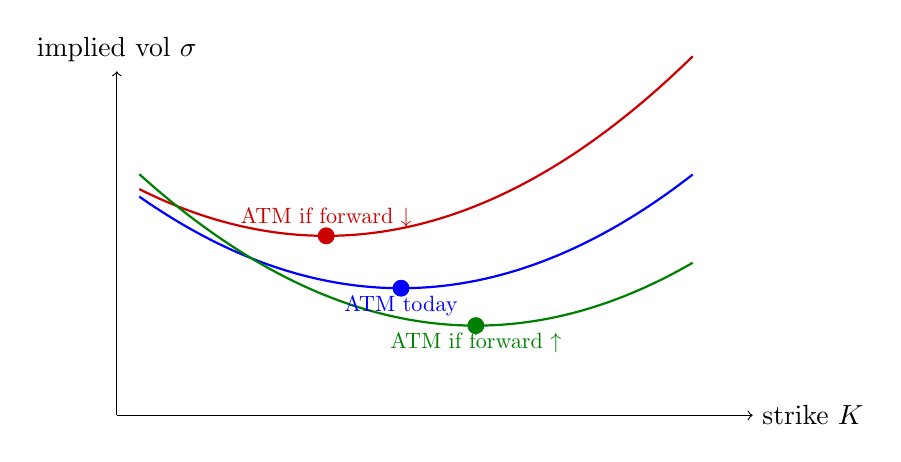
\begin{tikzpicture}[scale=0.95]
  \draw[->] (0,0) -- (8.5,0) node[right] {strike $K$};
  \draw[->] (0,0) -- (0,4.6) node[above] {implied vol $\sigma$};
  % Three smile curves: blue (today), red (forward down), green (forward up)
  \draw[thick,blue,smooth,domain=0.3:7.7,samples=100,variable=\x]
    plot ({\x},{ 1.7 + 0.10*((\x-3.8)*(\x-3.8)) });
  \draw[thick,red!80!black,smooth,domain=0.3:7.7,samples=100,variable=\x]
    plot ({\x},{ 2.4 + 0.10*((\x-2.8)*(\x-2.8)) });
  \draw[thick,green!50!black,smooth,domain=0.3:7.7,samples=100,variable=\x]
    plot ({\x},{ 1.2 + 0.10*((\x-4.8)*(\x-4.8)) });
  % ATM dots
  \filldraw[blue]       (3.8,1.70) circle (3pt) node[below,scale=0.8] {ATM today};
  \filldraw[red!80!black] (2.8,2.40) circle (3pt) node[above,scale=0.8] {ATM if forward $\downarrow$};
  \filldraw[green!50!black] (4.8,1.20) circle (3pt) node[below,scale=0.8] {ATM if forward $\uparrow$};
\end{tikzpicture}
\end{center}
\end{keyblock}

The lecturer's point: ``If I pull up my Bloomberg screen on ATM vol,
it's going to have jumped not from here to here vertically, it's
going to have jumped from the blue dot to the green dot.'' The
journalist headline (``ATM vol fell today'') fuses two distinct
things: where on the strike axis ATM is today, and which curve we
are sitting on. SABR makes that fusion explicit and sometimes
predicts that on \emph{your} inventory --- which is at a fixed strike,
not at ATM --- vol \emph{rose} even when the headline ATM number
fell. ``On my inventory, I'm going here from blue to orange. But if
I'm just taking the vol path, that headline number, I'm going from
where blue intersects the solid black to where orange intersects the
kind of dotted line.''

\subsection{Where SABR is the natural choice, and where it isn't}\label{L8-sec:whererates}

A student asked the natural follow-up: \emph{why} does SABR work
better for fixed-income derivatives than for, say, crude oil or
equities? The lecturer's answer was empirical, not theoretical:

\begin{quote}
\emph{Lecturer:} ``Is there a theoretical reason that SABR works
better for fixed income derivatives than, for example, crude oil or
equities? Or is it just empirically observed? \ldots\ It is largely
empirically observed. The choice of model in any of these markets
is made knowing how that market empirically tends to behave. For
equities, you see a lot of mean-reversion in volatility and the
implied-vol surface, so Heston-type models tend to dominate. SABR
can be used on equities, but it's not done much. SABR is the
workhorse for fixed-income derivatives because that's where the
empirical dynamics --- the $\rho < 0$ correlation, the $\beta$ near
$0.7$, the moderate $\nu$ --- happen to fit best. Sometimes useful
for FX. Mostly a curve-fitting tool for crude.''
\end{quote}

\begin{keyblock}
\textbf{The market-by-market verdict.}
\begin{itemize}
  \item \textbf{SOFR / Treasury / swaptions:} SABR is the market
        standard. Both static skew and dynamic skew-shifting predict
        well.
  \item \textbf{FX options:} SABR is sometimes used; alternatives
        include Vanna-Volga and stochastic-vol-with-jumps models.
  \item \textbf{Equities (SPX, ES):} SABR rarely used; Heston and
        local-vol-Heston blends dominate. Vol skew has too much
        mean-reversion structure for SABR's three parameters.
  \item \textbf{Crude oil:} SABR is sometimes fit for the curve
        shape but lecturer would not endorse the implied dynamics.
\end{itemize}
The principle: \emph{the modeling choice is calibrated to the
empirical regularities of the market}, not derived from first
principles.
\end{keyblock}

\subsection{The April 2025 SOFR-futures observations}\label{L8-sec:apr25}

The lecturer chose April 2025 as the case-study window because of
the tariff news cycle that month --- a window where rates
expectations were jumping around enough to test SABR's dynamic
content. ``I was just interested in whether we'd see something
here.''

\begin{keyblock}
\textbf{Cell~25 (Page \emph{SABR Skews for Futures} --- Other Assets).}
\emph{(How the comparison was structured.)}\\
For each business date in April 2025, fit SABR to that day's option
chain. Then compute the day-over-day change predicted by SABR
(based on the realized change in the forward rate and SABR's fitted
parameters from the prior day). Compare against the actual day-over-
day change. Report the cross-correlation of predicted-vs-actual
across the date panel and across strikes.
\end{keyblock}

The headline result the lecturer presented: predicted-vs-actual
correlation of about $80\%$, slope-coefficient on a regression of
actual on predicted of around $0.6$ to $0.7$ rather than $1$. So
SABR captures the direction and a substantial chunk of the day-to-day
dynamics, but the magnitude is over-predicted. ``If you let me just
fit my own line through here, it would say, take the SABR
predictions. Don't take them quite so seriously on the exact
scaling. But they really are lining up quite well in the
correlation.''

\subsection{The fit-grid and the case-study questions}\label{L8-sec:fitgrid}

\begin{keyblock}
\textbf{Cell~27 (Page \emph{SABR Skews for Futures} --- code).}
\emph{(The estimation loop.)}\\
For each date $i$ in the panel and each $\beta$ on a small grid
$\{0.5, 0.7, 0.9\}$, call
\begin{center}
\texttt{sabr\_volpaths(LOADFILE, i, ISCALL, beta, date\_t, shiftsize)}
\end{center}
and stash the per-day fitted $(\alpha, \rho, \nu)$ and the residual
fit metric. Iterate over strikes for the predicted-vs-actual table.
\end{keyblock}

The lecturer flagged \emph{three} layered choices the case study
deliberately avoids resolving. Most narrowly, what value of $\beta$
to fix --- $0.5$, $0.7$, $0.9$? The data weakly prefers something in
the middle but does not pin it down. Stepping out, is one day's
SABR fit representative? On some days the fitted $\rho$ is sharply
negative, on others nearly zero. Stepping out further, is SABR even
the right model for the product? The case study answers the third
question only for SOFR (yes) and rules it out for equities; the
others are left as ``it depends.''

\begin{checkpoint}
\textbf{My note.} The three-level question structure (parameter
choice $\to$ day-to-day stability $\to$ model adequacy) is a useful
review pattern for any calibration exercise on the exam. The same
ladder applies to Nelson--Siegel for the spot curve, to Black for
caplets, and to SABR here. Each level pushes the test harder: a
``good fit'' at level~1 means very little if level~3 fails. The
lecturer's case-by-case verdict (yes-SOFR, no-equity, maybe-FX) is a
level-3 statement and is the one a desk actually has to defend.
\end{checkpoint}

After the SABR-for-futures case the lecturer paused for a 12-minute
break and then turned to the second half of the lecture: numerical
methods.

\section{Numerical methods: where binomial trees fit}\label{L8-sec:nmframe}

The lecturer opened Chapter~9 with an explicit caveat about scope.
``This session, Chapter~9, is meant to be somewhat shorter because
it's really opening up things that would take a whole course\ldots\
I'm wary of doing anything where we just do a worse, faster version
of what we do in FinMath~320.'' The chapter therefore reads as a
\emph{landmark tour} rather than a self-contained development. Three
families of methods sit on the option-pricing pricing menu:

\begin{keyblock}
\textbf{The pricing-method menu.}
\begin{center}
\small
\begin{tabular}{l|l|l}
\textbf{Dynamics} & \textbf{Contract structure} & \textbf{Method} \\
\hline
simple (lognormal) & vanilla European & closed form (Black) \\
simple             & American / Bermudan & \emph{tree} \\
complex (jumps)    & vanilla            & finite difference / FFT \\
complex            & path-dependent     & Monte Carlo \\
\end{tabular}
\end{center}
\end{keyblock}

The lecturer wanted us to remember that trees occupy a specific
quadrant: \emph{simple} dynamics (essentially still log-normal, with
the diffusion approximated discretely) but \emph{complex} contract
structure --- the early-exercise feature of an American option,
the issuer's call right inside a callable bond, the prepayment
optionality in a mortgage-backed security. For everything in this
quadrant the tree's backward-induction algorithm handles optionality
``for free'' at each node. We will not in this lecture build the
machinery for jumps or path-dependent payoffs --- those are FinMath
320's territory --- but we will see the entire tree mechanic for the
fixed-income case.

\begin{tipblock}
\textbf{Filling the gap.} ``Why a \emph{tree} for an American option,
and why does Black not work?'' Black's formula assumes the holder
exercises optimally at expiration $T$ and only at $T$ --- the value
of the option is $Z(0,T)$ times the risk-neutral expectation of the
terminal payoff. An American option lets the holder exercise at any
date $t \le T$. At each $t$, the option's value is
\[
  V_t \;=\; \max\bigl(\,\text{intrinsic value at }t,\ \text{continuation value at }t\,\bigr),
\]
where ``continuation value'' is the discounted risk-neutral
expectation of $V_{t+\Delta t}$. There is no closed form for this
recursion in general --- but \emph{a tree solves it node by node,
backward in time, exactly}. That is the algorithmic contribution.
\end{tipblock}

\subsection{What this lecture will not cover}\label{L8-sec:notcover}

\begin{keyblock}
\textbf{Out of scope (and which course covers each).}
\begin{itemize}
  \item Calibration of an arbitrage-free rate tree to today's
        discount curve \emph{and} caplet vols simultaneously --- the
        full ``Black--Derman--Toy'' or ``Ho--Lee'' algorithm. (FINM
        37500 / FinMath 320.)
  \item Continuous-time short-rate models (Vasicek, CIR, Hull--White)
        and their tree counterparts. (FinMath 330.)
  \item LIBOR Market Model / SABR-LMM in practice. (FINM 37500 in a
        hypothetical 100-unit version.)
  \item Monte Carlo for path-dependent fixed-income payoffs.
        (FinMath 320.)
  \item Trinomial trees and explicit finite-difference schemes.
        (FinMath 320.)
\end{itemize}
\end{keyblock}

The lecturer wanted us to leave the lecture knowing what we don't
yet know, so that an exam answer or a desk question that wanders into
this territory triggers the right ``out of scope'' flag rather than
a guess.

\section{The equity binomial tree (one period)}\label{L8-sec:eqone}

The lecturer set up the binomial tree on the simplest example: a
single period, zero interest rate, two states. The deliberate choice
was to make the algebra trivial so that the \emph{logic} of
replication is in the foreground, not the bookkeeping.

\subsection{The setup}\label{L8-sec:setup}

\begin{keyblock}
\textbf{Cell (Page \emph{Intro to Binomial Trees}, Setup).}
\emph{(One period of uncertainty: $t = 0$ and $t = T$, no trading
in between, zero interest rate, stock either up or down.)}
\begin{center}
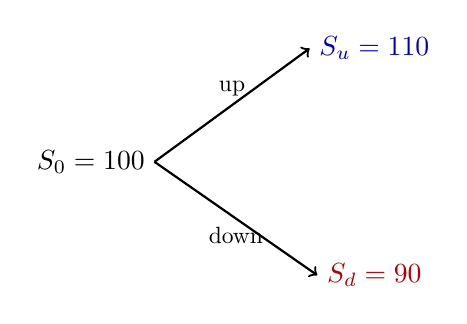
\begin{tikzpicture}[scale=1.2]
  \node (s0) at (0,0) {$S_0 = 100$};
  \node[blue!70!black] (su) at (3,1.2) {$S_u = 110$};
  \node[red!70!black] (sd) at (3,-1.2) {$S_d = 90$};
  \draw[->,thick] (s0.east) -- (su.west) node[midway,above,scale=0.85] {up};
  \draw[->,thick] (s0.east) -- (sd.west) node[midway,below,scale=0.85] {down};
\end{tikzpicture}
\end{center}
\textbf{The contract:} European call, strike $K = 105$, expiration $T$.
\[
  C_u \;=\; \max(S_u - K, 0) \;=\; \max(110 - 105, 0) \;=\; 5,
\]
\[
  C_d \;=\; \max(S_d - K, 0) \;=\; \max(90 - 105, 0) \;=\; 0.
\]
We do not assume any probability for the up-move. We will price $C_0$
without using one.
\end{keyblock}

The lecturer's framing here was deliberate. ``Notice we have not
talked about the probability of the up move. We will not need it.
This is the punchline of the binomial tree the same way it was the
punchline of Black's formula.'' The setup is structured so that
no-arbitrage replication will pin down the call price uniquely, with
no statement about how likely up is.

\subsection{The hedge ratio}\label{L8-sec:hedge}

\begin{keyblock}
\textbf{Hedge ratio (delta).} The number of shares of stock that
moves dollar-for-dollar with the call across the two states is
\[
  \Delta \;=\; \frac{C_u - C_d}{S_u - S_d}.
\]
Plugging in the numbers:
\[
  \Delta \;=\; \frac{5 - 0}{110 - 90} \;=\; \frac{5}{20} \;=\; 0.25.
\]
\end{keyblock}

The lecturer pushed the class to feel why this is the right number
before deriving anything. ``If the stock moves \$20 between up and
down, and the option moves \$5, then \$1 of stock is worth a quarter
of a dollar of option in this discrete world. So $0.25$ shares of
stock matches one short call.'' The hedge ratio is the ``coverage
ratio'' for moving dollar-for-dollar with the call.

\begin{tipblock}
\textbf{Filling the gap.} Why does the formula above give the
\emph{unique} hedge ratio that makes a long-stock-short-call
position riskless across the two states? Set up the riskless
condition explicitly. Suppose we hold $\Delta$ shares of stock and
short one call. The portfolio value at $T$ is
\[
  V_u \;=\; \Delta\,S_u - C_u, \qquad V_d \;=\; \Delta\,S_d - C_d.
\]
Riskless means $V_u = V_d$:
\[
  \Delta\,S_u - C_u \;=\; \Delta\,S_d - C_d
  \quad\Longleftrightarrow\quad
  \Delta\,(S_u - S_d) \;=\; C_u - C_d
  \quad\Longleftrightarrow\quad
  \Delta \;=\; \frac{C_u - C_d}{S_u - S_d}.
\]
That is the unique hedge ratio that turns the two-state portfolio
into one number across both branches.
\end{tipblock}

\subsection{Replicating the call: portfolio composition}\label{L8-sec:replicate}

With $\Delta = 0.25$, we go long $0.25$ shares of stock and short
one call. The terminal portfolio value is the same in both states:

\begin{keyblock}
\textbf{Cell~7 (Page \emph{Intro to Binomial Trees}, Replicating
Cash).}
\begin{align*}
  \text{UP:}\quad   V_u &\;=\; (0.25)(110) - 5 \;=\; 27.5 - 5 \;=\; 22.5, \\
  \text{DOWN:}\quad V_d &\;=\; (0.25)(90)  - 0 \;=\; 22.5 \;=\; 22.5.
\end{align*}
The portfolio pays \$22.50 at $T$ in both states. With the interest
rate at zero, the present value of this guaranteed cashflow is
\$22.50.
\end{keyblock}

\subsection{Pricing by no-arbitrage}\label{L8-sec:pricena}

Now use no-arbitrage. The cost of setting the portfolio up at
$t = 0$ must equal its (deterministic) terminal value of \$22.50
(with $r = 0$, the discount factor is $1$). Writing the cost in
terms of the position sizes,
\[
  V_0 \;=\; \Delta\,S_0 - C_0
       \;=\; 0.25 \cdot 100 - C_0
       \;=\; 25 - C_0,
\]
and setting $V_0 = 22.5$ solves for the call's price:
\[
  C_0 \;=\; 25 - 22.5 \;=\; 2.50.
\]

The lecturer dwelt on the no-arbitrage move. ``Why must the cost of
setting up this portfolio equal \$22.50? Because the portfolio's
final payoff is \$22.50 with certainty, in either state. If you
could buy the portfolio for less than \$22.50, you would lock in a
risk-free profit of (\$22.50 minus what you paid). If you could
short the portfolio for more than \$22.50, you would short at the
high price, repay \$22.50 at $T$, and pocket the difference. Since
neither arbitrage exists, the cost is forced to be \$22.50.'' That
is the entire pricing argument; the algebra solves for $C_0 = 2.50$.

\section{The risk-neutral interpretation of $p^*$}\label{L8-sec:rnpstar}

The same answer falls out of a re-interpretation that will scale to
multiperiod trees and to interest-rate trees: the risk-neutral
formulation.

\subsection{The pricing formula}\label{L8-sec:priceformula}

\begin{keyblock}
\textbf{Cell~13 (Pricing Formula).}
The cost of setting up the riskless portfolio is $S_0\,\Delta - C_0$
and its present value of the guaranteed payoff is $S_u\,\Delta - C_u$
(any state would do --- they are equal). Setting them equal and
solving for $C_0$:
\[
  C_0 \;=\;
    C_u\,\underbrace{\,\frac{S_0 - S_d}{S_u - S_d}\,}_{p^*}
    \;+\;
    C_d\,\underbrace{\,\frac{S_u - S_0}{S_u - S_d}\,}_{1 - p^*}.
\]
The numbers $p^*$ and $1 - p^*$ depend only on the stock-tree
geometry $(S_0, S_u, S_d)$, not on $K$ or any payoff. With our
numbers, $p^* = (100 - 90)/(110 - 90) = 0.5$, and indeed
$0.5 \cdot 5 + 0.5 \cdot 0 = 2.5$.
\end{keyblock}

\begin{tipblock}
\textbf{Filling the gap.} The algebra from the riskless equality
$S_0\,\Delta - C_0 = (S_u\,\Delta - C_u)\,Z$ where $Z$ is the
discount factor and $\Delta = (C_u - C_d)/(S_u - S_d)$. Substituting,
\[
  S_0\,\frac{C_u - C_d}{S_u - S_d} - C_0 \;=\; Z\Bigl[S_u\,\frac{C_u - C_d}{S_u - S_d} - C_u\Bigr],
\]
and rearranging for $C_0$, multiplying through and grouping the $C_u$
and $C_d$ terms separately, gives
\[
  C_0 \;=\; Z\Bigl[\,C_u\,\frac{S_0/Z - S_d}{S_u - S_d}
                  + C_d\,\frac{S_u - S_0/Z}{S_u - S_d}\,\Bigr].
\]
With $r = 0$, $Z = 1$ and we get the displayed formula. With $r \ne 0$,
$Z = e^{-r\,\Delta t}$ and the inside fractions become
$p^* = (A\,S_0 - S_d)/(S_u - S_d)$ where $A = e^{r\,\Delta t}$. The
algebra is mostly bookkeeping; what matters is that $C_0$ is a
discounted weighted average of $C_u$ and $C_d$ with weights that
\emph{do not depend on the call's payoffs}.
\end{tipblock}

\subsection{Three ways to read $p^*$}\label{L8-sec:threereads}

\begin{keyblock}
\textbf{Cell~16 (Probability interpretation).}
Read $p^*$ as a ``probability'' of the up-state. Then
\[
  C_0 \;=\; p^* \cdot C_u + (1 - p^*)\cdot C_d \;=\; \E^{*}[C_T],
\]
where $\E^{*}$ is expectation under that probability. With our
numbers, $p^* = 0.5$, $C_0 = \E^{*}[C_T] = 0.5 \cdot 5 + 0.5 \cdot 0 = 2.5$,
which is exactly the price.
\end{keyblock}

The lecturer was emphatic: $p^*$ is \emph{not} the true probability
of the up-state. ``We never used the true probability anywhere in
this derivation. The $p^*$ falls out of the geometry of the stock
tree --- $S_0$, $S_u$, $S_d$ --- via no-arbitrage. We \emph{label}
it a probability because the formula has the shape of an expected
value, and that label is going to be a powerful organizing device.
But $p^*$ is a pricing object, not a forecast.''

\begin{keyblock}
\textbf{Cell~17 (State-contingent payoffs).}
A second reading: define $U$ and $D$ to be the time-zero prices of
\emph{state-contingent claims} that pay \$1 in the up state and \$0
otherwise (and vice versa). Any payoff $f$ at $T$ is a portfolio of
$U$'s and $D$'s:
\[
  f(\omega) \;=\; f_u\cdot \mathbf{1}_{\{\omega = u\}} + f_d \cdot \mathbf{1}_{\{\omega = d\}}.
\]
Its time-zero price is therefore $f_u \cdot P_U + f_d \cdot P_D$,
where $P_U$ and $P_D$ are the prices of $U$ and $D$. In the zero-rate
single-period example, $P_U = p^*$, $P_D = 1 - p^*$, recovering
the formula.
\end{keyblock}

\begin{checkpoint}
\textbf{My note.} The state-price reading is the one that
generalizes most cleanly. In a multiperiod tree (or a continuous
model), every node carries a state-price; pricing any payoff is just
a weighted sum of these prices over the payoff support. The
``risk-neutral expectation'' phrasing is a compact rewording. I
expect the exam to lean on the no-arbitrage replication argument,
since that is what pins down the prices uniquely; the
risk-neutral and state-price readings are equivalent ways to
compute.
\end{checkpoint}

\subsection{Key features of the binomial pricing solution}\label{L8-sec:keyfeatures}

\begin{keyblock}
\textbf{Cell~18 (Key features).}
\begin{itemize}
  \item We priced the call without ever knowing the actual tree
        probabilities.
  \item In this simple tree, ``not knowing the true probabilities''
        is equivalent to ``not knowing the stock's drift'' --- the
        call's price is independent of the drift.
  \item The hedge ratio $\Delta$ is constructive: it tells us the
        portfolio that replicates the call.
  \item Replication ties the price to existing tradeables ($S$ and
        cash), not to a model.
\end{itemize}
\end{keyblock}

The lecturer emphasized the independence of price from drift as
the binomial-tree analogue of Black's most counterintuitive result.
``Black's formula doesn't have $\mu$ in it. Why? For exactly the
same reason this tree doesn't need the up-probability: the
replication argument doesn't care what you think the drift is. You
either replicate the option or you don't. If you do, the price is
pinned down by what you can already trade.''

\section{Generalizing the binomial tree}\label{L8-sec:general}

The lecturer next walked through the upgrades needed to take this
single-period zero-rate equity tree and turn it into a usable
machine. Each upgrade is small; the cumulative effect is a tree
that handles real-world derivatives.

\subsection{General notation}\label{L8-sec:gennotation}

\begin{keyblock}
\textbf{Cell~22--25 (General notation).}
For a generic underlying $S$ over a time interval $\Delta t$,
\[
  S_u \;=\; u\,S_0,
  \qquad
  S_d \;=\; d\,S_0,
\]
with $u > 1 > d > 0$ multiplicative ``up'' and ``down'' factors. The
derivative price is denoted $f$ (call, put, or any other contract).
The continuously compounded interest rate over $\Delta t$ is $r$, and
\[
  Z \;=\; e^{-r\,\Delta t}, \qquad A \;=\; e^{r\,\Delta t}, \qquad Z = 1/A.
\]
The risk-neutral up-weight becomes
\[
  p^* \;=\; \frac{A - d}{u - d},
\]
and the no-arbitrage pricing formula becomes
\[
  f_0 \;=\; Z\Bigl[\,p^*\,f_u + (1 - p^*)\,f_d\,\Bigr].
\]
\end{keyblock}

The form is identical to the zero-rate case except for the discount
factor $Z$ in front and the $A = e^{r\,\Delta t}$ growth factor inside
$p^*$. ``All we did was put discounting back in. Nothing structural
changed.''

\subsection{Setting $u$ and $d$: matching volatility}\label{L8-sec:vol}

The next question is parametric: how do we choose $u$ and $d$? The
lecturer's slide gave the standard answer:

\begin{keyblock}
\textbf{Cell~30 (Setting $u$ and $d$ via volatility).}
The variance of one step (a Bernoulli with up-probability the true,
\emph{not risk-neutral}, probability) is computed in
log-returns. Match it to the variance of a continuous-time
log-normal process with volatility $\sigma$ over $\Delta t$:
\[
  \Var\bigl(\,\ln(S_T/S_0)\,\bigr) \;=\; \sigma^2 \,\Delta t.
\]
The Cox--Ross--Rubinstein (CRR) choice that solves this with
$ud = 1$ is
\[
  u \;=\; e^{\sigma\sqrt{\Delta t}},
  \qquad
  d \;=\; e^{-\sigma\sqrt{\Delta t}}.
\]
\end{keyblock}

\begin{tipblock}
\textbf{Filling the gap.} Why $ud = 1$ as a side-condition, and why
that closed form? Two equations are needed to pin down $u$ and $d$:
volatility match (one equation) plus a symmetry condition (the
second). $ud = 1$ is the recombining-tree condition --- after one
up and one down, the tree returns to $S_0$ --- which keeps the
multiperiod tree small (size grows linearly with depth, not
exponentially). With $ud = 1$, $d = 1/u$. Substituting into the
volatility-match equation and solving gives the
$u = e^{\sigma\sqrt{\Delta t}}$, $d = e^{-\sigma\sqrt{\Delta t}}$
formulas above. Other choices --- Jarrow-Rudd, Tian's --- correspond
to different second conditions and different $u$, $d$ pairs, but
CRR is the standard for fixed-income work.
\end{tipblock}

\subsection{Adjusting $A$ for dividends and futures}\label{L8-sec:adjustA}

\begin{keyblock}
\textbf{Cell~31 (Other settings).}
The growth factor $A$ depends on what the underlying is:
\[
  A \;=\;
    \begin{cases}
      e^{r\,\Delta t} & \text{non-dividend stock,} \\
      e^{(r - q)\,\Delta t} & \text{stock with continuous dividend yield } q, \\
      1               & \text{futures contract,} \\
      e^{(r - r_f)\,\Delta t} & \text{currency, with foreign rate } r_f.
    \end{cases}
\]
The pricing recursion $f_0 = Z\,[\,p^* f_u + (1-p^*) f_d\,]$ is
unchanged --- only the input $A$ inside $p^*$ shifts.
\end{keyblock}

The futures case is the one we will need for SOFR-futures option
pricing. ``Futures contracts have no carrying cost, so the expected
move under the risk-neutral measure is zero --- $A = 1$. Plug
$A = 1$ into $p^* = (A - d)/(u - d) = (1 - d)/(u - d)$ and the rest
of the machinery is unchanged.''

\subsection{Two concerns: market incompleteness and time discretization}\label{L8-sec:concerns}

\begin{keyblock}
\textbf{Cell~32 (Concerns).}
\begin{itemize}
  \item \textbf{Market incompleteness from discretization of space.}
        With only two states, every claim is replicable by the
        riskless portfolio of $S$ and cash. With three or more
        states, the same machinery breaks: not every payoff is
        replicable, $p^*$ is not unique, and no-arbitrage gives a
        \emph{range} of consistent prices, not a single price.
  \item \textbf{Time discretization.} The continuous-time process
        is being approximated by a discrete tree. As $\Delta t \to 0$
        with the volatility-matching $u, d$, the tree's distribution
        of $\ln S_T$ converges to the lognormal --- but at any
        finite $\Delta t$, it is an approximation.
\end{itemize}
\end{keyblock}

The lecturer let the second concern pass quickly --- ``in practice
you take 30 steps for a vanilla American, more for an exotic, the
convergence is fine.'' The first concern is the deeper one and
deserves a tipblock.

\begin{tipblock}
\textbf{Filling the gap.} What does ``three states break replication''
mean concretely? Suppose the stock can go to $S_u$, $S_m$, $S_d$
with $S_d < S_m < S_u$, and we want to price a call. We have two
tradeables (stock and cash) and three states. The hedge equation
$\Delta\,S_x - C_x = V$ (with $V$ a constant) is one equation per
state, three in total, but only two unknowns ($\Delta, V$ together
with the requirement that the cost-of-setup match). Three equations,
two unknowns: generically no solution. The market-completeness
condition for replication is
\[
  \#\{\text{tradeable assets}\} \;\ge\; \#\{\text{states}\}.
\]
A trinomial tree therefore is \emph{incomplete} unless one adds a
third tradeable (a second option, the bond market, etc). Pricing
inside a trinomial requires a richer machinery: a market price of
risk, or an explicit choice of the third tradeable.
\end{tipblock}

\section{From equities to interest rates}\label{L8-sec:rateequities}

The lecturer's next move was the one fixed-income students need to
internalize for the rest of the class. ``Apply the same principles
to a case where the underlying tree is not a traded security, but
rather \emph{interest rates}.''

\subsection{Why this is more delicate}\label{L8-sec:moredelicate}

\begin{keyblock}
\textbf{The crucial twist.} The interest rate $r$ is \emph{not}
itself a traded security. It is a quantity the bond market lets us
infer (via the discount curve), but you cannot ``buy a unit of the
short rate'' the way you can buy a share of stock. The replication
argument therefore needs a substitute for ``stock'' --- and the
substitute is \emph{bonds of various maturities}.
\end{keyblock}

The lecturer's framing: ``In the equity tree we replicated the call
using stock and cash. In the rate tree we will replicate the rate
option using a 1-period bond and a 2-period bond. The 1-period
bond plays the role of cash --- it pays a known amount at time
$\Delta t$. The 2-period bond plays the role of stock --- its time-
$\Delta t$ price is uncertain because rates have moved.''

\subsection{Setup: the rate tree}\label{L8-sec:ratetree}

\begin{keyblock}
\textbf{Cell~33--37 (Rate tree setup).}
Use $\Delta t = 0.5$ years (six-month tree step). At each node,
the rate is the continuously-compounded six-month rate prevailing
between the current node and the next. Equivalently, this is
\begin{itemize}
  \item the discount rate over the period, or
  \item the YTM on a six-month zero-coupon bond starting at the
        node.
\end{itemize}

\begin{center}
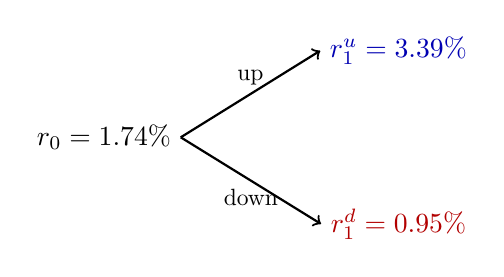
\begin{tikzpicture}[scale=1.1]
  \node (r0) at (0,0) {$r_0 = 1.74\%$};
  \node[blue!70!black] (ru) at (3.4,1.0) {$r_1^u = 3.39\%$};
  \node[red!70!black] (rd) at (3.4,-1.0) {$r_1^d = 0.95\%$};
  \draw[->,thick] (r0.east) -- (ru.west) node[midway,above,scale=0.85] {up};
  \draw[->,thick] (r0.east) -- (rd.west) node[midway,below,scale=0.85] {down};
\end{tikzpicture}
\end{center}
\textbf{Quotes used to build the tree.}
\begin{center}
\begin{tabular}{c|c|c}
\textbf{maturity (yrs)} & \textbf{price (per \$100)} & \textbf{YTM} \\
\hline
$0.5$ & $99.13$ & $1.74\%$ \\
$1.0$ & $97.89$ & $2.13\%$ \\
$1.5$ & $96.15$ & $2.62\%$ \\
\end{tabular}
\end{center}
\end{keyblock}

The numbers are deliberately small (only three nodes, only one
period of uncertainty) so the algebra in a moment is clean. The
key is that we have \emph{two bonds} (1-period maturing at
$\Delta t = 0.5$ and 2-period maturing at $1.0$) and \emph{two
states} of the rate at $\Delta t$.

\subsection{Why continuously compounded?}\label{L8-sec:contcompound}

\begin{keyblock}
\textbf{Cell~40 (Why continuous compounding).}
``This is miles vs kilometers, not a modeling choice. There is a
one-to-one mapping from continuous-compounding to any other
compounding convention. As we change the time-step of the tree, we
do not want to change all the compounding rates. The continuously-
compounded form is invariant to $\Delta t$ --- the same $r_0$
multiplies the same $\Delta t$ regardless of whether we cut the
tree into $0.5$-year or $0.25$-year steps. This will converge to
the continuous-time short-rate model as $\Delta t \to 0$.''
\end{keyblock}

The lecturer's point: a semi-annually-compounded rate would
need to be re-expressed every time we change $\Delta t$. With
continuous compounding the discount factor is always
$Z = e^{-r\,\Delta t}$ regardless of how finely we discretize, and
the limit as $\Delta t \to 0$ is exactly the continuous-time
short-rate model that fixed-income textbooks treat.

\section{Pricing a rate option (one period)}\label{L8-sec:rateoption}

\subsection{The contract}\label{L8-sec:contract}

\begin{keyblock}
\textbf{Cells~42--44 (rate option).}
A simple interest-rate option, treated by analogy to a put on a stock:
\begin{itemize}
  \item Payoff at period~$1$ ($t = \Delta t = 0.5$).
  \item Strike rate $r_K = 2\%$.
  \item Payoff: $100 \cdot \max(r_K - r_1, 0)$ per \$100 face.
\end{itemize}
With the rate tree above, $r_1^u = 3.39\%$ and $r_1^d = 0.95\%$:
\[
  f_u \;=\; 100\cdot\max(0.02 - 0.0339, 0) \;=\; 0,
  \qquad
  f_d \;=\; 100\cdot\max(0.02 - 0.0095, 0) \;=\; 1.05.
\]
\end{keyblock}

The contract is the simplest possible rate-floor-let: pay if the
rate falls below the strike. It will be the building block for the
floor-pricing exercise in Class~8.2.

\subsection{Replicating the rate option}\label{L8-sec:repl}

The crucial difference from the equity case: instead of replicating
with stock and cash, we replicate with the \emph{1-period} bond and
the \emph{2-period} bond.

\begin{keyblock}
\textbf{Cells~45--50 (replication portfolio).}
Let $\alpha$ be the position in the 1-period bond and $\beta$ the
position in the 2-period bond. The 1-period bond is risk-free over
the step ($t = 0$ to $t = \Delta t$): it matures at \$100 face.
The 2-period bond's time-$\Delta t$ price is uncertain because it
still has one period left and the rate is now $r_1$:
\[
  P^{(2)}_u \;=\; 100/A^u \;=\; 98.32,
  \qquad
  P^{(2)}_d \;=\; 100/A^d \;=\; 99.53,
\]
where $A^u = e^{r_1^u \,\Delta t}$ and similarly for $d$. Match the
call payoff state-by-state:
\[
  \alpha \cdot 100 + \beta \cdot P^{(2)}_u \;=\; f_u \;=\; 0,
  \qquad
  \alpha \cdot 100 + \beta \cdot P^{(2)}_d \;=\; f_d \;=\; 1.05.
\]
\end{keyblock}

This is two equations in two unknowns. Subtracting the first from
the second:
\[
  \beta\,(P^{(2)}_d - P^{(2)}_u) \;=\; f_d - f_u
  \quad\Longleftrightarrow\quad
  \beta \;=\; \frac{f_d - f_u}{P^{(2)}_d - P^{(2)}_u}.
\]
Plugging back into the first equation gives $\alpha$. Numerically:
\[
  \beta \;=\; \frac{1.05 - 0}{99.53 - 98.32} \;=\; \frac{1.05}{1.21}
       \;\approx\; 0.868,
  \qquad
  \alpha \;=\; \frac{f_u - \beta\,P^{(2)}_u}{100} \;\approx\; -0.853.
\]

\begin{tipblock}
\textbf{Filling the gap.} Why does the 2-period bond play the role
of ``stock'' in this replication? Because its time-$\Delta t$ price
is uncertain. The 1-period bond is known (it matures and pays \$100).
The 2-period bond, by contrast, has one period of uncertainty left
in it; its price moves with the rate. So the analogy is:

\begin{center}
\begin{tabular}{l|l|l}
\textbf{Equity tree} & \textbf{Rate tree} & \textbf{Role} \\
\hline
stock $S$              & 2-period bond $P^{(2)}$ & risky asset \\
cash (constant 1)      & 1-period bond $P^{(1)} = 100$ & riskless asset \\
call $C$               & rate option $f$         & contingent claim
\end{tabular}
\end{center}

The replication algebra is structurally identical; only the
underlyings have changed.
\end{tipblock}

\subsection{Pricing by no-arbitrage}\label{L8-sec:rateprice}

\begin{keyblock}
\textbf{Pricing the rate option.}
The cost at $t = 0$ of the replicating portfolio is
\[
  f_0 \;=\; \alpha \cdot P^{(1)}_0 + \beta \cdot P^{(2)}_0
       \;=\; \alpha \cdot 99.13 + \beta \cdot 97.89.
\]
With $\alpha \approx -0.853$ and $\beta \approx 0.868$,
$f_0 \approx 0.34$ per \$100 face.
\end{keyblock}

\subsection{Risk-neutral check}\label{L8-sec:rncheck}

\begin{keyblock}
\textbf{Cells~54--56 (risk-neutral pricing of the rate option).}
The risk-neutral probability satisfies (using the 2-period bond as
the underlying)
\[
  p^* \;=\;
    \frac{A\,P^{(2)}_0 - P^{(2)}_d}{P^{(2)}_u - P^{(2)}_d},
\]
where $A = e^{r_0\,\Delta t}$. Once $p^*$ is computed, pricing any
contingent claim on the rate is the discounted risk-neutral
expectation:
\[
  f_0 \;=\; Z\bigl[\,p^* \,f_u + (1 - p^*)\,f_d\,\bigr].
\]
The two routes (replication and risk-neutral) give the same price.
\end{keyblock}

\begin{checkpoint}
\textbf{My note.} The replication and the risk-neutral readings
again coincide because the rate-tree market with two bonds and two
states is complete. Any contingent claim on $r_1$ can be replicated
by a portfolio of the 1-period and 2-period bonds. The lecturer
emphasized this is the ``why'' for using \emph{two} bonds in the
replication: with only one bond the rate market would be incomplete
and pricing would not be unique. The 2-period bond contributes the
price-uncertainty that the rate option has exposure to.
\end{checkpoint}

\subsection{Independence from drift}\label{L8-sec:noDrift}

\begin{keyblock}
\textbf{Cell~64 (true probability vs risk-neutral).}
By Girsanov's theorem the true expectation and the risk-neutral
expectation are linked by a Radon--Nikodym factor whose log-derivative
contains the \emph{market price of (the underlying) risk}. The
crucial consequence: $f_0$ is independent of the true probability
of the up-state. The pricing equation depends only on the bond-
tree geometry $(P^{(2)}_0, P^{(2)}_u, P^{(2)}_d)$ via $p^*$ and on
the option payoffs $f_u, f_d$. We never needed to know the true
probability of the rate going up tomorrow.
\end{keyblock}

The lecturer was emphatic about this. ``All of the discussion you
hear from the Fed and from the FOMC about whether rates are going
to go up tomorrow has \emph{nothing} to do with the price of an
interest-rate derivative today. It only enters through what people
have already paid for the 2-period bond. Once that price is in,
the option's price is pinned down.'' This is the same drift-
independence we saw in the equity binomial and in Black: replication
arguments do not need the drift.

\section{The multiperiod tree}\label{L8-sec:multiperiod}

\subsection{Recap of the one-period structure}\label{L8-sec:oneprecap}

\begin{keyblock}
\textbf{Cell~66 (Reminder).}
The one-period tree has handed us:
\begin{itemize}
  \item A \textbf{replication argument}: build a portfolio of
        underlying tradeables that matches the option's payoffs in
        every state; the no-arbitrage cost equals the option price.
  \item A \textbf{risk-neutral interpretation}: the price is a
        discounted weighted average of the option's terminal
        payoffs with weights $p^*$, $1 - p^*$ derived from the
        underlying tree.
  \item A \textbf{drift-independence}: the answer does not depend
        on the true probabilities of the up- and down-states.
\end{itemize}
The same structure carries over to multi-period trees, applied
recursively.
\end{keyblock}

\subsection{Building the multiperiod tree}\label{L8-sec:multitree}

\begin{keyblock}
\textbf{Cell~67--70 (multiperiod tree).}
Continue the equity tree to a second period:
\begin{itemize}
  \item Apply $u$ and $d$ at every node so that
        $S_{0}\,uu \cdot ud \cdot du \cdot dd$ are the terminal
        states. With $ud = 1$ (CRR), the tree
        \emph{recombines}: $S_0\,ud = S_0\,du = S_0$, so after one
        up and one down we are back at $S_0$. The tree at depth $n$
        has $n + 1$ terminal nodes (linear in depth, not
        exponential).
  \item Use the contract to compute the payoff at each terminal node.
  \item \textbf{Move backward.} At each penultimate node, run a
        one-period tree with the two children to get the option
        value at that node. ``We have two separate, one-period
        trees. The solution procedure works exactly as discussed
        before --- same formulas, with the obvious adaptations.
        $f_{uu}$ and $f_{ud}$ instead of $f_u$ and $f_d$. $S_0\,uu$
        and $S_0\,ud$ instead of $S_u$ and $S_d$.''
  \item Repeat until reaching the root.
\end{itemize}
\end{keyblock}

\begin{center}
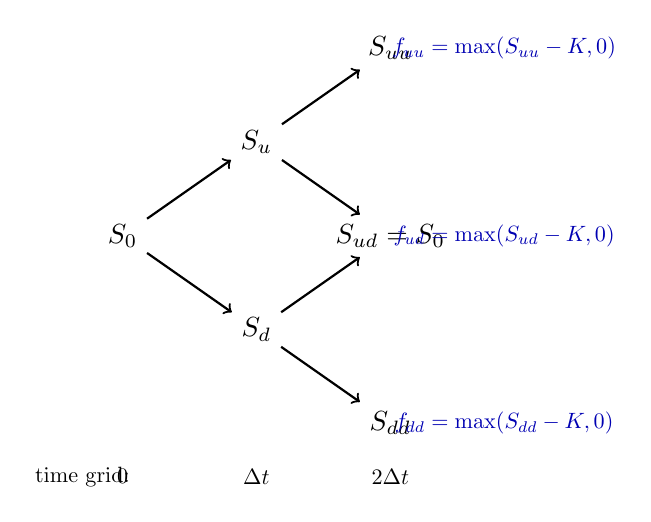
\begin{tikzpicture}[scale=0.85]
  % Multiperiod CRR recombining tree at depth 3
  \node (s0) at (0,0) {$S_0$};
  \node (su) at (2,1.4) {$S_u$};
  \node (sd) at (2,-1.4) {$S_d$};
  \node (suu) at (4,2.8) {$S_{uu}$};
  \node (sud) at (4,0)   {$S_{ud}=S_0$};
  \node (sdd) at (4,-2.8) {$S_{dd}$};
  \draw[->,thick] (s0) -- (su);
  \draw[->,thick] (s0) -- (sd);
  \draw[->,thick] (su) -- (suu);
  \draw[->,thick] (su) -- (sud);
  \draw[->,thick] (sd) -- (sud);
  \draw[->,thick] (sd) -- (sdd);
  \node[scale=0.8,blue!70!black] at (5.7,2.8)   {$f_{uu}=\max(S_{uu}-K,0)$};
  \node[scale=0.8,blue!70!black] at (5.7,0)     {$f_{ud}=\max(S_{ud}-K,0)$};
  \node[scale=0.8,blue!70!black] at (5.7,-2.8)  {$f_{dd}=\max(S_{dd}-K,0)$};
  \node[scale=0.8] at (-0.6,-3.6) {time grid:};
  \node[scale=0.8] at (0,-3.6) {$0$};
  \node[scale=0.8] at (2,-3.6) {$\Delta t$};
  \node[scale=0.8] at (4,-3.6) {$2\Delta t$};
\end{tikzpicture}
\end{center}

The picture is the standard CRR recombining tree at depth $n = 2$.
At depth $n$ in general, the tree has $n + 1$ terminal nodes; the
total number of nodes (including all interior ones) is $\binom{n+2}{2}
= O(n^2)$. Backward induction at each interior node is one
``one-period tree'' computation. So the total cost is also $O(n^2)$.

\subsection{Choosing the time grid}\label{L8-sec:timegrid}

\begin{keyblock}
\textbf{Cell~73 (choosing $\Delta t$).}
The time grid must be fine enough for the discrete tree's terminal
distribution to approximate the continuous-time lognormal
distribution well enough for the contract.
\begin{itemize}
  \item \textbf{Vanilla American:} around 30 steps is standard.
  \item \textbf{Bermudan / callable bonds:} 50--100 steps; the
        exercise dates need to align with tree time steps.
  \item \textbf{Exotic (barrier, knock-in):} hundreds of steps
        because the precise location of the barrier matters.
\end{itemize}
Too coarse $\Rightarrow$ the convergence error is large. Too fine
$\Rightarrow$ the computation slows down quadratically (depth $n$
gives $O(n^2)$ work for vanilla American payoffs, more for
path-dependent ones).
\end{keyblock}

\subsection{Specific underlying values: trinomial alternative}\label{L8-sec:trinomial}

\begin{keyblock}
\textbf{Cell~74 (specific underlying values).}
The CRR tree does not let us hit a specific terminal stock price
on the grid. We choose $u$ and $d$ to match volatility, and the
terminal nodes land at $S_0\,u^k\,d^{n-k}$ for $k = 0, \ldots, n$ ---
which prices we cannot pre-select. For some payoffs (a barrier at
exactly $S = 110$, say) we want the grid to pass through that price
exactly. \textbf{Trinomial trees} give that flexibility: at each
node the underlying can go up, down, or stay flat, with the third
parameter giving an extra degree of freedom to fix the grid points.
The tradeoff is market incompleteness in the trinomial (recall the
three-states-not-replicable argument), addressed by adding a third
tradeable to the replication.
\end{keyblock}

\begin{checkpoint}
\textbf{My note.} The trinomial / specific-grid issue is not on
the homework, but it is important to recognize as the reason the
binomial-tree machinery is not the only choice. For a SOFR-futures
option with a strike at exactly $4.25\%$, a trinomial with the grid
forced through $4.25\%$ at the option expiration node is more
accurate than a CRR binomial that happens to pass close to $4.25\%$
but not through it. The binomial's error in this case is
proportional to the distance from the nearest grid point to the
strike --- and that distance does not go to zero as
$\Delta t \to 0$ at the same rate as the volatility-matching error.
\end{checkpoint}

\section{Using binomial trees in practice}\label{L8-sec:usingbintrees}

After the break the lecturer ran through the operational use of a
calibrated rate tree, walking through the same notebook page
(\emph{Using Binomial Trees}) one cell at a time. The point of this
half-hour is not to derive new theory but to see the tree applied to
each fixed-income product the course has covered.

\subsection{The calibrated rate tree as a primitive}\label{L8-sec:ratetreeprim}

\begin{keyblock}
\textbf{Cell~7 (Page \emph{Using Binomial Trees}).}
\emph{(The rate tree, displayed.)}\\
\texttt{display\_bintree\_valuation(ratetree, refratetree, charttype='df',
title='Rates (compounding=\{freqcurve\})', fmt='\{:.1\%\}')}\\
The cell prints the rate tree as a triangular DataFrame: rows indexed
by tree node, columns indexed by time step. Each entry is the rate
prevailing in that state at that time. The lecturer emphasized that
this tree is the \emph{primitive} for everything that follows.
``This is just a tree of three-month interest rates --- annualized.
Once I have this, I can price any rate-dependent payoff.''
\end{keyblock}

The lecturer described the rate tree as ``the universal language''
for the tree-based half of fixed-income derivatives: every product
in the rest of the lecture is built on this same tree. The tree was
calibrated to today's discount curve at the level (so that
1-period, 2-period, ... bonds price correctly) and to today's caplet
volatilities (so that the dispersion across rows matches Black's
implied vols). The full calibration recipe --- Black-Derman-Toy or
Ho-Lee --- is the FinMath 320 / FINM 37500 material flagged earlier.

\subsection{Pricing a floor on the rate tree}\label{L8-sec:floortree}

\begin{keyblock}
\textbf{Cell~9 (Page \emph{Using Binomial Trees}, floor).}
\emph{(Pricing a 3-year, quarterly floor as a floorlet sum.)}
\begin{verbatim}
SECURITY = 'floor'
isPayer  = False
T        = 3
freq     = 4
output = bintrees(SECURITY, ratetree, curves, T=T,
                  cffreq=freq, isPayer=isPayer,
                  cmpnd_ratetree=CMPND_RATETREE)
\end{verbatim}
The function walks the tree backward, applying at each node the
floorlet payoff $\max(K - r_t, 0) \cdot \text{notional}$ when the
node is a reset date, then averaging weighted by $p^*$ and
discounting by the local rate.
\end{keyblock}

The lecturer's framing: ``A floor is a bundle of floorlets. At each
quarterly reset date, the floor pays
$\max(K - r_t, 0)$ on a fraction of the notional. The tree handles
each floorlet as one mini-payoff at the right node, and the
backward induction sums them with the right discount factors. So
the floor's price comes out as one number at the root --- a
weighted average of all the floorlets' state-by-state payoffs.''

\begin{keyblock}
\textbf{The mechanics displayed.}
For each terminal-state node (each leaf), compute
$\max(K - r_{\text{leaf}}, 0)$. At each interior node, set
\[
  V_{\text{node}}
   \;=\; Z_{\text{node}}\Bigl[\,
              p^*\,V_{\text{up child}} \;+\; (1 - p^*)\,V_{\text{down child}}
            + \mathbf{1}\{\text{node is a reset date}\}
            \cdot \max(K - r_{\text{node}}, 0)\Bigr].
\]
The discount $Z_{\text{node}} = e^{-r_{\text{node}}\,\Delta t}$. The
$p^*$ depends on the tree's geometry at the node. The price at the
root is the floor's value today.
\end{keyblock}

\begin{checkpoint}
\textbf{My note.} The recursion above looks more general than the
single-period one because it adds the per-node payoff term inside
the discounted expectation. That is the binomial-tree analog of
``intermediate cashflows go in the running discounted expectation''
which is how multi-period payoffs are integrated. For a vanilla
European call this term is zero except at the leaf; for an American
call we replace the first term inside the bracket with
$\max(\,p^*\,V_u + (1-p^*)\,V_d,\ \text{intrinsic}\,)$; for a floor
the floorlet-payoff term lights up at every reset date.
\end{checkpoint}

\subsection{European versus American swaption}\label{L8-sec:eurusdam}

\begin{keyblock}
\textbf{Cell~18--22 (Page \emph{Using Binomial Trees}, swaptions).}
For a swaption with European exercise, the algorithm is:
\begin{itemize}
  \item Build the underlying \emph{swap value tree} (the value of
        the underlying swap at each node).
  \item At expiration $T_o$, set $V_{\text{node}} =
        \max(\text{underlying swap value}, 0)$ (for a payer
        swaption; flip the sign for receiver).
  \item Backward-induct without intermediate exercise (no
        $\max$ at interior nodes).
\end{itemize}

\begin{verbatim}
output = bintrees(SECURITY, ratetree, curves, T=T, Topt=Topt,
                  undertree=valtrees['swap'], style=STYLE,
                  ivol=swapvol, cffreq=freq, isPayer=isPayer,
                  cmpnd_ratetree=CMPND_RATETREE)
valtrees['swaption european'] = output['tree value']
\end{verbatim}

For an American swaption (or Bermudan, with exercise restricted to
specific dates), replace the backward-induction step at each
exercise-eligible node with
\[
  V_{\text{node}}
    \;=\; \max\Bigl(\,
              \text{intrinsic at node},\ Z\,(\,p^* V_u + (1-p^*) V_d\,)
            \Bigr).
\]
The American swaption is therefore worth $\ge$ the European
swaption with the same strike and expiration.
\end{keyblock}

The lecturer emphasized the structural simplicity of the change.
``At each node, you ask one question: would I exercise here, or
would I hold? Take whichever is more valuable. That is the entire
algorithm. Put a $\max$ at each interior node and you have an
American option.''

\subsection{Bonds and callable bonds}\label{L8-sec:callable}

\begin{keyblock}
\textbf{Cell~24--25 (Page \emph{Using Binomial Trees}, bond / callable).}
For a bond, the tree-based pricing is just the discounted
risk-neutral expectation of the bond's cashflows:
\begin{itemize}
  \item At each coupon date node, add the coupon to the running
        discounted expectation.
  \item At maturity, add the face value.
  \item Backward-induct using $V_{\text{node}} = Z\,[\,p^* V_u +
        (1-p^*) V_d\,] + \text{coupon at node}$.
\end{itemize}
For a \textbf{callable bond}, at each call-eligible node:
\[
  V_{\text{node}}^{\text{callable}}
    \;=\; \min\Bigl(\,
              \text{call price},\ V_{\text{node}}^{\text{straight bond}}
            \Bigr).
\]
The issuer's call right caps the bond's value at the call price ---
exactly the negative-convexity story we built up in Lecture~5.
The tree implements the cap node-by-node and prices the (issuer's)
call option as the difference straight $-$ callable.
\end{keyblock}

\begin{tipblock}
\textbf{Filling the gap.} The $\min$ in the callable bond's
backward induction encodes the issuer's optimal exercise rule.
The issuer will call iff the bond's market value (continuation
value of the straight bond plus accrued coupon) exceeds the call
price. The bondholder is short this option: the price the bondholder
pays for the callable bond is therefore the straight bond's price
\emph{minus} the value of the issuer's call. ``If the issuer's call
is worth \$3, the bondholder pays \$3 less for the callable.''
\end{tipblock}

\subsection{Why trees matter most for callable bonds and MBS}\label{L8-sec:whyimportant}

The lecturer's closing point on the tree machinery: it is most
valuable for products with \emph{rich early-exercise structure}, not
for vanilla European products.

\begin{keyblock}
\textbf{Where the tree's value is highest.}
\begin{itemize}
  \item \textbf{American swaptions:} useful but not the main driver
        of tree adoption (the European version has Black's formula
        and that suffices for most quoting).
  \item \textbf{Callable bonds:} the issuer's call is a Bermudan
        option that has to be evaluated at every call-eligible date.
        Closed-form solutions do not exist; the tree is the
        standard production tool.
  \item \textbf{Mortgage-backed securities:} prepayment is itself a
        Bermudan-style call against a path-dependent prepayment
        function. Trees (or, in production, finite-difference grids
        and Monte Carlo on calibrated short-rate models) are
        essential. ``One of the project briefs is, if you want to
        take this and dive in a little bit more to use these, you
        could use this on some mortgage-backed securities as just
        an introduction to mortgage-backed securities.''
\end{itemize}
\end{keyblock}

\begin{checkpoint}
\textbf{My note.} The MBS use-case is the one a fixed-income desk
spends real time on. A Bloomberg or AAGNCY MBS book is full of
positions whose value depends on a short-rate-tree-with-prepayment
model, with prepayment functions calibrated empirically to historical
prepayment data. The course has not built that machine, but the
binomial-tree mechanics in this lecture are the foundation: replace
``floor payoff at reset'' with ``prepayment-adjusted cashflow at
each reset'', and the same backward induction handles it. That is
why the chapter is described as a tour: we have seen the operating
principles, even though we do not build the production system.
\end{checkpoint}

\section{Calibrating the rate tree (a teaser)}\label{L8-sec:teaser}

A natural and important question, deferred to FinMath 320, was raised
explicitly: \emph{how do we build the rate tree in the first place?}
Setting $u$ and $d$ via volatility-matching --- the way we did for
equities --- runs into a problem in the rate setting.

\begin{keyblock}
\textbf{Cell~6 (Page \emph{Rate Models for Binomial Trees}).}
``How do we build the nodes for $r$? Matching volatility and using
up/down factors leads to problems. In particular, the $p^*$
required to fit the current market price may be outside $(0, 1)$.''
\end{keyblock}

\begin{tipblock}
\textbf{Filling the gap.} The issue: in the equity tree we set $u$
and $d$ to match the equity vol, then $p^*$ falls out of the no-
arbitrage condition $A\,S_0 = p^*\,S_u + (1 - p^*)\,S_d$. Always
$p^* \in (0, 1)$ as long as $d < A < u$. In the rate tree, the
analogous step would be to set the up- and down-rate factors to
match the rate volatility, then solve $A\,P^{(2)}_0 = p^*\,P^{(2)}_u
+ (1 - p^*)\,P^{(2)}_d$ for $p^*$. But $P^{(2)}_u$ and $P^{(2)}_d$
depend on $r_1^u$ and $r_1^d$ (which we just set) \emph{and} on the
2-period bond price $P^{(2)}_0$ (which the market already gave us).
There is no guarantee these are consistent: the market $P^{(2)}_0$
may sit outside the range $[Z\,P^{(2)}_d, Z\,P^{(2)}_u]$, in which
case $p^*$ falls outside $(0, 1)$ --- an arbitrage in the model.
\end{tipblock}

\begin{keyblock}
\textbf{The fix (BDT, Ho-Lee, LIBOR Market Model).}
Rather than setting $u$ and $d$ from rate vol and solving for
$p^*$, we run the calibration the other way:
\begin{itemize}
  \item Fix $p^* = 0.5$ (or any other prior).
  \item Choose the rate-tree levels so that today's bond prices
        come out exactly right (the level calibration).
  \item Choose the rate-tree dispersion so that today's caplet
        implied volatilities come out exactly right (the volatility
        calibration).
\end{itemize}
The two calibrations are run iteratively until both market data
sources are matched. This is the Black-Derman-Toy / Ho-Lee
recipe in a nutshell.
\end{keyblock}

The lecturer's framing: ``In a hypothetical 100-unit version of
this course, we would go over Black-Derman-Toy, we would go over
Ho-Lee, we would build up to LIBOR Market Model. And in this, I
would show you the recipe that this tree is simultaneously
perfectly pricing my base instrument --- I can choose Treasuries
or swaps --- and perfectly pricing my caps. Those things together
give me a unique rate tree and I can now use it to price whatever
I want.''

\begin{checkpoint}
\textbf{My note.} The reason for splitting calibration in this
``levels from bonds, dispersion from caplets'' way is that bonds
inform the tree's mean (the discount curve at each maturity) while
caplets inform the tree's variance (the rate volatility at each
horizon). Two different market data sources, two different
parameter families to tune. The LIBOR Market Model adds a third:
forward-rate covariances across tenors, calibrated from swaptions.
Each layer adds another desk product as the calibration target;
each is a step closer to a unified pricing model that prices every
fixed-income derivative consistently.
\end{checkpoint}

\section{Closing remarks}\label{L8-sec:closing}

The lecturer closed the course with a brief retrospective and a
final orienting message about how to think about the fixed-income
markets going forward.

\begin{keyblock}
\textbf{Cell~16 (Page \emph{Rate Models for Binomial Trees}, Example).}
The closing illustration was a full rate tree calibrated to a
dozen Treasury and swap maturities, simultaneously pricing every
input instrument exactly and ready to price any rate derivative on
top. It was meant as an existence proof: the machinery exists, it
works, and a full course on it is available.
\end{keyblock}

The lecturer's final thought: ``If I were going to leave you with
anything off of the quarter, it would definitely be to understand
the rates trade in those futures and swap products as much as they
do in cash, and that there is rich, rich information embedded in
all of these products. So when you're following the markets and
they're making conjectures about what the Fed will do, about what
any policy will do, you have an immense collection of info here
in rate data to see whether that seems to line up.''

\begin{checkpoint}
\textbf{My note.} The course's arc, in retrospect, is exactly the
one this closing line names. We started with the spot discount curve
(Lecture~1), built up forward rates (Lecture~1) and the expectations
hypothesis (Lecture~2), used the curve for duration and convexity
(Lectures~2--3), introduced futures and the no-arbitrage links
between cash, futures, and swaps (Lectures~3--4), then pivoted to
options (Black, Lectures~5--6), forward vol and swaptions
(Lectures~6--7), volatility skew and SABR (Lecture~7), and finally
binomial trees and the calibration teaser today. The thread running
through every lecture is no-arbitrage: cash bond prices pin down the
forward curve; futures pin it down again with a convexity adjustment;
swaps tie spot and forward together via the swap-rate formula;
caps and floors tie the rate vol to the swap-rate vol via Black;
the rate tree synthesizes all of it into one calibrated model.
What I would carry forward: the no-arbitrage discipline is the
operating principle, and a calibrated rate tree (or its continuous-
time refinement) is the place where every product is priced
consistently.
\end{checkpoint}

A short administrative coda: the projects are due Tuesday after
this lecture; the final exam follows the same format and timing
window as the fixed-income exam from the prior quarter; the
pass/fail decision for fixed-income derivatives can be made knowing
the fixed-income letter grade.

% Add more \include lines as needed for courses with >7 lectures.

\bibliographystyle{plainnat}
\bibliography{references}
\end{document}
